% latex uft-8
\documentclass[uplatex,a4paper,11pt,oneside,openany]{jsbook}
%
\usepackage{plext}
\usepackage{flushend}
\usepackage[dvipdfmx]{graphicx}
\usepackage[dvipdfmx]{color}
\usepackage{amsmath,amssymb}
\usepackage{enumerate}
\usepackage{bm}
\usepackage{graphicx}
\usepackage{ascmac}
\usepackage{setspace}
\usepackage{here}
\usepackage{url}
\usepackage{ulem}
\usepackage{colortbl}
\usepackage{comment}
\usepackage{setspace}
\usepackage{multicol}
\usepackage{multirow}

\usepackage{listings,jlisting} %日本語のコメントアウトをする場合jlistingが必要
%ここからソースコードの表示に関する設定
\lstset{
%プログラム言語(複数の言語に対応,C,C++も可)
language = Python,
%背景色と透過度
backgroundcolor = {\color[gray]{.95}},
%枠外に行った時の自動改行
breaklines = true,
%自動改行後のインデント量(デフォルトでは20[pt])
breakindent = 10pt,
%標準の書体
%basicstyle = \ttfamily\scriptsize,
basicstyle = \fontsize{8}{10}\selectfont\ttfamily,
%コメントの書体
commentstyle = {\itshape \color[cmyk]{1,0.4,1,0}},
%関数名等の色の設定
classoffset = 0,
%キーワード(int, ifなど)の書体
keywordstyle = {\bfseries \color[cmyk]{0,1,0,0}},
%表示する文字の書体
stringstyle = {\ttfamily \color[rgb]{0,0,1}},
%枠 "t"は上に線を記載,"T"は上に二重線を記載
%他オプション:leftline,topline,bottomline,lines,single,shadowbox
frame = TBrl,
%frameまでの間隔(行番号とプログラムの間)
framesep = 5pt,
%行番号の位置
numbers = left,
%行番号の間隔
stepnumber = 1,
%行番号の書体
numberstyle = \tiny,
%タブの大きさ
tabsize = 4,
%キャプションの場所("tb"ならば上下両方に記載)
captionpos = t
}
%ここまでソースコードの表示に関する設定
\makeatletter
\def\ps@plainfoot{%
\let\@mkboth\@gobbletwo
\let\@oddhead\@empty
\def\@oddfoot{\normalfont\hfil-- \thepage\ --\hfil}%
\let\@evenhead\@empty
\let\@evenfoot\@oddfoot
}
\let\ps@plain\ps@plainfoot
\renewcommand{\chapter}{%
\if@openright\cleardoublepage\else\clearpage\fi
\global\@topnum\z@
\secdef\@chapter\@schapter
}
\makeatother
%
\newcommand{\maru}[1]{{\ooalign{%
\hfil\hbox{$\bigcirc$}\hfil\crcr%
\hfil\hbox{#1}\hfil
}
}}
%
\setlength{\textwidth}{\fullwidth}
\setlength{\textheight}{40\baselineskip}
\addtolength{\textheight}{\topskip}
\setlength{\voffset}{-0.55in}
%
\begin{document}
% START DOCUMENT
%
% COVER
\begin{center}
\huge \_ \par
\vspace{25mm}
\LARGE 2023年 \par
\vspace{15mm}
\huge 夏休みの自由研究(してみた) \par
\vspace{15mm}

\begin{spacing}{1}
  %\begin{multicols}{2}
    \begin{figure}[H]
      \centering
       \includegraphics[keepaspectratio, scale=0.32, angle=0]
                 {figs/jpg/DSC_0284x.jpg}
                 %\caption*{}
                 %\label{fig:pic0}
    \end{figure}

    %\begin{figure}[H]
    %\centering
    % \includegraphics[keepaspectratio, scale=0.25, angle=0]
    %             {figs/DSC_0309x.jpg}
    %             \caption{ショートピンを外している}
    %             \label{fig:pic6}
    %\end{figure}
  %\end{multicols}
\end{spacing}

\vspace{10mm}
\Large \today \par
\vspace{10mm}
\Large S.Matoike \par
\vspace{10mm}
\Large \par
\vspace{10mm}
\end{center}
\thispagestyle{empty}
\clearpage
\addtocounter{page}{-1}
\newpage
\setcounter{tocdepth}{3}
%
\tableofcontents
%
\part{調査}

\chapter{トランジスタによる小信号増幅回路}

\begin{comment}
小信号増幅回路:バイアスの電圧や電流の大きさに比べて、振幅の小さな信号を増幅する回路

多段増幅回路:小信号増幅回路は、トランジスタ1個で十分な利得が得られない場合、
トランジスタを複数個用いて何段階かに分けて増幅する回路

\section{小信号増幅回路の基本特性}

図\ref{fig:p87f1}は多段増幅回路の1段の部分を取り出したもの。

\begin{figure}[H]
  \centering
   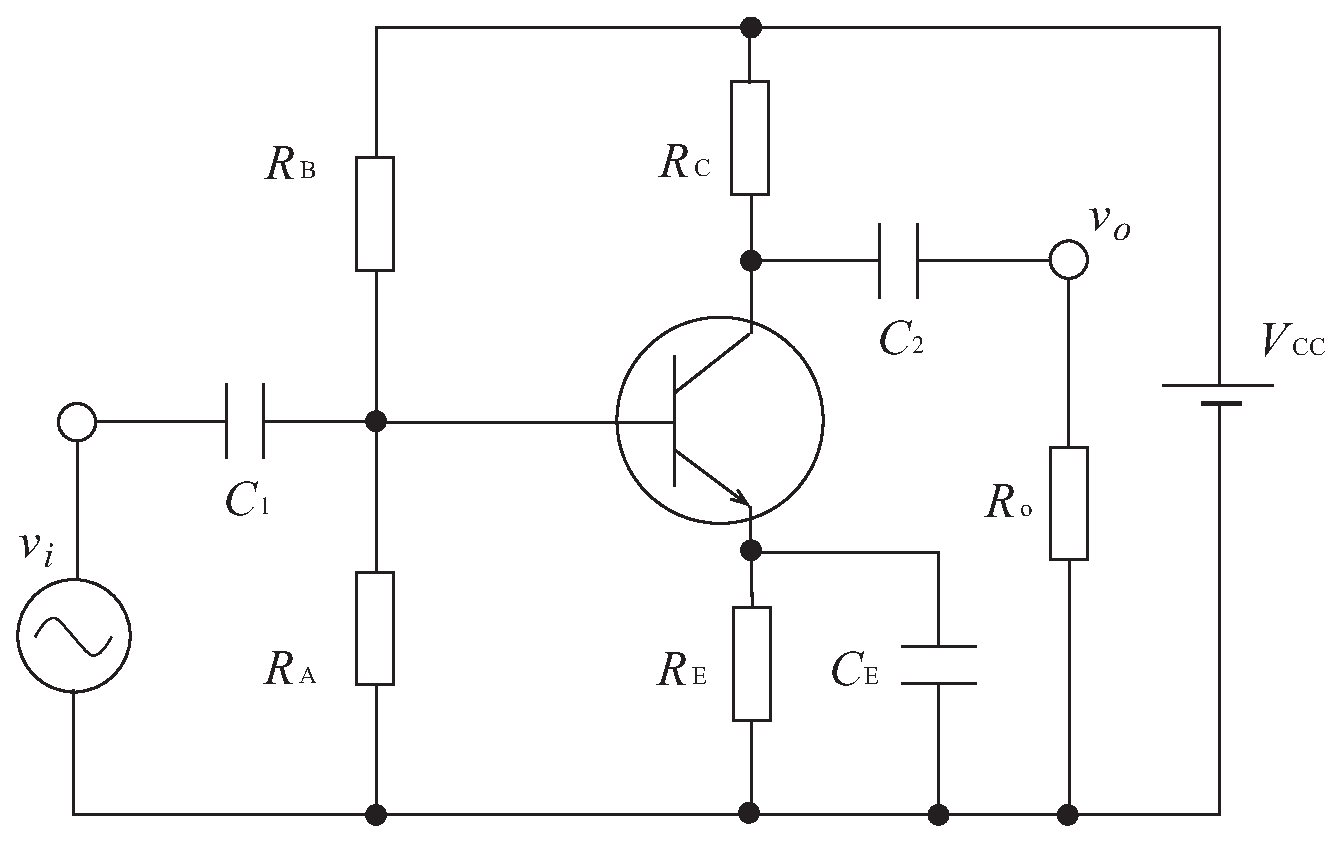
\includegraphics[keepaspectratio, scale=0.4, angle=0]
               {figs/eps/p87f1.eps}
               \caption{多段増幅回路の1段}
               \label{fig:p87f1}
\end{figure}


\subsection{バイアスと交流等価回路}

\subsection{電圧増幅度と周波数特性}

\end{comment}

\section{製作・実験 ①:静特性}

\subsection{出力特性:$V_{CE}\;-\;I_C$($I_B$一定):第1象限}

$V_{CE}-I_C$特性は出力特性とも呼ばれ、
ベース電流$I_B$一定の状態で、コレクタ-エミッタ間の電圧$V_{CE}$を変化させた時、
コレクタ電流$I_C$がどの様な変化をするかを示すもの\\

実験の手順は次の通り

\begin{enumerate}
\item[(1)] $V_{CE}=0.2$V にする(直流電源装置$E_C$を調節して)
\item[(2)] $I_B=20\;\mu$A にする(直流電源装置$E_B$、及び半固定抵抗器VRを調節して)
\item[(3)] $V_{CE}=0.2$Vを確認し、調整して、この時のコレクタ電流$I_C$を測定し、記録する
\item[(4)] $I_B=20\;\mu$A のまま、$V_{CE}$を$0.4$〜$10.0$V に変えて、その都度$I_C$を測定して記録する
\item[(5)] $V_{CE}=0.2$V に戻し、$I_B$を$40,\;60,\;80\;\mu$A と変えて、それぞれの場合に上の手順4を実施する    
\end{enumerate}

測定を終えたら、横軸にコレクタ-エミッタ間の電圧$V_{CE}$、縦軸にコレクタ電流$I_C$をとって、
第1象限のグラフを作図する

\vfill

\begin{figure}[H]
  \centering
   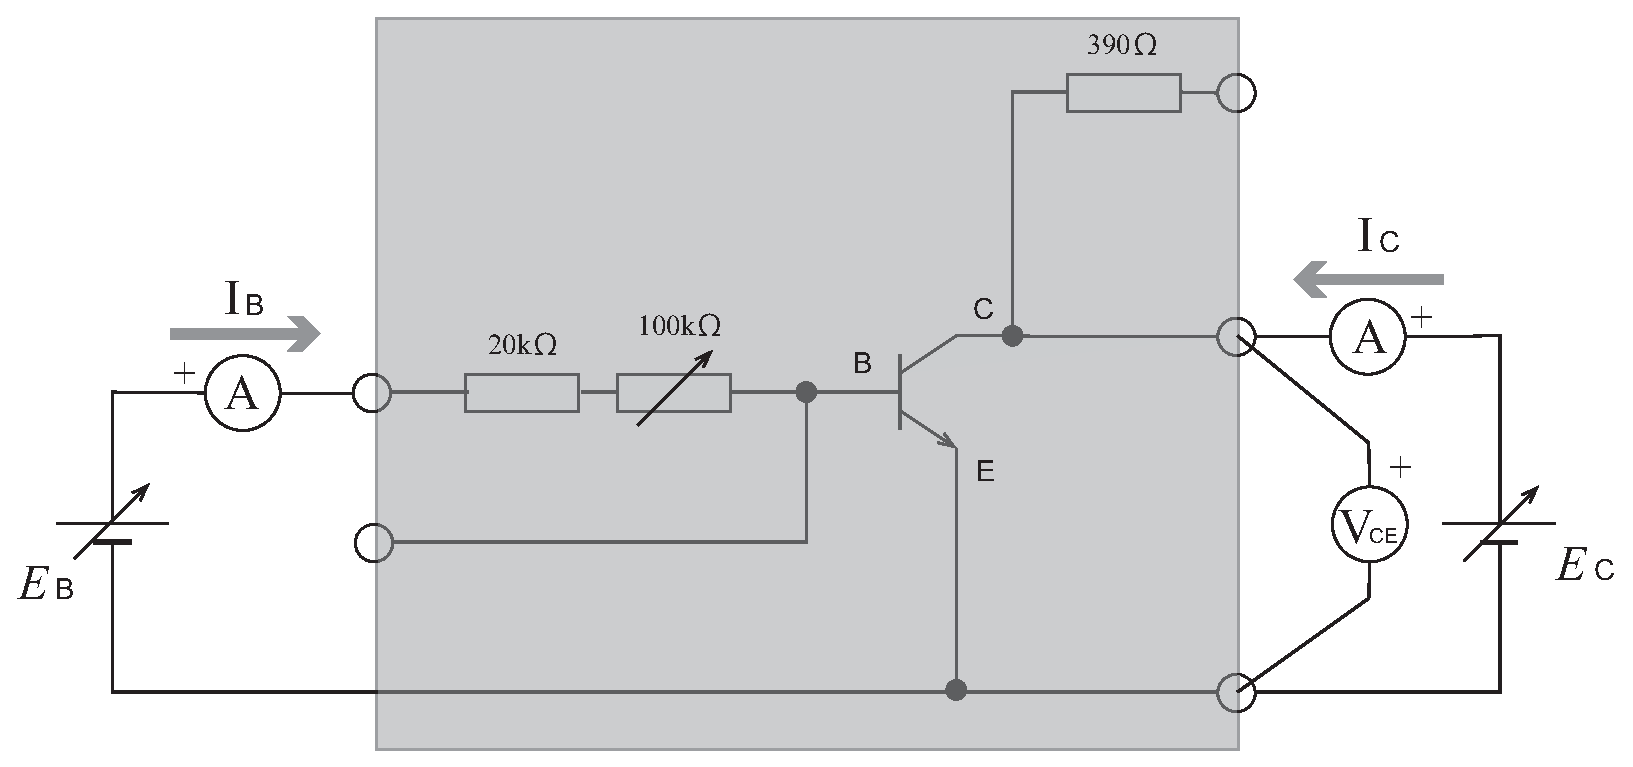
\includegraphics[keepaspectratio, scale=0.5, angle=0]
               {figs/eps/ex1.eps}
               \caption{出力特性$V_{CE}\;-\;I_C$($I_B$一定)}
               \label{fig:ex1}
\end{figure}

\vfill

\newpage

\subsubsection{2SC1815Orange}

\begingroup
\renewcommand{\arraystretch}{1.4}
\begin{table}[H]
  \begin{center}
  \caption{2SC1815O:$V_{CE}\;-\;I_C$特性:$I_B$一定}%\label{tbl:t1}\vspace{2mm}
  \begin{tabular}{|r|wr{2.5cm}|wr{2.5cm}|wr{2.5cm}|wr{2.5cm}|} \hline
    \rowcolor[rgb]{0.9, 0.9, 0.9}
    &\multicolumn{4}{c|}{\textbf{コレクタ電流 $I_C$[mA] (2SC1815O)}} \\ \hline
    \rowcolor[rgb]{0.9, 0.9, 0.9}
    \multicolumn{1}{|r|}{\textbf{$V_{CE}$[V]}} & \multicolumn{1}{c|}{\textbf{$I_B=20\mu$A}} & \multicolumn{1}{c|}{\textbf{$I_B=40\mu$A}} & \multicolumn{1}{c|}{\textbf{$I_B=60\mu$A}} & \multicolumn{1}{c|}{\textbf{$I_B=80\mu$A}} \\ \hline
    \multicolumn{1}{|r|}{\cellcolor[rgb]{0.9, 0.9, 0.9}\textbf{0.2}} & 2.251 & 4.282 & 6.240 & 7.971 \\ \hline
    \multicolumn{1}{|r|}{\cellcolor[rgb]{0.9, 0.9, 0.9}\textbf{0.4}} & 2.398 & 4.755 & 7.033 & 9.165 \\ \hline
    \multicolumn{1}{|r|}{\cellcolor[rgb]{0.9, 0.9, 0.9}\textbf{0.6}} & 2.402 & 4.771 & 7.108 & 9.424 \\ \hline
    \multicolumn{1}{|r|}{\cellcolor[rgb]{0.9, 0.9, 0.9}\textbf{0.8}} & 2.404 & 4.781 & 7.127 & 9.464 \\ \hline
    \multicolumn{1}{|r|}{\cellcolor[rgb]{0.9, 0.9, 0.9}\textbf{1.0}} & 2.408 & 4.791 & 7.143 & 9.495 \\ \hline
    \multicolumn{1}{|r|}{\cellcolor[rgb]{0.9, 0.9, 0.9}\textbf{2.0}} & 2.419 & 4.830 & 7.207 & 9.624 \\ \hline
    \multicolumn{1}{|r|}{\cellcolor[rgb]{0.9, 0.9, 0.9}\textbf{5.0}} & 2.448 & 4.924 & 7.397 & 9.943 \\ \hline
    \multicolumn{1}{|r|}{\cellcolor[rgb]{0.9, 0.9, 0.9}\textbf{8.0}} & 2.477 & 5.011 & 7.585 & 10.240 \\ \hline
    \multicolumn{1}{|r|}{\cellcolor[rgb]{0.9, 0.9, 0.9}\textbf{10.0}} & 2.495 & 5.057 & 7.700 & 10.430 \\ \hline
  \end{tabular}
  \end{center}
\end{table}
\endgroup

\subsubsection{2SC1815Yellow}

\begingroup
\renewcommand{\arraystretch}{1.4}
\begin{table}[H]
  \begin{center}
  \caption{2SC1815Y:$V_{CE}\;-\;I_C$特性:$I_B$一定}%\label{tbl:t1}\vspace{2mm}
  \begin{tabular}{|r|wr{2.5cm}|wr{2.5cm}|wr{2.5cm}|wr{2.5cm}|} \hline
    \rowcolor[rgb]{0.9, 0.9, 0.9}
    &\multicolumn{4}{c|}{\textbf{コレクタ電流 $I_C$[mA] (2SC1815Y)}} \\ \hline
    \rowcolor[rgb]{0.9, 0.9, 0.9}
    \multicolumn{1}{|r|}{\textbf{$V_{CE}$[V]}} & \multicolumn{1}{c|}{\textbf{$I_B=20\mu$A}} & \multicolumn{1}{c|}{\textbf{$I_B=40\mu$A}} & \multicolumn{1}{c|}{\textbf{$I_B=60\mu$A}} & \multicolumn{1}{c|}{\textbf{$I_B=80\mu$A}} \\ \hline
    \multicolumn{1}{|r|}{\cellcolor[rgb]{0.9, 0.9, 0.9}\textbf{0.2}} & 3.275 & 6.255 & 8.841 & 11.16 \\ \hline
    \multicolumn{1}{|r|}{\cellcolor[rgb]{0.9, 0.9, 0.9}\textbf{0.4}} & 3.526 & 6.961 & 10.20 & 12.98 \\ \hline
    \multicolumn{1}{|r|}{\cellcolor[rgb]{0.9, 0.9, 0.9}\textbf{0.6}} & 3.537 & 7.016 & 10.45 & 13.60 \\ \hline
    \multicolumn{1}{|r|}{\cellcolor[rgb]{0.9, 0.9, 0.9}\textbf{0.8}} & 3.545 & 7.047 & 10.52 & 13.79 \\ \hline
    \multicolumn{1}{|r|}{\cellcolor[rgb]{0.9, 0.9, 0.9}\textbf{1.0}} & 3.553 & 7.068 & 10.63 & 13.90 \\ \hline
    \multicolumn{1}{|r|}{\cellcolor[rgb]{0.9, 0.9, 0.9}\textbf{2.0}} & 3.600 & 7.189 & 10.88 & 14.32 \\ \hline
    \multicolumn{1}{|r|}{\cellcolor[rgb]{0.9, 0.9, 0.9}\textbf{5.0}} & 3.698 & 7.550 & 11.65 & 15.54 \\ \hline
    \multicolumn{1}{|r|}{\cellcolor[rgb]{0.9, 0.9, 0.9}\textbf{8.0}} & 3.811 & 7.900 & 12.42 & 16.88 \\ \hline
    \multicolumn{1}{|r|}{\cellcolor[rgb]{0.9, 0.9, 0.9}\textbf{10.0}} & 3.879 & 8.148 & 13.06 & 17.79 \\ \hline
  \end{tabular}
  \end{center}
\end{table}
\endgroup

\subsubsection{2SC1815GReen}

\begingroup
\renewcommand{\arraystretch}{1.4}
\begin{table}[H]
  \begin{center}
  \caption{2SC1815GR:$V_{CE}\;-\;I_C$特性:$I_B$一定}%\label{tbl:t1}\vspace{2mm}
  \begin{tabular}{|r|wr{2.5cm}|wr{2.5cm}|wr{2.5cm}|wr{2.5cm}|} \hline
    \rowcolor[rgb]{0.9, 0.9, 0.9}
    &\multicolumn{4}{c|}{\textbf{コレクタ電流 $I_C$[mA] (2SC1815GR)}} \\ \hline
    \rowcolor[rgb]{0.9, 0.9, 0.9}
    \multicolumn{1}{|r|}{\textbf{$V_{CE}$[V]}} & \multicolumn{1}{c|}{\textbf{$I_B=20\mu$A}} & \multicolumn{1}{c|}{\textbf{$I_B=40\mu$A}} & \multicolumn{1}{c|}{\textbf{$I_B=60\mu$A}} & \multicolumn{1}{c|}{\textbf{$I_B=80\mu$A}} \\ \hline
    \multicolumn{1}{|r|}{\cellcolor[rgb]{0.9, 0.9, 0.9}\textbf{0.2}} & 5.218 & 9.108 & 12.26 & 14.98 \\ \hline
    \multicolumn{1}{|r|}{\cellcolor[rgb]{0.9, 0.9, 0.9}\textbf{0.4}} & 5.860 & 11.068 & 15.03 & 18.18 \\ \hline
    \multicolumn{1}{|r|}{\cellcolor[rgb]{0.9, 0.9, 0.9}\textbf{0.6}} & 5.898 & 11.62 & 16.60 & 20.40 \\ \hline
    \multicolumn{1}{|r|}{\cellcolor[rgb]{0.9, 0.9, 0.9}\textbf{0.8}} & 5.922 & 11.70 & 17.24 & 22.02 \\ \hline
    \multicolumn{1}{|r|}{\cellcolor[rgb]{0.9, 0.9, 0.9}\textbf{1.0}} & 5.948 & 11.76 & 17.42 & 22.90 \\ \hline
    \multicolumn{1}{|r|}{\cellcolor[rgb]{0.9, 0.9, 0.9}\textbf{2.0}} & 6.033 & 11.99 & 17.89 & 24.18 \\ \hline
    \multicolumn{1}{|r|}{\cellcolor[rgb]{0.9, 0.9, 0.9}\textbf{5.0}} & 6.302 & 12.75 & 19.36 & 27.11 \\ \hline
    \multicolumn{1}{|r|}{\cellcolor[rgb]{0.9, 0.9, 0.9}\textbf{8.0}} & 6.495 & 13.52 & 20.96 & 30.47 \\ \hline
    \multicolumn{1}{|r|}{\cellcolor[rgb]{0.9, 0.9, 0.9}\textbf{10.0}} & 6.691 & 14.12 & 22.34 & 32.60 \\ \hline
  \end{tabular}
  \end{center}
\end{table}
\endgroup

\subsubsection{2SC1815BLue}

\begingroup
\renewcommand{\arraystretch}{1.4}
\begin{table}[H]
  \begin{center}
  \caption{2SC1815BL:$V_{CE}\;-\;I_C$特性:$I_B$一定}%\label{tbl:t1}\vspace{2mm}
  \begin{tabular}{|r|wr{2.5cm}|wr{2.5cm}|wr{2.5cm}|wr{2.5cm}|} \hline
    \rowcolor[rgb]{0.9, 0.9, 0.9}
    &\multicolumn{4}{c|}{\textbf{コレクタ電流 $I_C$[mA] (2SC1815BL)}} \\ \hline
    \rowcolor[rgb]{0.9, 0.9, 0.9}
    \multicolumn{1}{|r|}{\textbf{$V_{CE}$[V]}} & \multicolumn{1}{c|}{\textbf{$I_B=20\mu$A}} & \multicolumn{1}{c|}{\textbf{$I_B=40\mu$A}} & \multicolumn{1}{c|}{\textbf{$I_B=60\mu$A}} & \multicolumn{1}{c|}{\textbf{$I_B=80\mu$A}} \\ \hline
    \multicolumn{1}{|r|}{\cellcolor[rgb]{0.9, 0.9, 0.9}\textbf{0.2}} & 8.919 & 14.56 & 18.70 & 22.45 \\ \hline
    \multicolumn{1}{|r|}{\cellcolor[rgb]{0.9, 0.9, 0.9}\textbf{0.4}} & 10.684 & 17.98 & 23.04 & 27.13 \\ \hline
    \multicolumn{1}{|r|}{\cellcolor[rgb]{0.9, 0.9, 0.9}\textbf{0.6}} & 10.998 & 19.90 & 25.69 & 30.22 \\ \hline
    \multicolumn{1}{|r|}{\cellcolor[rgb]{0.9, 0.9, 0.9}\textbf{0.8}} & 11.124 & 21.02 & 27.90 & 32.77 \\ \hline
    \multicolumn{1}{|r|}{\cellcolor[rgb]{0.9, 0.9, 0.9}\textbf{1.0}} & 11.19 & 21.66 & 29.44 & 35.13 \\ \hline
    \multicolumn{1}{|r|}{\cellcolor[rgb]{0.9, 0.9, 0.9}\textbf{2.0}} & 11.51 & 22.71 & 32.23 & 41.80 \\ \hline
    \multicolumn{1}{|r|}{\cellcolor[rgb]{0.9, 0.9, 0.9}\textbf{5.0}} & 12.46 & 25.51 & 37.41 & 49.16 \\ \hline
    \multicolumn{1}{|r|}{\cellcolor[rgb]{0.9, 0.9, 0.9}\textbf{8.0}} & 13.41 & 28.32 & 41.66 & 53.90 \\ \hline
    \multicolumn{1}{|r|}{\cellcolor[rgb]{0.9, 0.9, 0.9}\textbf{10.0}} & 14.14 & 29.68 & 43.92 & 56.02 \\ \hline
  \end{tabular}
  \end{center}
\end{table}
\endgroup

\newpage

\begin{figure}[H]
  \centering
   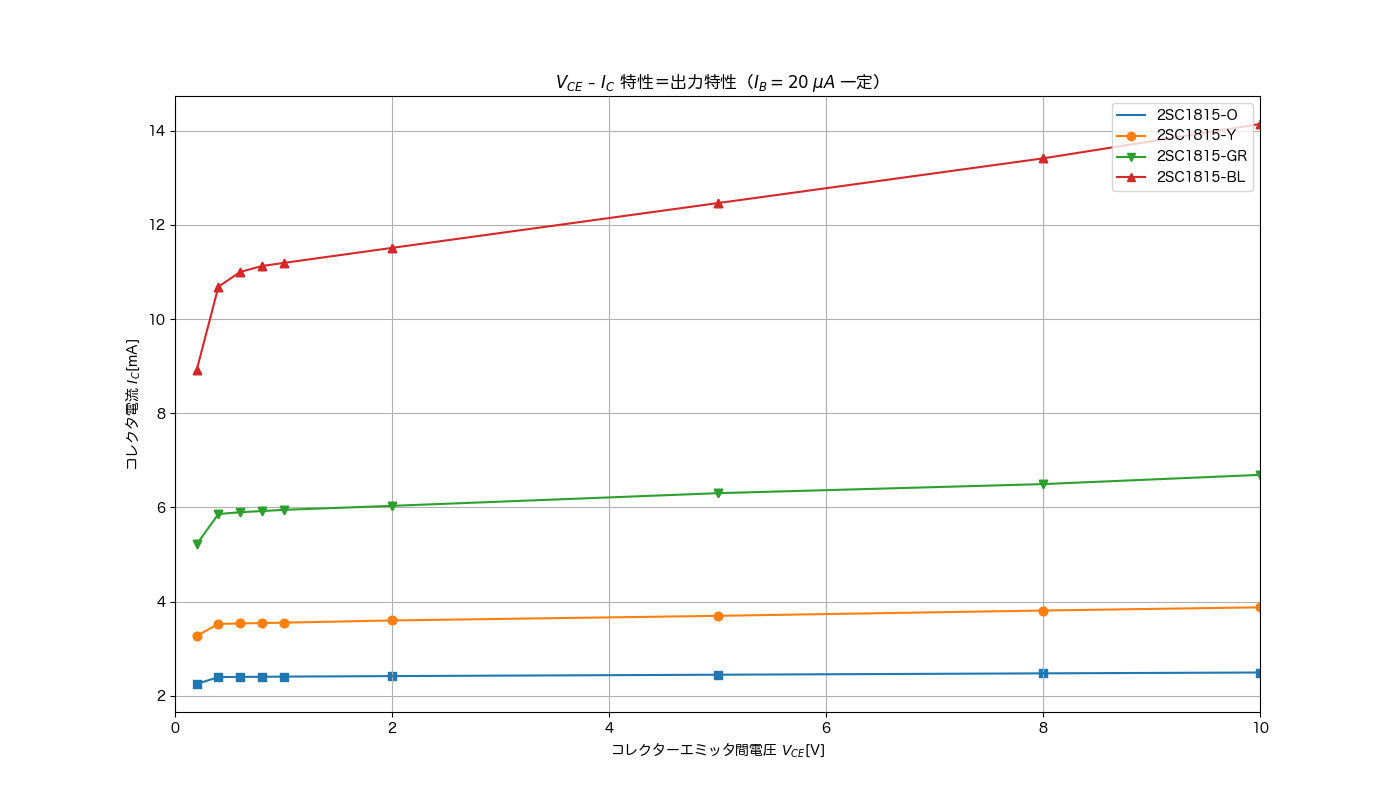
\includegraphics[keepaspectratio, scale=0.48, angle=0]
               {figs/png/staticE01Ib20.png}
               \caption{$I_B=20\;\mu$A}
               \label{fig:ex011}
\end{figure}

\begin{figure}[H]
  \centering
   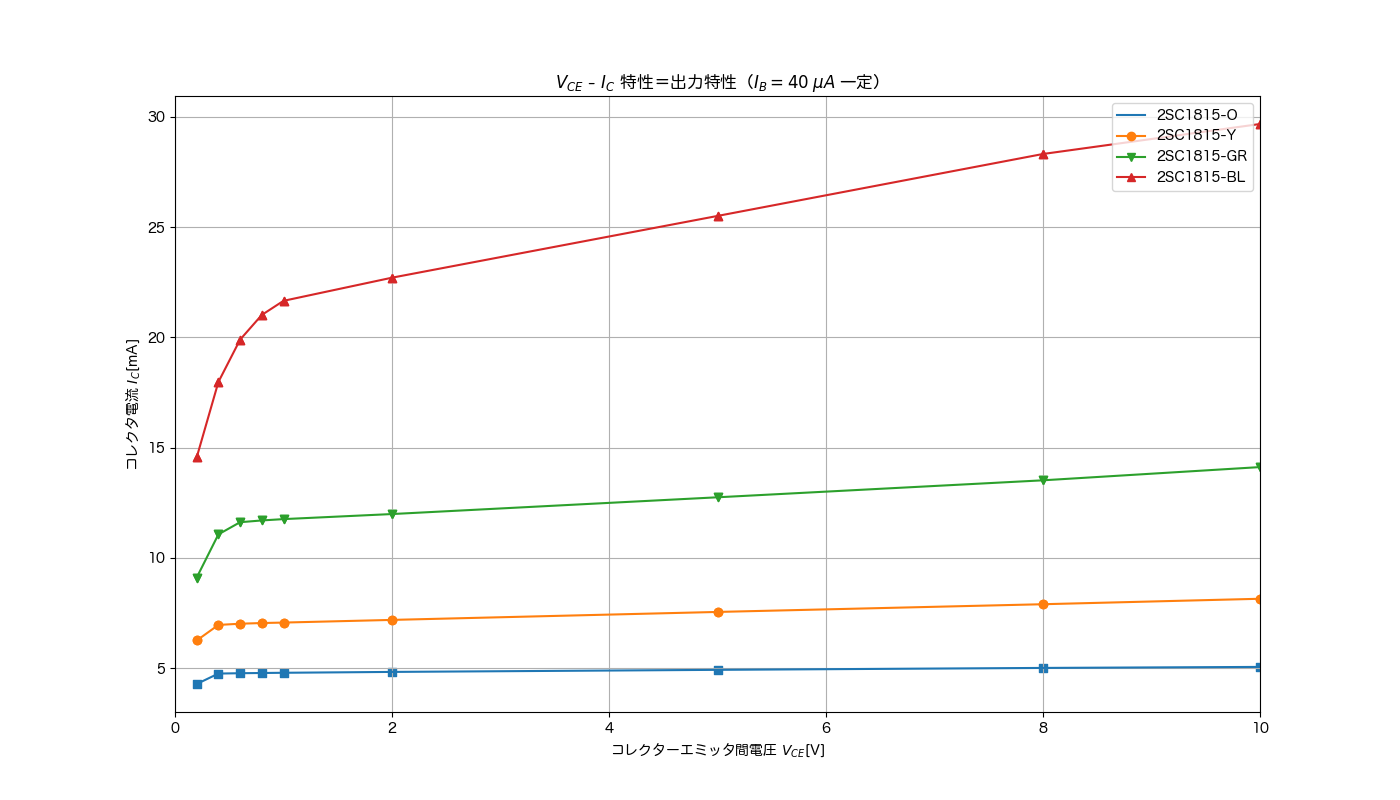
\includegraphics[keepaspectratio, scale=0.48, angle=0]
             {figs/png/staticE01Ib40.png}
             \caption{$I_B=40\;\mu$A}
             \label{fig:ex012}
\end{figure}

\newpage

\begin{figure}[H]
  \centering
   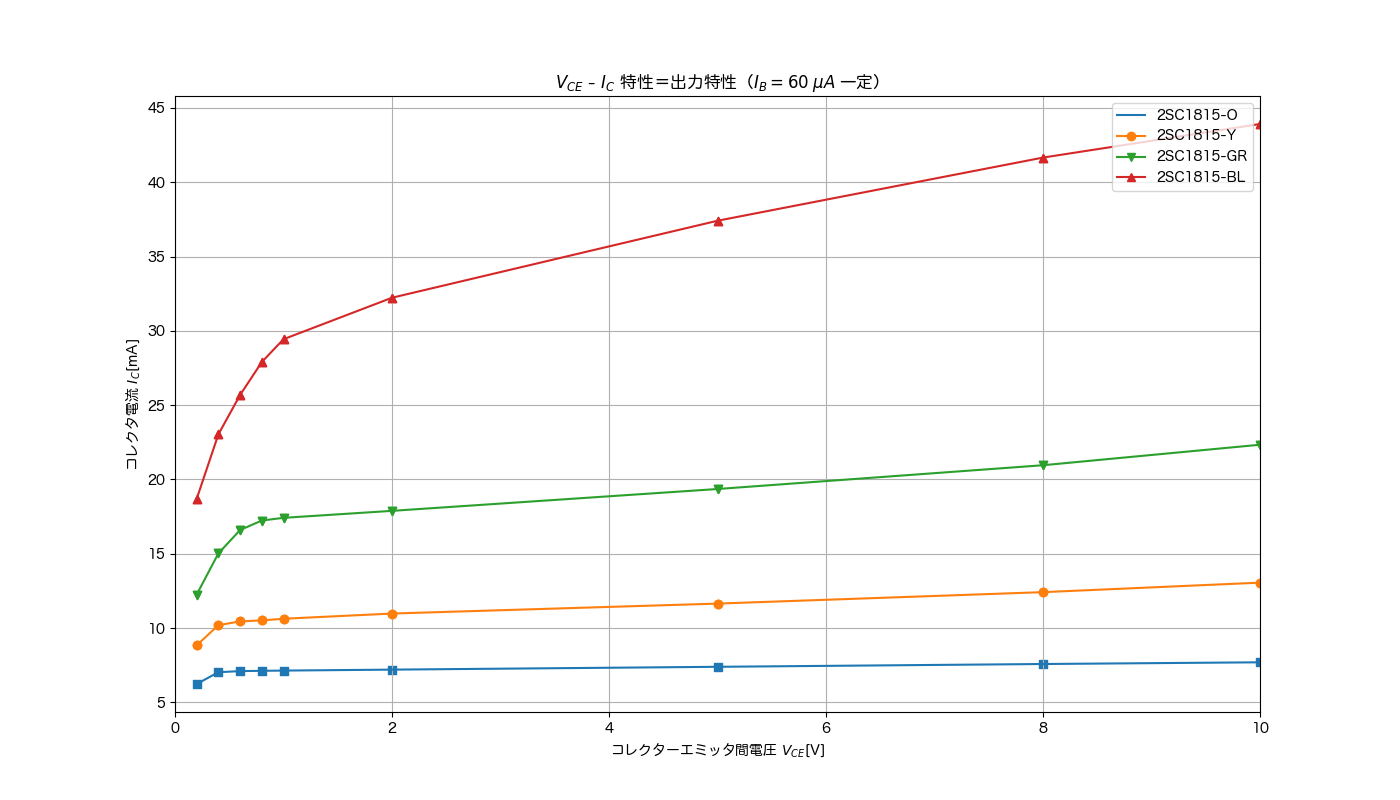
\includegraphics[keepaspectratio, scale=0.48, angle=0]
               {figs/png/staticE01Ib60.png}
               \caption{$I_B=60\;\mu$A}
               \label{fig:ex013}
\end{figure}

\begin{figure}[H]
  \centering
   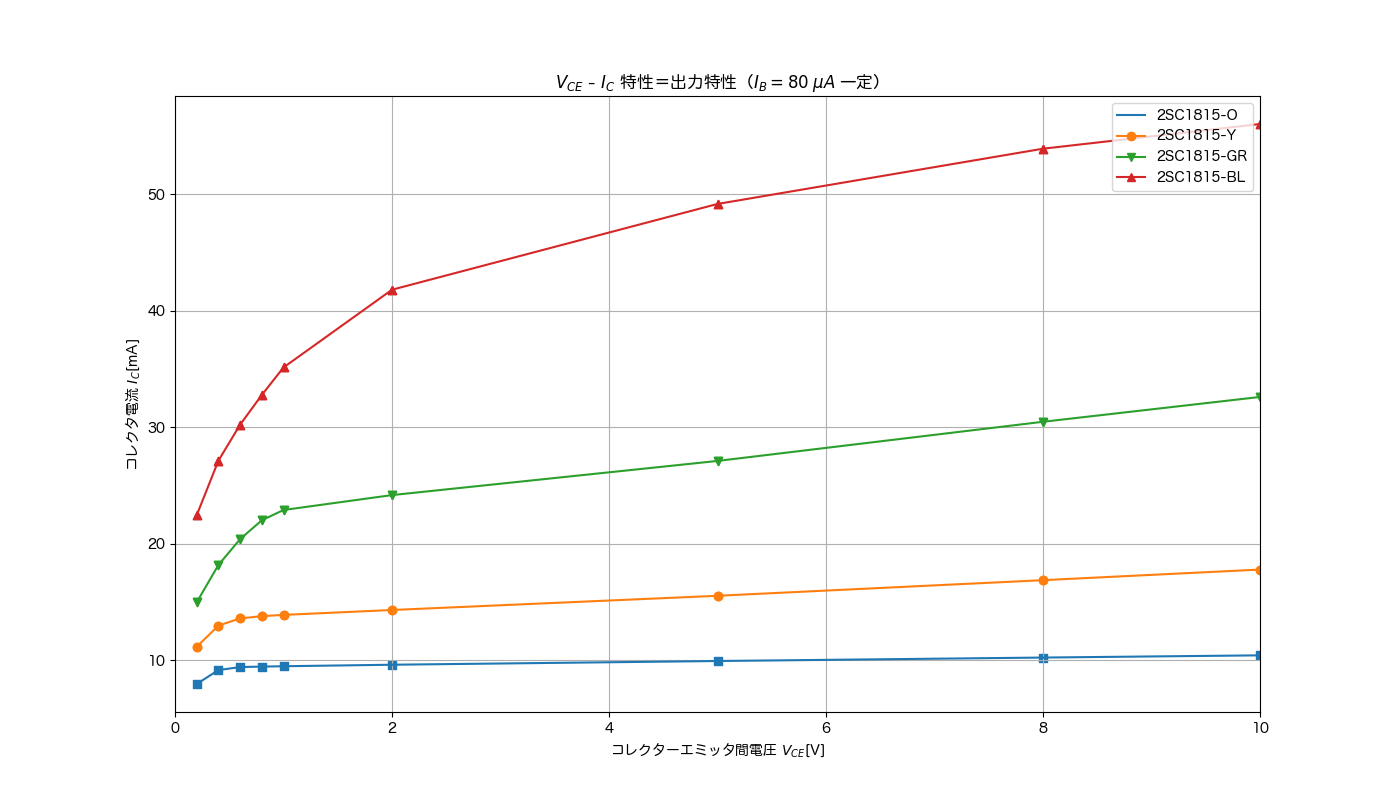
\includegraphics[keepaspectratio, scale=0.48, angle=0]
             {figs/png/staticE01Ib80.png}
             \caption{$I_B=80\;\mu$A}
             \label{fig:ex014}
\end{figure}

\newpage

\subsection{$I_B\;-\;I_C$特性($V_{CE}=5V$一定):第2象限}

$I_B\;-\;I_C$特性は、コレクタ-エミッタ間の電圧$V_{CE}$を一定にした状態で、
ベース電流$I_B$を変化させた時に、コレクタ電流$I_C$がどの様に変化するかを示すもの

この特性の傾き$I_C/I_B$は、直流電流増幅率$h_{FE}$と呼ばれる\\

実験の手順は次の通り

\begin{enumerate}
\item[(1)] $V_{CE}=5$V となるように$E_C$を調整し、測定中はこの値を維持する
\item[(2)] $E_B$(と必要に応じて可変抵抗器)を調整して、ベース電流$I_B$を$0$〜$80\;\mu$A まで$10\;\mu$A ずつ変化させ、
その都度コレクタ電流$I_C$を測定して記録する 
\end{enumerate}

測定を終えたら、横軸にベース電流$I_B$、縦軸にコレクタ電流$I_C$をとって、第2象限のグラフを作図し、
直流電流増幅率を求める

\vfill

\begin{figure}[H]
  \centering
   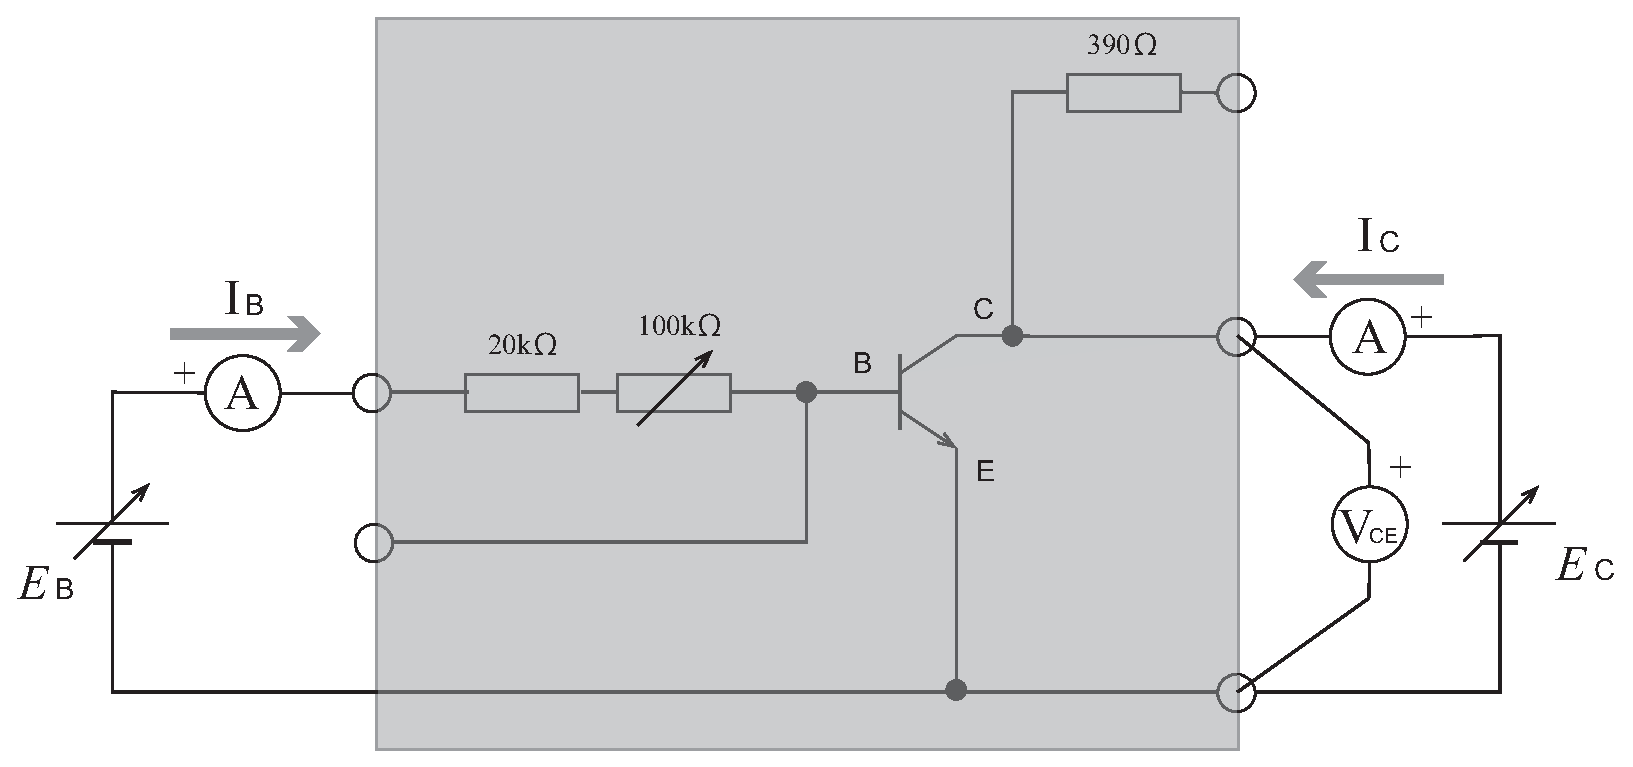
\includegraphics[keepaspectratio, scale=0.5, angle=0]
               {figs/eps/ex1.eps}
               \caption{$I_B\;-\;I_C$特性($V_{CE}=5$V 一定)}
               \label{fig:ex2}
\end{figure}

\vfill

\newpage

\subsubsection{2SC1815Orange}

\begingroup
\renewcommand{\arraystretch}{1.6}
\begin{table}[H]
  \begin{center}
  \caption{2SC1815O:$I_{B}\;-\;I_C$特性:$V_{CE}=5$V一定}%\label{tbl:t5}\vspace{2mm}
  \begin{tabular}{|r|wr{1cm}|wr{1cm}|wr{1cm}|wr{1cm}|wr{1cm}|wr{1cm}|wr{1cm}|wr{1cm}|wr{1cm}|} \hline
    \rowcolor[rgb]{0.9, 0.9, 0.9}
    \multicolumn{1}{|r|}{\textbf{$I_B$[$\mu$A]}} & \multicolumn{1}{c|}{\textbf{0}} & \multicolumn{1}{c|}{\textbf{10}} & \multicolumn{1}{c|}{\textbf{20}} & \multicolumn{1}{c|}{\textbf{30}} & \multicolumn{1}{c|}{\textbf{40}} & \multicolumn{1}{c|}{\textbf{50}} & \multicolumn{1}{c|}{\textbf{60}} & \multicolumn{1}{c|}{\textbf{70}} & \multicolumn{1}{c|}{\textbf{80}}\\ \hline
    \multicolumn{1}{|r|}{\cellcolor[rgb]{0.9, 0.9, 0.9}\textbf{$I_C$[mA]}} & 0 & 1.229 & 2.457 & 3.691 & 4.924 & 6.179 & 7.427 & 8.689 & 9.958 \\ \hline
  \end{tabular}
  \end{center}
\end{table}
\endgroup

\vfill

\subsubsection{2SC1815Yellow}

\begingroup
\renewcommand{\arraystretch}{1.6}
\begin{table}[H]
  \begin{center}
  \caption{2SC1815Y:$I_{B}\;-\;I_C$特性:$V_{CE}=5$V一定}%\label{tbl:t5}\vspace{2mm}
  \begin{tabular}{|r|wr{1cm}|wr{1cm}|wr{1cm}|wr{1cm}|wr{1cm}|wr{1cm}|wr{1cm}|wr{1cm}|wr{1cm}|} \hline
    \rowcolor[rgb]{0.9, 0.9, 0.9}
    \multicolumn{1}{|r|}{\textbf{$I_B$[$\mu$A]}} & \multicolumn{1}{c|}{\textbf{0}} & \multicolumn{1}{c|}{\textbf{10}} & \multicolumn{1}{c|}{\textbf{20}} & \multicolumn{1}{c|}{\textbf{30}} & \multicolumn{1}{c|}{\textbf{40}} & \multicolumn{1}{c|}{\textbf{50}} & \multicolumn{1}{c|}{\textbf{60}} & \multicolumn{1}{c|}{\textbf{70}} & \multicolumn{1}{c|}{\textbf{80}}\\ \hline
    \multicolumn{1}{|r|}{\cellcolor[rgb]{0.9, 0.9, 0.9}\textbf{$I_C$[mA]}} & 0 & 1.814 & 3.679 & 5.565 & 7.505 & 9.453 & 11.44 & 13.49 & 15.50 \\ \hline
  \end{tabular}
  \end{center}
\end{table}
\endgroup

\vfill

\subsubsection{2SC1815GReen}

\begingroup
\renewcommand{\arraystretch}{1.6}
\begin{table}[H]
  \begin{center}
  \caption{2SC1815GR:$I_{B}\;-\;I_C$特性:$V_{CE}=5$V一定}%\label{tbl:t5}\vspace{2mm}
  \begin{tabular}{|r|wr{1cm}|wr{1cm}|wr{1cm}|wr{1cm}|wr{1cm}|wr{1cm}|wr{1cm}|wr{1cm}|wr{1cm}|} \hline
    \rowcolor[rgb]{0.9, 0.9, 0.9}
    \multicolumn{1}{|r|}{\textbf{$I_B$[$\mu$A]}} & \multicolumn{1}{c|}{\textbf{0}} & \multicolumn{1}{c|}{\textbf{10}} & \multicolumn{1}{c|}{\textbf{20}} & \multicolumn{1}{c|}{\textbf{30}} & \multicolumn{1}{c|}{\textbf{40}} & \multicolumn{1}{c|}{\textbf{50}} & \multicolumn{1}{c|}{\textbf{60}} & \multicolumn{1}{c|}{\textbf{70}} & \multicolumn{1}{c|}{\textbf{80}}\\ \hline
    \multicolumn{1}{|r|}{\cellcolor[rgb]{0.9, 0.9, 0.9}\textbf{$I_C$[mA]}} & 0 & 3.098 & 6.306 & 9.530 & 12.84 & 16.20 & 19.63 & 23.10 & 26.62 \\ \hline
  \end{tabular}
  \end{center}
\end{table}
\endgroup

\vfill

\subsubsection{2SC1815BLue}

\begingroup
\renewcommand{\arraystretch}{1.6}
\begin{table}[H]
  \begin{center}
  \caption{2SC1815BL:$I_{B}\;-\;I_C$特性:$V_{CE}=5$V一定}%\label{tbl:t5}\vspace{2mm}
  \begin{tabular}{|r|wr{1cm}|wr{1cm}|wr{1cm}|wr{1cm}|wr{1cm}|wr{1cm}|wr{1cm}|wr{1cm}|wr{1cm}|} \hline
    \rowcolor[rgb]{0.9, 0.9, 0.9}
    \multicolumn{1}{|r|}{\textbf{$I_B$[$\mu$A]}} & \multicolumn{1}{c|}{\textbf{0}} & \multicolumn{1}{c|}{\textbf{10}} & \multicolumn{1}{c|}{\textbf{20}} & \multicolumn{1}{c|}{\textbf{30}} & \multicolumn{1}{c|}{\textbf{40}} & \multicolumn{1}{c|}{\textbf{50}} & \multicolumn{1}{c|}{\textbf{60}} & \multicolumn{1}{c|}{\textbf{70}} & \multicolumn{1}{c|}{\textbf{80}}\\ \hline
    \multicolumn{1}{|r|}{\cellcolor[rgb]{0.9, 0.9, 0.9}\textbf{$I_C$[mA]}} & 0 & 6.189 & 12.43 & 18.64 & 24.92 & 31.09 & 37.26 & 42.95 & 48.31\\ \hline
  \end{tabular}
  \end{center}
\end{table}
\endgroup

\newpage

\begin{figure}[H]
  \centering
   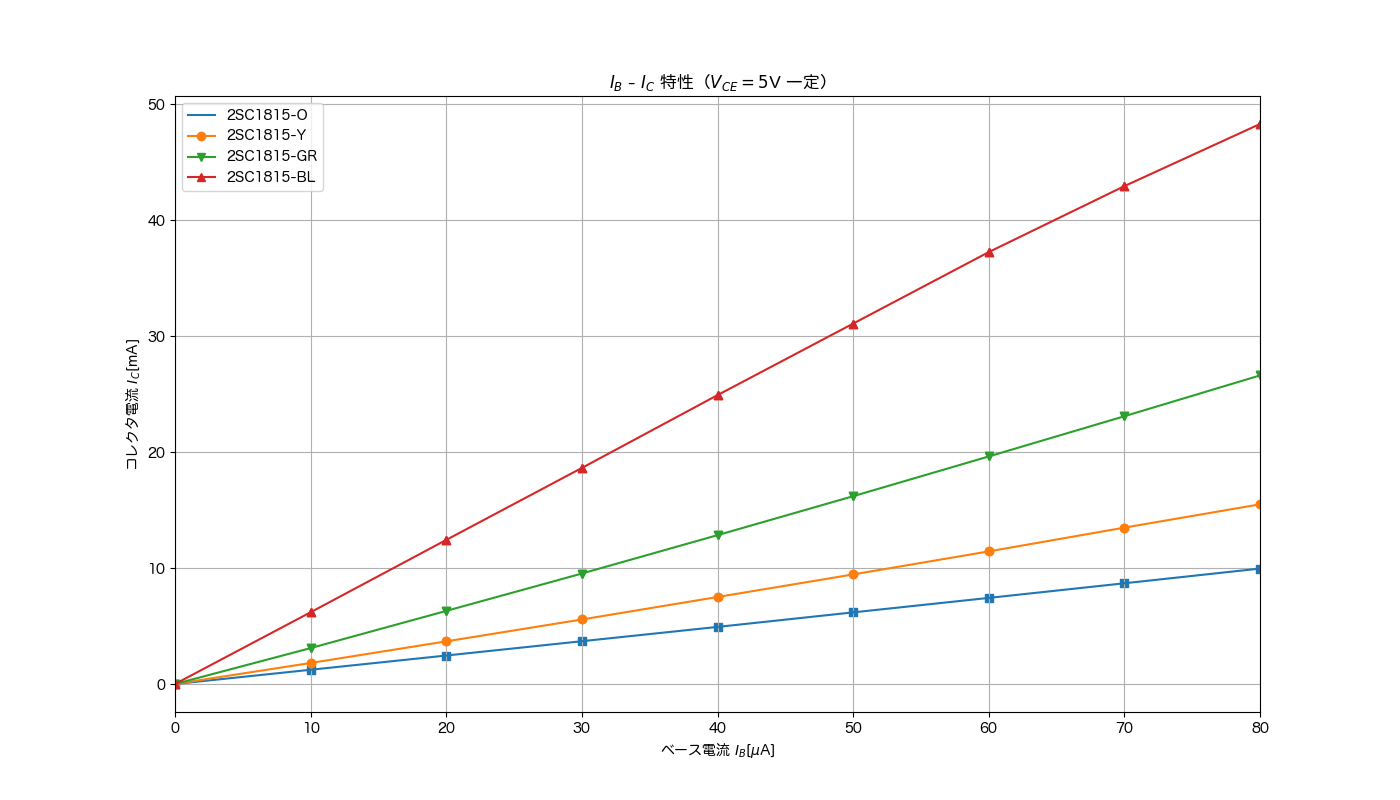
\includegraphics[keepaspectratio, scale=0.48, angle=0]
               {figs/png/staticE02.png}
               \caption{$I_{B}\;-\;I_C\;$特性}
               \label{fig:ex02}
\end{figure}

\newpage

\subsection{入力特性$V_{BE}\;-\;I_B$($V_{CE}=5V$一定):第3象限}

$V_{BE}\;-\;I_B$特性は入力特性とも呼ばれ、コレクタ-エミッタ間の電圧$V_{CE}$を一定にした状態で、
ベース-エミッタ間の電圧$V_{BE}$を変化させた時、ベース電流$I_B$がどの様に変わるかを示すもの

この特性は、ダイオードの順方向特性とほぼ同じになる\\

実験の手順は次の通り

\begin{enumerate}
\item[(1)] $V_{CC}=5$V となる様に$E_C$を調整し、測定中はこの値を維持する
\item[(2)] $E_B$(必要に応じて可変抵抗器)を調整して、ベース-エミッタ間の電圧$V_{BE}$を変化させ、その都度ベース電流$I_B$を測定し記録する
\end{enumerate}

測定を終えたら、横軸にベース電流を、縦軸にベースエミッタ間の電圧をとって、
第3象限のグラフを作図する

\vfill

\begin{figure}[H]
  \centering
   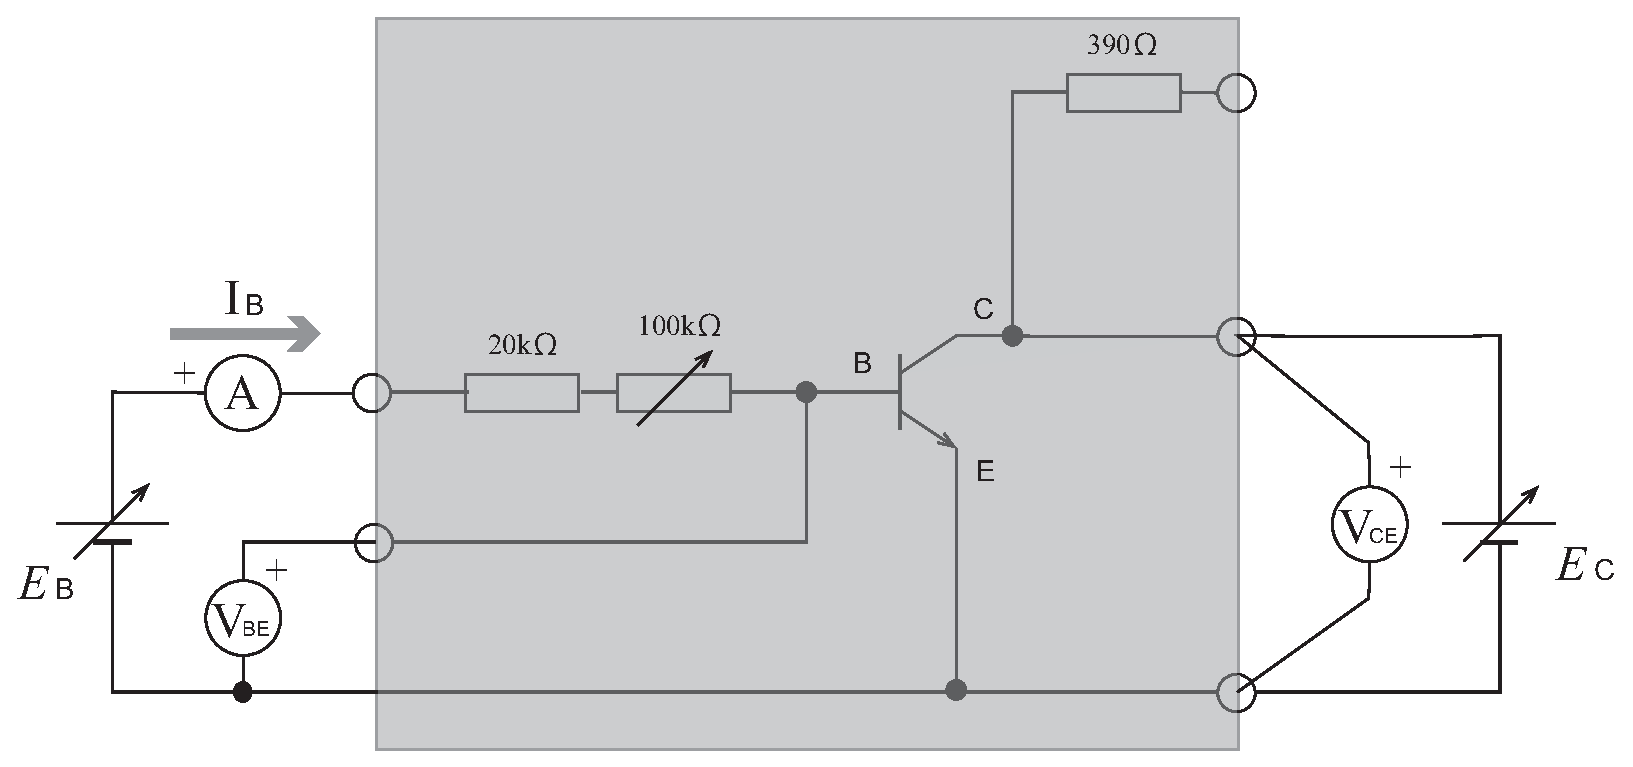
\includegraphics[keepaspectratio, scale=0.5, angle=0]
               {figs/eps/ex3.eps}
               \caption{入力特性$V_{BE}\;-\;I_B$($V_{CE}=5$V 一定)}
               \label{fig:ex3}
\end{figure}

\vfill

\newpage

\subsubsection{2SC1815Orange}

\begingroup
\renewcommand{\arraystretch}{1.6}
\begin{table}[H]
  \begin{center}
  \caption{2SC1815O:$V_{BE}\;-\;I_B$特性:$V_{CE}=5$V一定}%\label{tbl:t9}\vspace{2mm}
  \begin{tabular}{|r|wr{1cm}|wr{1cm}|wr{1cm}|wr{1cm}|wr{1cm}|wr{1cm}|wr{1cm}|wr{1cm}|wr{1cm}|} \hline
    \multicolumn{1}{|r|}{\cellcolor[rgb]{0.9, 0.9, 0.9}\textbf{$V_{BE}$[V]}} & \multicolumn{1}{c|}{\cellcolor[rgb]{0.9, 0.9, 0.9}\textbf{0.2}} & \multicolumn{1}{c|}{\cellcolor[rgb]{0.9, 0.9, 0.9}\textbf{0.3}} & \multicolumn{1}{c|}{\cellcolor[rgb]{0.9, 0.9, 0.9}\textbf{0.4}} & \multicolumn{1}{c|}{\cellcolor[rgb]{0.9, 0.9, 0.9}\textbf{0.5}} & \multicolumn{1}{c|}{\cellcolor[rgb]{0.9, 0.9, 0.9}\textbf{0.6}} & 0.664 & 0.6814 & 0.7036 & 0.7136 \\ \hline
    \multicolumn{1}{|r|}{\cellcolor[rgb]{0.9, 0.9, 0.9}\textbf{$I_B$[$\mu$A]}} & 0.01 & 0.02 & 0.03 & 0.10 & 1.21 & \multicolumn{1}{c|}{\cellcolor[rgb]{0.9, 0.9, 0.9}\textbf{10.0}} & \multicolumn{1}{c|}{\cellcolor[rgb]{0.9, 0.9, 0.9}\textbf{20.0}} & \multicolumn{1}{c|}{\cellcolor[rgb]{0.9, 0.9, 0.9}\textbf{50.0}} & \multicolumn{1}{c|}{\cellcolor[rgb]{0.9, 0.9, 0.9}\textbf{80.0}}\\ \hline
  \end{tabular}
  \end{center}
\end{table}
\endgroup

\vfill

\subsubsection{2SC1815Yellow}

\begingroup
\renewcommand{\arraystretch}{1.6}
\begin{table}[H]
  \begin{center}
  \caption{2SC1815Y:$V_{BE}\;-\;I_B$特性:$V_{CE}=5$V一定}%\label{tbl:t9}\vspace{2mm}
  \begin{tabular}{|r|wr{1cm}|wr{1cm}|wr{1cm}|wr{1cm}|wr{1cm}|wr{1cm}|wr{1cm}|wr{1cm}|wr{1cm}|} \hline
    \multicolumn{1}{|r|}{\cellcolor[rgb]{0.9, 0.9, 0.9}\textbf{$V_{BE}$[V]}} & \multicolumn{1}{c|}{\cellcolor[rgb]{0.9, 0.9, 0.9}\textbf{0.2}} & \multicolumn{1}{c|}{\cellcolor[rgb]{0.9, 0.9, 0.9}\textbf{0.3}} & \multicolumn{1}{c|}{\cellcolor[rgb]{0.9, 0.9, 0.9}\textbf{0.4}} & \multicolumn{1}{c|}{\cellcolor[rgb]{0.9, 0.9, 0.9}\textbf{0.5}} & \multicolumn{1}{c|}{\cellcolor[rgb]{0.9, 0.9, 0.9}\textbf{0.6}} & 0.6523 & 0.6670 & 0.6787 & 0.6838 \\ \hline
    \multicolumn{1}{|r|}{\cellcolor[rgb]{0.9, 0.9, 0.9}\textbf{$I_B$[$\mu$A]}} & 0.01 & 0.02 & 0.03 & 0.12 & 1.48 & \multicolumn{1}{c|}{\cellcolor[rgb]{0.9, 0.9, 0.9}\textbf{10.0}} & \multicolumn{1}{c|}{\cellcolor[rgb]{0.9, 0.9, 0.9}\textbf{20.0}} & \multicolumn{1}{c|}{\cellcolor[rgb]{0.9, 0.9, 0.9}\textbf{50.0}} & \multicolumn{1}{c|}{\cellcolor[rgb]{0.9, 0.9, 0.9}\textbf{80.0}}\\ \hline
  \end{tabular}
  \end{center}
\end{table}
\endgroup

\vfill

\subsubsection{2SC1815GReen}

\begingroup
\renewcommand{\arraystretch}{1.6}
\begin{table}[H]
  \begin{center}
  \caption{2SC1815GR:$V_{BE}\;-\;I_B$特性:$V_{CE}=5$V一定}%\label{tbl:t9}\vspace{2mm}
  \begin{tabular}{|r|wr{1cm}|wr{1cm}|wr{1cm}|wr{1cm}|wr{1cm}|wr{1cm}|wr{1cm}|wr{1cm}|wr{1cm}|} \hline
    \multicolumn{1}{|r|}{\cellcolor[rgb]{0.9, 0.9, 0.9}\textbf{$V_{BE}$[V]}} & \multicolumn{1}{c|}{\cellcolor[rgb]{0.9, 0.9, 0.9}\textbf{0.2}} & \multicolumn{1}{c|}{\cellcolor[rgb]{0.9, 0.9, 0.9}\textbf{0.3}} & \multicolumn{1}{c|}{\cellcolor[rgb]{0.9, 0.9, 0.9}\textbf{0.4}} & \multicolumn{1}{c|}{\cellcolor[rgb]{0.9, 0.9, 0.9}\textbf{0.5}} & \multicolumn{1}{c|}{\cellcolor[rgb]{0.9, 0.9, 0.9}\textbf{0.6}} & 0.661 & 0.677 & 0.697 & 0.705 \\ \hline
    \multicolumn{1}{|r|}{\cellcolor[rgb]{0.9, 0.9, 0.9}\textbf{$I_B$[$\mu$A]}} & 0 & 0 & 0.01 & 0.07 & 1.24 & \multicolumn{1}{c|}{\cellcolor[rgb]{0.9, 0.9, 0.9}\textbf{10.0}} & \multicolumn{1}{c|}{\cellcolor[rgb]{0.9, 0.9, 0.9}\textbf{20.0}} & \multicolumn{1}{c|}{\cellcolor[rgb]{0.9, 0.9, 0.9}\textbf{50.0}} & \multicolumn{1}{c|}{\cellcolor[rgb]{0.9, 0.9, 0.9}\textbf{80.0}}\\ \hline
  \end{tabular}
  \end{center}
\end{table}
\endgroup

\vfill

\subsubsection{2SC1815BLue}

\begingroup
\renewcommand{\arraystretch}{1.6}
\begin{table}[H]
  \begin{center}
  \caption{2SC1815BL:$V_{BE}\;-\;I_B$特性:$V_{CE}=5$V一定}%\label{tbl:t9}\vspace{2mm}
  \begin{tabular}{|r|wr{1cm}|wr{1cm}|wr{1cm}|wr{1cm}|wr{1cm}|wr{1cm}|wr{1cm}|wr{1cm}|wr{1cm}|} \hline
    \multicolumn{1}{|r|}{\cellcolor[rgb]{0.9, 0.9, 0.9}\textbf{$V_{BE}$[V]}} & \multicolumn{1}{c|}{\cellcolor[rgb]{0.9, 0.9, 0.9}\textbf{0.2}} & \multicolumn{1}{c|}{\cellcolor[rgb]{0.9, 0.9, 0.9}\textbf{0.3}} & \multicolumn{1}{c|}{\cellcolor[rgb]{0.9, 0.9, 0.9}\textbf{0.4}} & \multicolumn{1}{c|}{\cellcolor[rgb]{0.9, 0.9, 0.9}\textbf{0.5}} & \multicolumn{1}{c|}{\cellcolor[rgb]{0.9, 0.9, 0.9}\textbf{0.6}} & 0.6476 & 0.6519 & 0.6367 & 0.6164 \\ \hline
    \multicolumn{1}{|r|}{\cellcolor[rgb]{0.9, 0.9, 0.9}\textbf{$I_B$[$\mu$A]}} & 0.01 & 0.02 & 0.03 & 0.11 & 1.36 & \multicolumn{1}{c|}{\cellcolor[rgb]{0.9, 0.9, 0.9}\textbf{10.0}} & \multicolumn{1}{c|}{\cellcolor[rgb]{0.9, 0.9, 0.9}\textbf{20.0}} & \multicolumn{1}{c|}{\cellcolor[rgb]{0.9, 0.9, 0.9}\textbf{50.0}} & \multicolumn{1}{c|}{\cellcolor[rgb]{0.9, 0.9, 0.9}\textbf{80.0}}\\ \hline
  \end{tabular}
  \end{center}
\end{table}
\endgroup

\newpage

\begin{figure}[H]
  \centering
   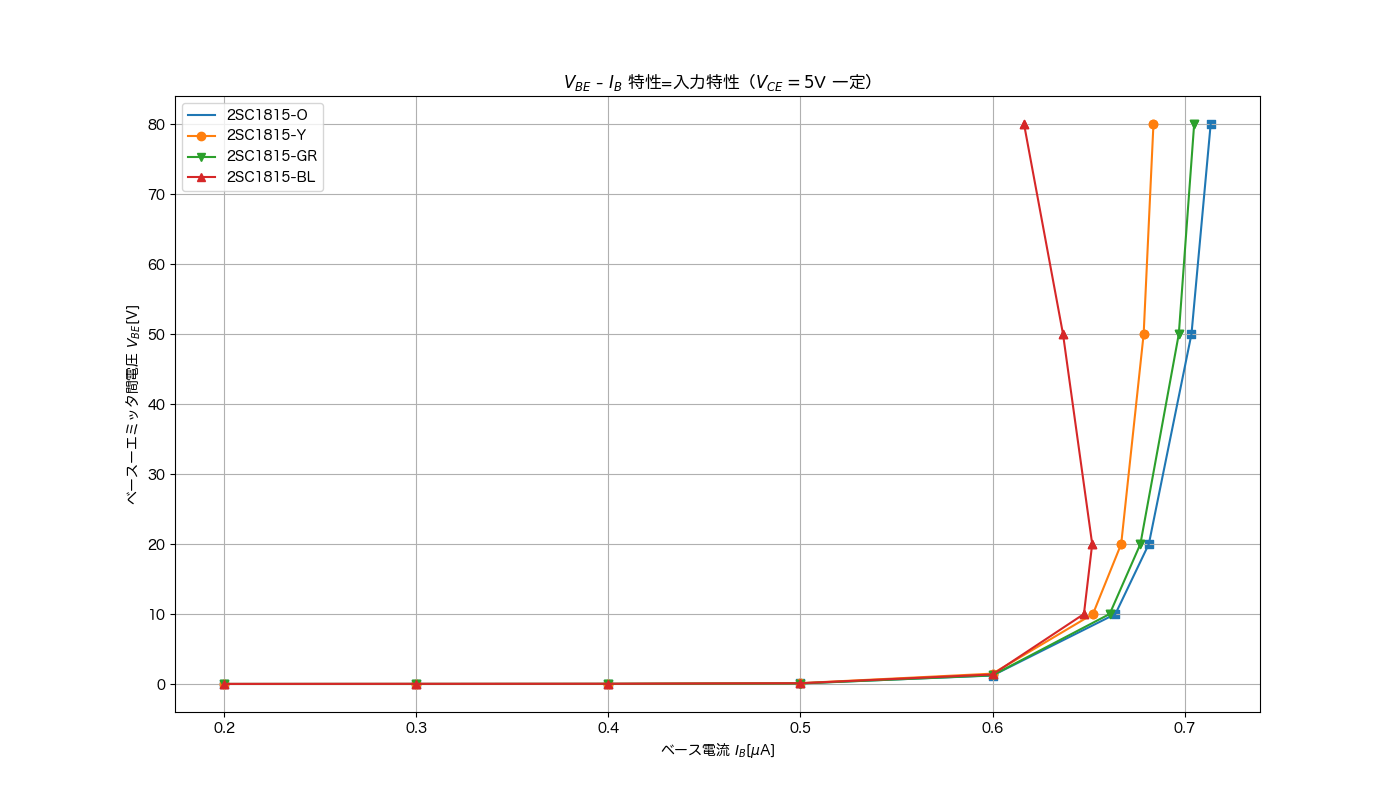
\includegraphics[keepaspectratio, scale=0.48, angle=0]
             {figs/png/staticE03.png}
             \caption{$V_{BE}\;-\;I_B\;$特性}
             \label{fig:ex03}
\end{figure}

\newpage

\subsection{直流負荷線($E_C=9V,\;R_C=390\Omega$):第1象限}

直流負荷線は、トランジスタのコレクタに負荷抵抗$R_C$が接続されている時の、
コレクタ-エミッタ間の電圧$V_{CE}$とコレクタ電流$I_C$の関係を示している

コレクタ電流$I_C$の増加に伴い、コレクタ-エミッタ間の電圧$V_{CE}$は低下する\\

実験の手順は次の通り

\begin{enumerate}
\item[(1)] 負荷抵抗$R_C=390\Omega$を通したコレクタ電流$I_C$を測定できる様に接続を変更する
\item[(2)] ベース電流$I_B=0\;\mu$A になる様に$E_B$を調整し、その状態でコレクタ-エミッタ間の電圧$V_{CE}=9$V となる様に$E_C$を調整する(これ以降$E_C$には触らない)
\item[(3)] コレクタ-エミッタ間の電圧$V_{CE}$を観察しながら、$E_B$(必要に応じて可変抵抗器)を調整して$V_{CE}$を変化させ、その都度コレクタ電流$I_C$測定し記録する  
\end{enumerate}

測定を終えたら、第1象限に直流負荷線を作図する

\vfill

\begin{figure}[H]
  \centering
   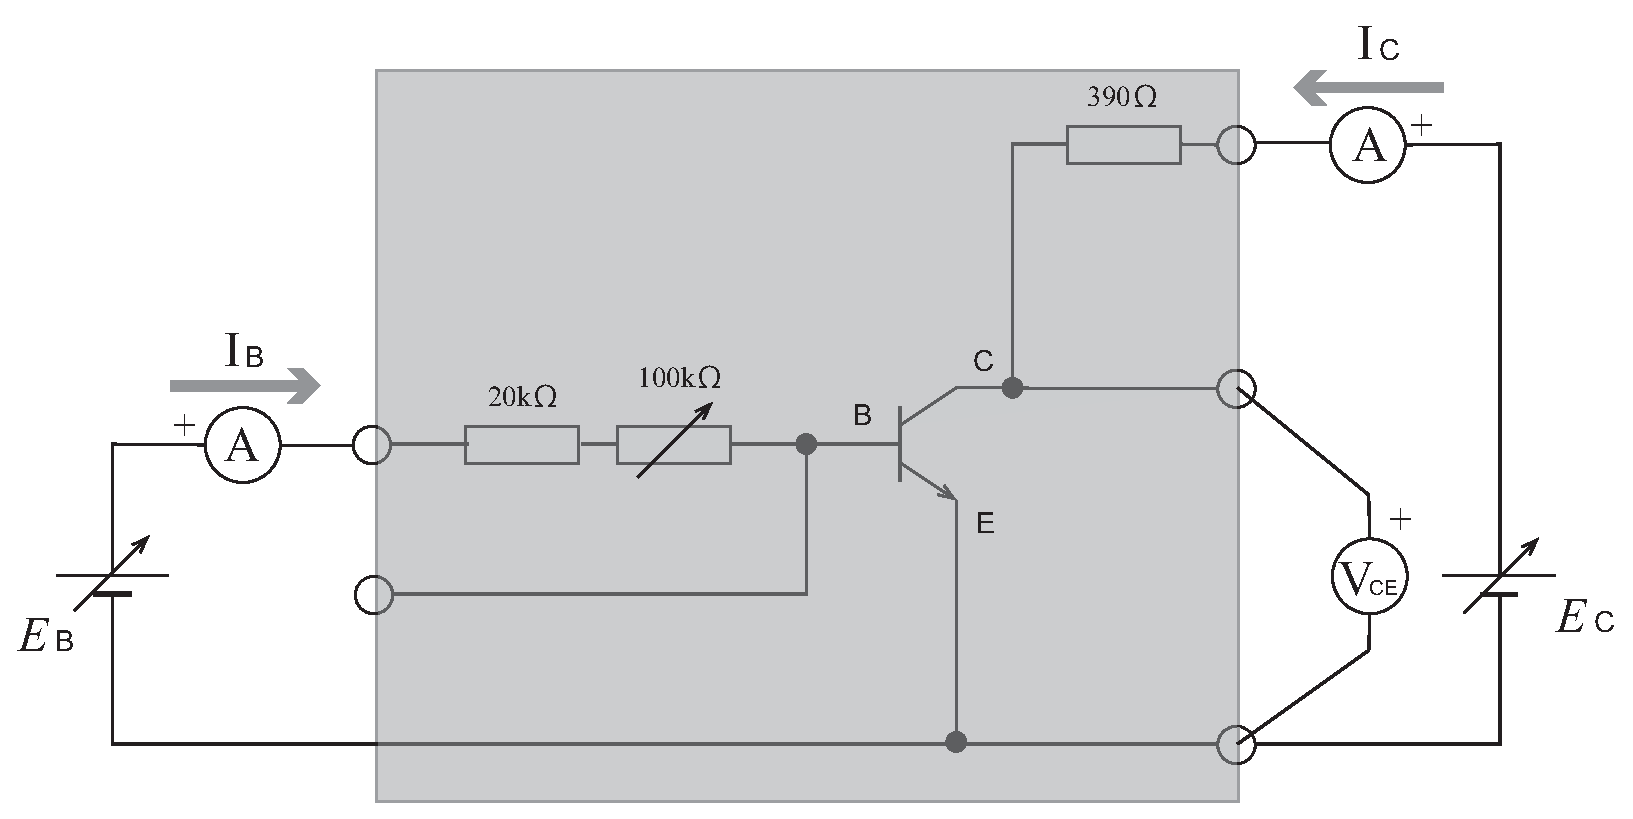
\includegraphics[keepaspectratio, scale=0.5, angle=0]
               {figs/eps/ex4.eps}
               \caption{直流負荷線}
               \label{fig:ex3}
\end{figure}

\vfill

\newpage

\subsubsection{2SC1815Orange}

\begingroup
\renewcommand{\arraystretch}{1.6}
\begin{table}[H]
  \begin{center}
  \caption{2SC1815O:直流負荷線:$E_{C}=9$V、$R_C=390\Omega$}%\label{tbl:t9}\vspace{2mm}
  \begin{tabular}{|r|wr{1cm}|wr{1cm}|wr{1cm}|wr{1cm}|wr{1cm}|wr{1cm}|wr{1cm}|wr{1cm}|wr{1cm}|} \hline
    \multicolumn{1}{|r|}{\cellcolor[rgb]{0.9, 0.9, 0.9}\textbf{$V_{CE}$[V]}} & \multicolumn{1}{c|}{\cellcolor[rgb]{0.9, 0.9, 0.9}\textbf{9.0}} & \multicolumn{1}{c|}{\cellcolor[rgb]{0.9, 0.9, 0.9}\textbf{8.0}} & \multicolumn{1}{c|}{\cellcolor[rgb]{0.9, 0.9, 0.9}\textbf{7.0}} & \multicolumn{1}{c|}{\cellcolor[rgb]{0.9, 0.9, 0.9}\textbf{6.0}} & \multicolumn{1}{c|}{\cellcolor[rgb]{0.9, 0.9, 0.9}\textbf{5.0}} & \multicolumn{1}{c|}{\cellcolor[rgb]{0.9, 0.9, 0.9}\textbf{4.0}} & \multicolumn{1}{c|}{\cellcolor[rgb]{0.9, 0.9, 0.9}\textbf{3.0}} & \multicolumn{1}{c|}{\cellcolor[rgb]{0.9, 0.9, 0.9}\textbf{2.0}} & \multicolumn{1}{c|}{\cellcolor[rgb]{0.9, 0.9, 0.9}\textbf{1.0}}\\ \hline
    \multicolumn{1}{|r|}{\cellcolor[rgb]{0.9, 0.9, 0.9}\textbf{$I_C$[mA]}} & 0 & 2.521 & 5.052 & 7.616 & 10.134 & 12.66 & 15.22 & 17.79 & 20.35 \\ \hline
  \end{tabular}
  \end{center}
\end{table}
\endgroup

\vfill

\subsubsection{2SC1815Yellow}

\begingroup
\renewcommand{\arraystretch}{1.6}
\begin{table}[H]
  \begin{center}
  \caption{2SC1815Y:直流負荷線:$E_{C}=9$V、$R_C=390\Omega$}%\label{tbl:t9}\vspace{2mm}
  \begin{tabular}{|r|wr{1cm}|wr{1cm}|wr{1cm}|wr{1cm}|wr{1cm}|wr{1cm}|wr{1cm}|wr{1cm}|wr{1cm}|} \hline
    \multicolumn{1}{|r|}{\cellcolor[rgb]{0.9, 0.9, 0.9}\textbf{$V_{CE}$[V]}} & \multicolumn{1}{c|}{\cellcolor[rgb]{0.9, 0.9, 0.9}\textbf{9.0}} & \multicolumn{1}{c|}{\cellcolor[rgb]{0.9, 0.9, 0.9}\textbf{8.0}} & \multicolumn{1}{c|}{\cellcolor[rgb]{0.9, 0.9, 0.9}\textbf{7.0}} & \multicolumn{1}{c|}{\cellcolor[rgb]{0.9, 0.9, 0.9}\textbf{6.0}} & \multicolumn{1}{c|}{\cellcolor[rgb]{0.9, 0.9, 0.9}\textbf{5.0}} & \multicolumn{1}{c|}{\cellcolor[rgb]{0.9, 0.9, 0.9}\textbf{4.0}} & \multicolumn{1}{c|}{\cellcolor[rgb]{0.9, 0.9, 0.9}\textbf{3.0}} & \multicolumn{1}{c|}{\cellcolor[rgb]{0.9, 0.9, 0.9}\textbf{2.0}} & \multicolumn{1}{c|}{\cellcolor[rgb]{0.9, 0.9, 0.9}\textbf{1.0}}\\ \hline
    \multicolumn{1}{|r|}{\cellcolor[rgb]{0.9, 0.9, 0.9}\textbf{$I_C$[mA]}} & 0 & 2.555 & 5.057 & 7.567 & 10.118 & 12.65 & 15.21 & 17.75 & 20.30 \\ \hline
  \end{tabular}
  \end{center}
\end{table}
\endgroup

\vfill

\subsubsection{2SC1815GReen}

\begingroup
\renewcommand{\arraystretch}{1.6}
\begin{table}[H]
  \begin{center}
  \caption{2SC1815GR:直流負荷線:$E_{C}=9$V、$R_C=390\Omega$}%\label{tbl:t9}\vspace{2mm}
  \begin{tabular}{|r|wr{1cm}|wr{1cm}|wr{1cm}|wr{1cm}|wr{1cm}|wr{1cm}|wr{1cm}|wr{1cm}|wr{1cm}|} \hline
    \multicolumn{1}{|r|}{\cellcolor[rgb]{0.9, 0.9, 0.9}\textbf{$V_{CE}$[V]}} & \multicolumn{1}{c|}{\cellcolor[rgb]{0.9, 0.9, 0.9}\textbf{9.0}} & \multicolumn{1}{c|}{\cellcolor[rgb]{0.9, 0.9, 0.9}\textbf{8.0}} & \multicolumn{1}{c|}{\cellcolor[rgb]{0.9, 0.9, 0.9}\textbf{7.0}} & \multicolumn{1}{c|}{\cellcolor[rgb]{0.9, 0.9, 0.9}\textbf{6.0}} & \multicolumn{1}{c|}{\cellcolor[rgb]{0.9, 0.9, 0.9}\textbf{5.0}} & \multicolumn{1}{c|}{\cellcolor[rgb]{0.9, 0.9, 0.9}\textbf{4.0}} & \multicolumn{1}{c|}{\cellcolor[rgb]{0.9, 0.9, 0.9}\textbf{3.0}} & \multicolumn{1}{c|}{\cellcolor[rgb]{0.9, 0.9, 0.9}\textbf{2.0}} & \multicolumn{1}{c|}{\cellcolor[rgb]{0.9, 0.9, 0.9}\textbf{1.0}}\\ \hline
    \multicolumn{1}{|r|}{\cellcolor[rgb]{0.9, 0.9, 0.9}\textbf{$I_C$[mA]}} & 0 & 2.473 & 5.085 & 7.511 & 10.083 & 12.62 & 15.18 & 17.69 & 20.24 \\ \hline
  \end{tabular}
  \end{center}
\end{table}
\endgroup

\vfill

\subsubsection{2SC1815BLue}

\begingroup
\renewcommand{\arraystretch}{1.6}
\begin{table}[H]
  \begin{center}
  \caption{2SC1815BL:直流負荷線:$E_{C}=9$V、$R_C=390\Omega$}%\label{tbl:t9}\vspace{2mm}
  \begin{tabular}{|r|wr{1cm}|wr{1cm}|wr{1cm}|wr{1cm}|wr{1cm}|wr{1cm}|wr{1cm}|wr{1cm}|wr{1cm}|} \hline
    \multicolumn{1}{|r|}{\cellcolor[rgb]{0.9, 0.9, 0.9}\textbf{$V_{CE}$[V]}} & \multicolumn{1}{c|}{\cellcolor[rgb]{0.9, 0.9, 0.9}\textbf{9.0}} & \multicolumn{1}{c|}{\cellcolor[rgb]{0.9, 0.9, 0.9}\textbf{8.0}} & \multicolumn{1}{c|}{\cellcolor[rgb]{0.9, 0.9, 0.9}\textbf{7.0}} & \multicolumn{1}{c|}{\cellcolor[rgb]{0.9, 0.9, 0.9}\textbf{6.0}} & \multicolumn{1}{c|}{\cellcolor[rgb]{0.9, 0.9, 0.9}\textbf{5.0}} & \multicolumn{1}{c|}{\cellcolor[rgb]{0.9, 0.9, 0.9}\textbf{4.0}} & \multicolumn{1}{c|}{\cellcolor[rgb]{0.9, 0.9, 0.9}\textbf{3.0}} & \multicolumn{1}{c|}{\cellcolor[rgb]{0.9, 0.9, 0.9}\textbf{2.0}} & \multicolumn{1}{c|}{\cellcolor[rgb]{0.9, 0.9, 0.9}\textbf{1.0}}\\ \hline
    \multicolumn{1}{|r|}{\cellcolor[rgb]{0.9, 0.9, 0.9}\textbf{$I_C$[mA]}} & 0.0 & 2.489 & 5.089 & 7.595 & 10.144 & 12.70 & 15.26 & 17.83 & 20.38 \\ \hline
  \end{tabular}
  \end{center}
\end{table}
\endgroup

\newpage

\begin{figure}[H]
  \centering
   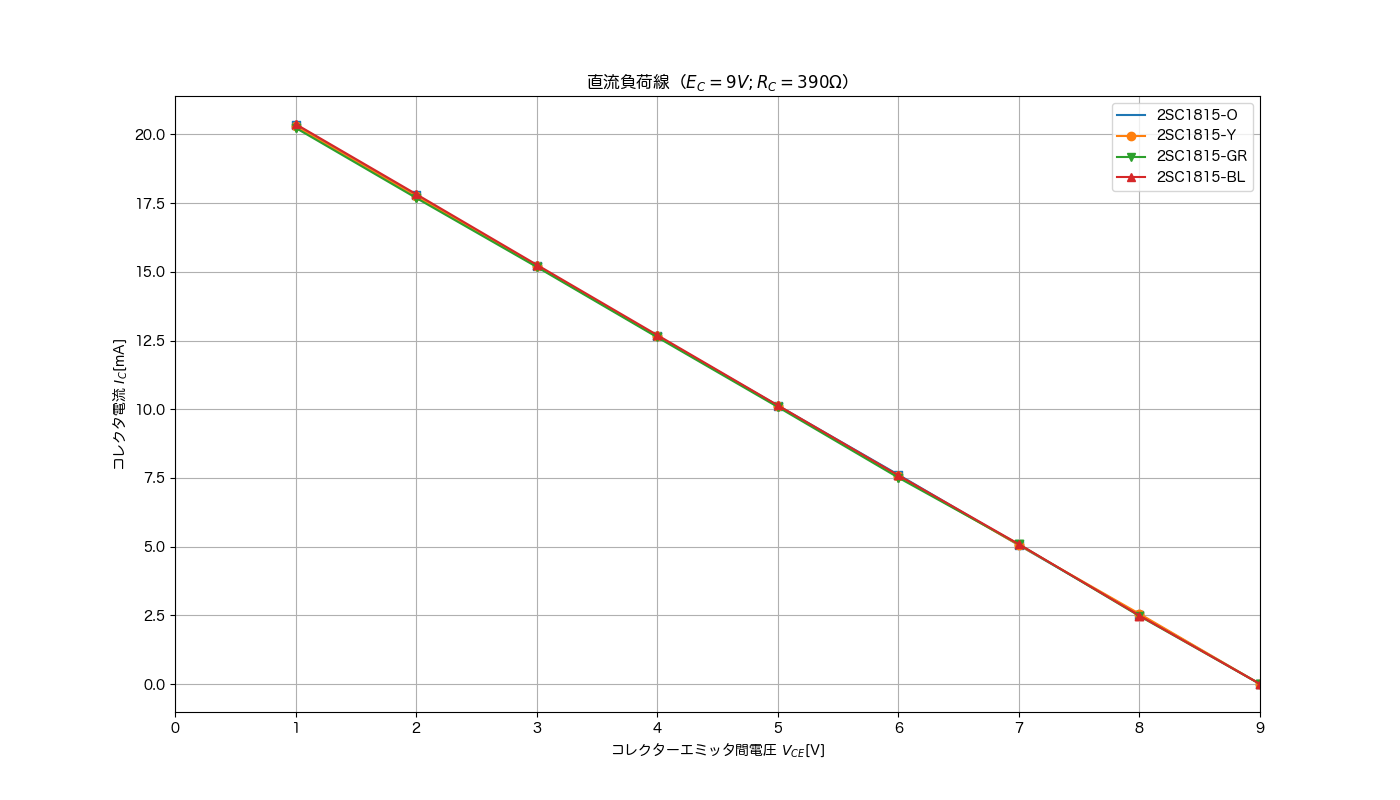
\includegraphics[keepaspectratio, scale=0.48, angle=0]
             {figs/png/staticE04.png}
             \caption{直流負荷線}
             \label{fig:ex04}
\end{figure}

\newpage

\begin{figure}[H]
     \centering
      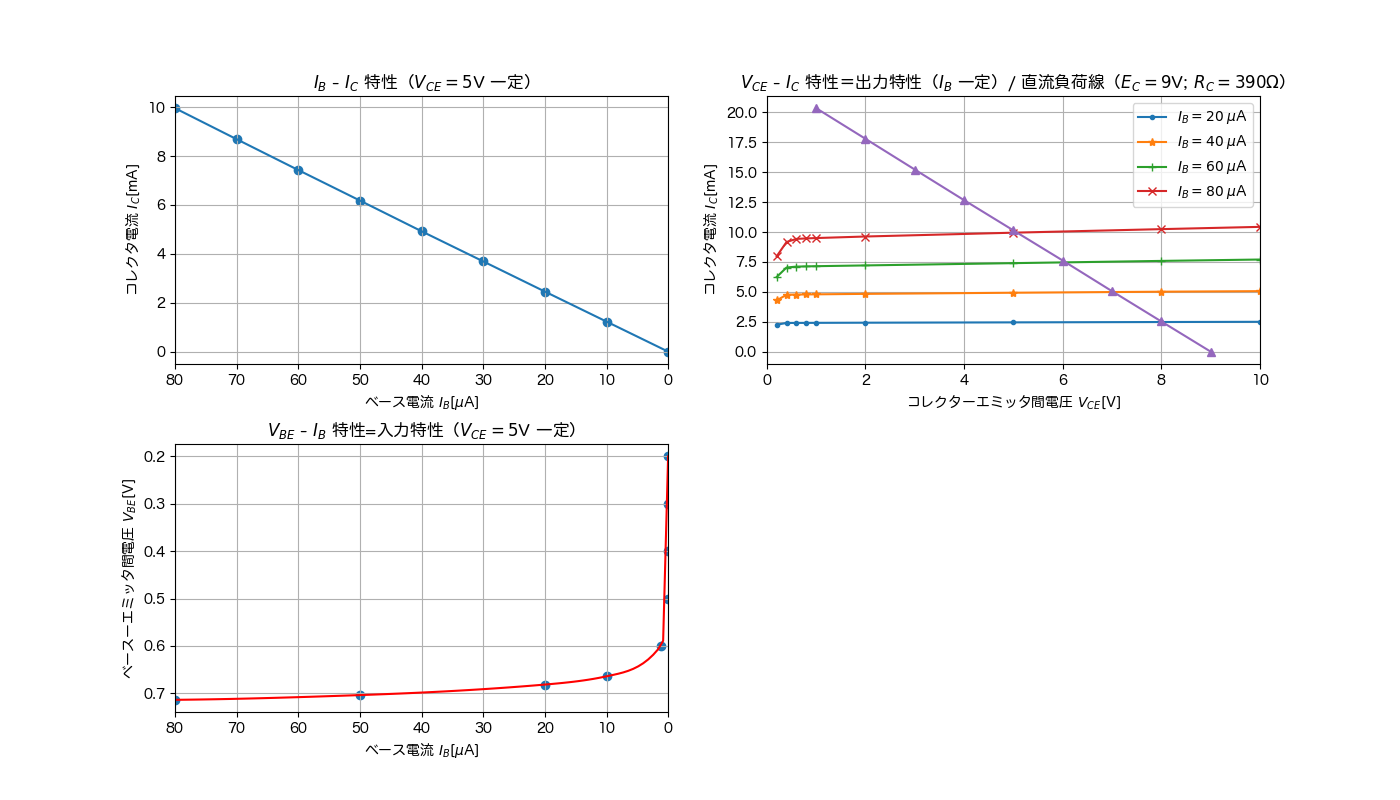
\includegraphics[keepaspectratio, scale=0.65, angle=90]
                  {figs/png/staticO.png}
                  \caption{2SC1815O}
                  \label{fig:o}
\end{figure}

\begin{figure}[H]
     \centering
      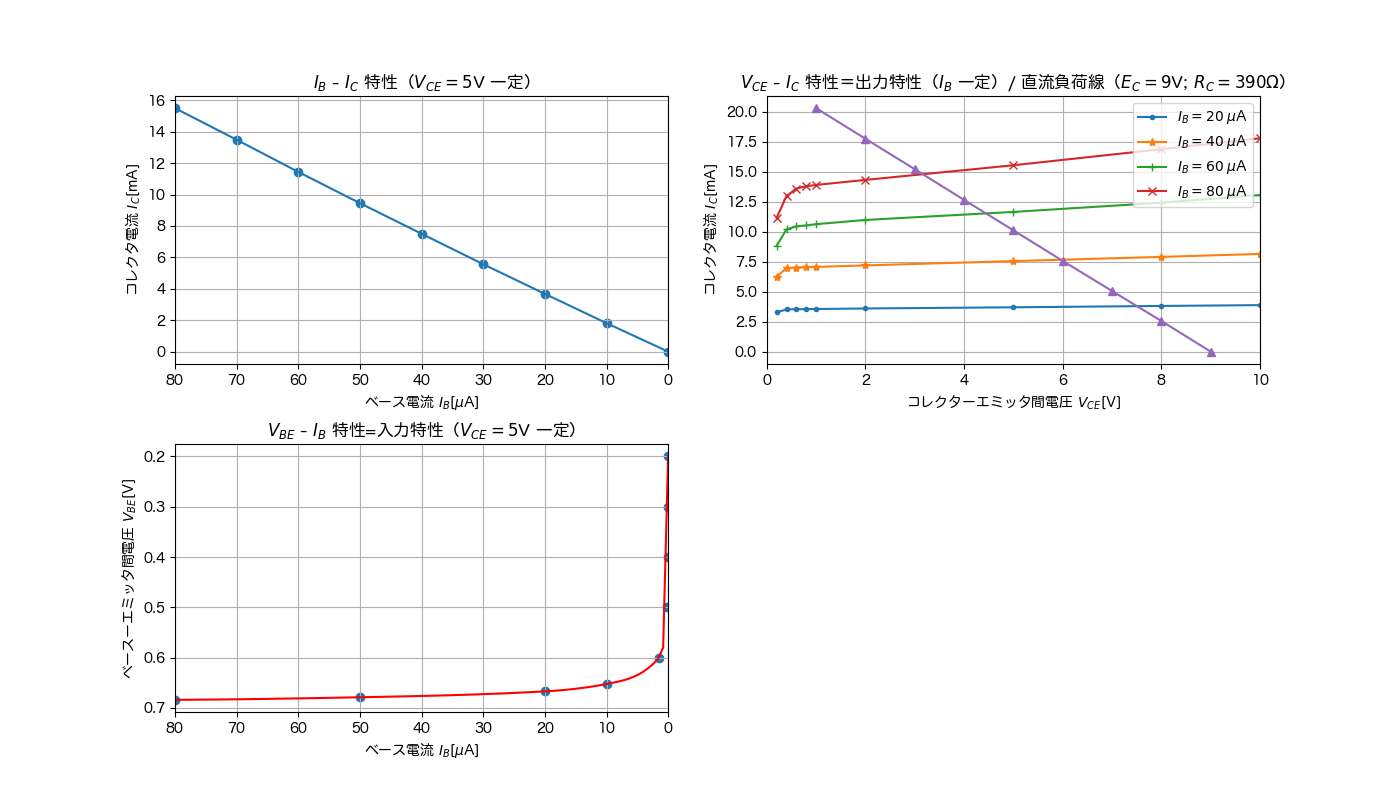
\includegraphics[keepaspectratio, scale=0.65, angle=90]
                {figs/png/staticY.png}
                \caption{2SC1815Y}
                \label{fig:y}
\end{figure}

\begin{figure}[H]
    \centering
     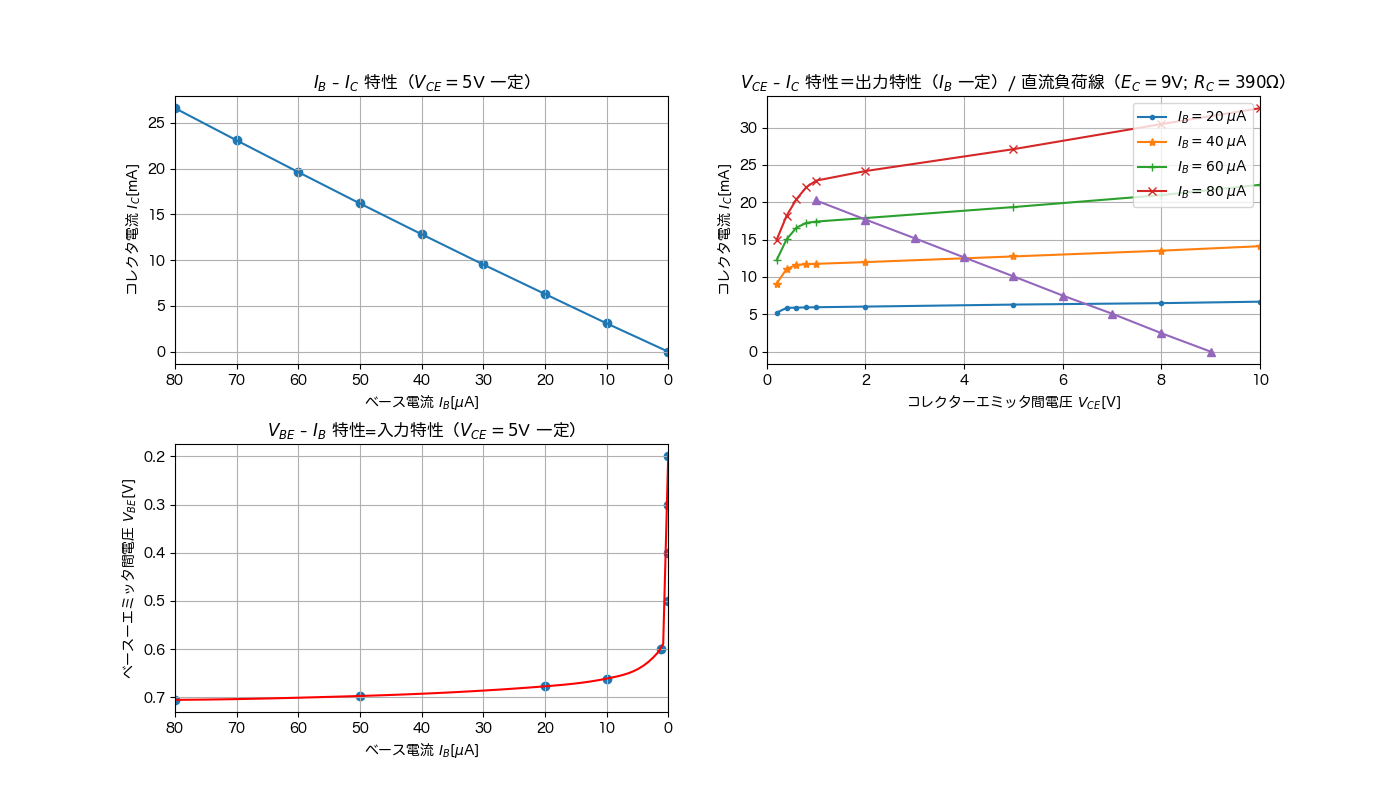
\includegraphics[keepaspectratio, scale=0.65, angle=90]
                 {figs/png/staticG.png}
                 \caption{2SC1815GR}
                 \label{fig:gr}
\end{figure}

\begin{figure}[H]
    \centering
     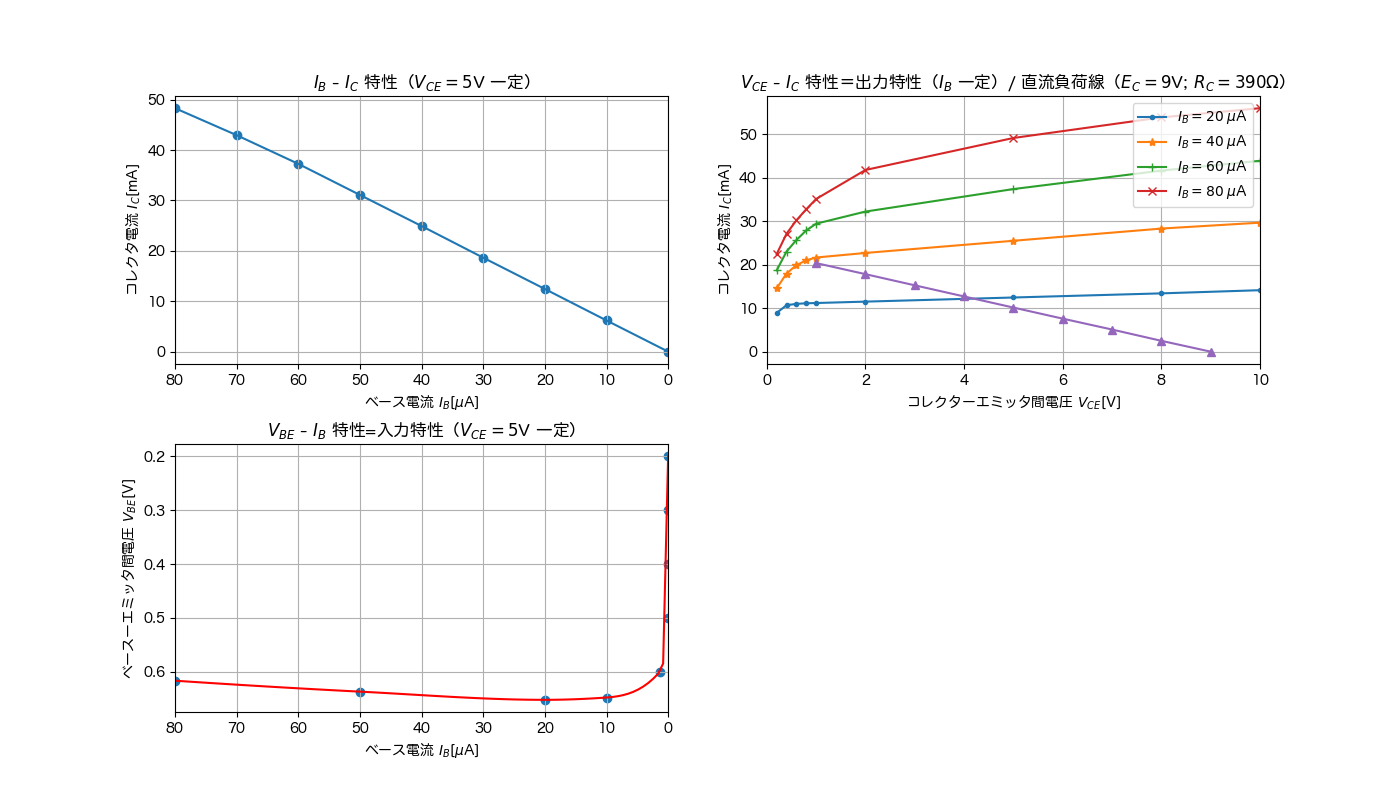
\includegraphics[keepaspectratio, scale=0.65, angle=90]
               {figs/png/staticB.png}
               \caption{2SC1815BL}
               \label{fig:b}
\end{figure}

\newpage

%\newpage

\section{製作・実験 ②:周波数特性}


\subsection{電流帰還バイアス回路設計の手順}

\begin{enumerate}
\item まず$R_E$を決める\footnote{実教の教科書「電子回路」(第2章第5節)小信号増幅回路の設計より}
\begin{enumerate}
\item[(1)] コレクタ電流$I_C$として$1$mA を流すことにする(設計条件)
\item[(2)] エミッタ抵抗での電圧降下$V_E$は、$V_{CC}=12V$の$10\%$になる様にする(設計条件)\\そうすると、$V_{RE}=1.2V$
\item[(3)] $I_E=I_B+I_C$だが、実際には$I_B\ll I_C$であることから、$I_E\fallingdotseq I_C$と概算することにして、\\
$R_E$にも$I_C$と同じ$I_E=1mA$が流れると考えれば、その時の電圧降下が$V_{RE}=1.2V$なのだから、$R_E=\displaystyle\frac{1.2}{1\times 10^3}=1.2k\Omega$
\item[(4)] $1.2\;k\Omega$はE系列\footnote{抵抗値と静電容量値には、いくつかの標準数列が規定され、推奨されている。標準数列のE24系列の数値は次の通り。\\
$1.0\;\;1.1\;\;1.2\;\;1.3\;\;1.5\;\;1.6\;\;1.8\;\;2.0\;\;2.2\;\;2.4\;\;2.7\;\;3.0\;\;3.3\;\;3.6\;\;3.9\;\;4.3\;\;4.7\;\;5.1\;\;5.6\;\;6.2\;\;6.8\;\;7.5\;\;8.2\;\;9.1$}
にある数値なので、$R_E=1.2\;k\Omega$とする
\end{enumerate}
\vfill
\item 次に、$R_C$を決める
\begin{enumerate}
\item[(1)] $V_{CE}\fallingdotseq V_{RC}$となる様にすれば、最大値の大きな交流信号を出力できる様になるので、\\
$V_{CC}=V_{RC}+V_{CE}+V_{RE}$において、$V_{CE}=V_{RC}$とおけば、
$V_{RC}=\displaystyle\frac{V_{CC}-V_{RE}}{2}$
\item[(2)] 設計条件より$I_C=1mA$だったから、$R_C=\displaystyle\frac{V_{RC}}{I_C}=\frac{V_{CC}-V_{RE}}{2I_C}=\frac{12-1.2}{2\times 1\times 10^{-3}}=5.4k\Omega$
\item[(3)] E系列から、$R_C=5.6k\Omega$を選ぶ
\end{enumerate}
\vfill
\item ブリーダ抵抗$R_A$を決める
\begin{enumerate}
\item[(1)] $h_{FE}\fallingdotseq 180$のトランジスタを使うことを想定している(設計条件)ので、\\
コレクタ電流$I_C$に$1mA$を流す時のベース電流$I_B$は、
$I_B=\displaystyle\frac{I_C}{h_{FE}}=\frac{1\times 10^{-3}}{180}=5.6\mu A$
\item[(2)] $R_A$にはベース電流$I_B$の20倍の電流を流すことにする(設計条件)と、$I_A=20\times I_B=112\mu A$
%\item[(3)] $R_B$に流れる電流$I_B$は、$R_A$に流れる電流$I_A$とベースに流れる電流$I_B$の和になる
\item[(3)] ベース電位は$V_B=V_{BE}+V_{RE}$であり、$I_C=1mA$の時の$V_{BE}$を、シリコントランジスタの一般的な値である$0.6V$にとれば、
$V_B=V_{RE}+V_{BE}=1.2+0.6=1.8V$
\item[(4)] この値$V_B$は、$R_A$にブリーダ電流$I_A$が流れることによる電圧降下$V_{RA}$に等しいから、\\
$R_A=\displaystyle\frac{V_{RA}}{I_A}=\frac{V_B}{I_A}=\frac{1.8}{112\times 10^{-6}}=16.1\fallingdotseq 16\;k\Omega$
\item[(5)] $16\;k\Omega$はE系列にある数値なので、このまま$R_A=16\;k\Omega$
\end{enumerate}
\vfill
\item 最後に、$R_B$を決める
\begin{enumerate}
\item[(1)] ブリーダ抵抗$R_A$と$R_B$は$V_{CC}$を分圧しているので、
$V_{RB}=V_{CC}-V_{RA}=12-1.8=10.2V$
\item[(2)] $R_B$にはブリーダ電流$I_A$とベース電流$I_B$の両方$I_A+I_B$が流れるので、
$V_{RB}=R_B\cdot(I_A+I_B)$\\
従って$R_B=\displaystyle\frac{V_{RB}}{I_A+I_B}=\frac{10.2}{112\times 10^{-6}+5.6\times 10^{-6}}=86.7\times 10^3\fallingdotseq 87k\Omega$
\item[(3)] E系列から$R_B=91k\Omega$を選ぶが、コレクタ電流を$I_C=1mA$に調整できる様にするため、\\
$R_B$には、E系列の$68k\Omega$に半固定抵抗の$50k\Omega$を直列に接続することも考えられる
\end{enumerate}
\end{enumerate}

\vfill

\begin{comment}
\begin{enumerate}
\item $R_E=\displaystyle\frac{V_{RE}}{I_E}=\frac{0.1 V_{CC}}{I_E}=1.2k\Omega$\quad$\because V_{RE}=0.1V_{CC},\;I_E=I_B+I_C\fallingdotseq I_C=1mA,\;I_B\ll I_C$
\item $R_C=\displaystyle\frac{V_{CC}-V_E}{2I_C}=5.4k\Omega$\quad $\because V_{RC}=R_C I_C,\;V_{RC}=\displaystyle\frac{V_{CC}-V_E}{2},\;V_{CC}=V_{RC}+V_{CE}+V_{E}$
\item $I_A=20 I_B=112\mu A$\quad$\because I_B=\displaystyle\frac{I_C}{h_{FE}}\fallingdotseq 5.6\mu A,\;h_{FE}=180,\;I_C=1mA$
\item $V_B=V_{RA}=V_E+V_{BE}=0.1V_{CC}+V_{BE}=1.2+0.6=1.8V$
\item $V_{RB}=V_{CC}-V_{RA}=V_{CC}-V_B=12-1.8=10.2V$\quad $\because V_{CC}=V_{RA}+V_{RB},\;V_{RA}=V_B$
\item $R_A=\displaystyle\frac{V_B}{I_A}\fallingdotseq 16k\Omega$\quad $\because V_{RA}=V_B=V_{CC}-V_{RB}=R_A I_A=1.8V$
\item $R_B=\displaystyle\frac{V_{RB}}{I_A+I_B}\fallingdotseq 87k\Omega$\quad $\because V_{RB}=R_B(I_A+I_B)=10.2V$
\end{enumerate}
\end{comment}

\newpage

\begin{multicols}{2}
  \begin{figure}[H]
     \centering
      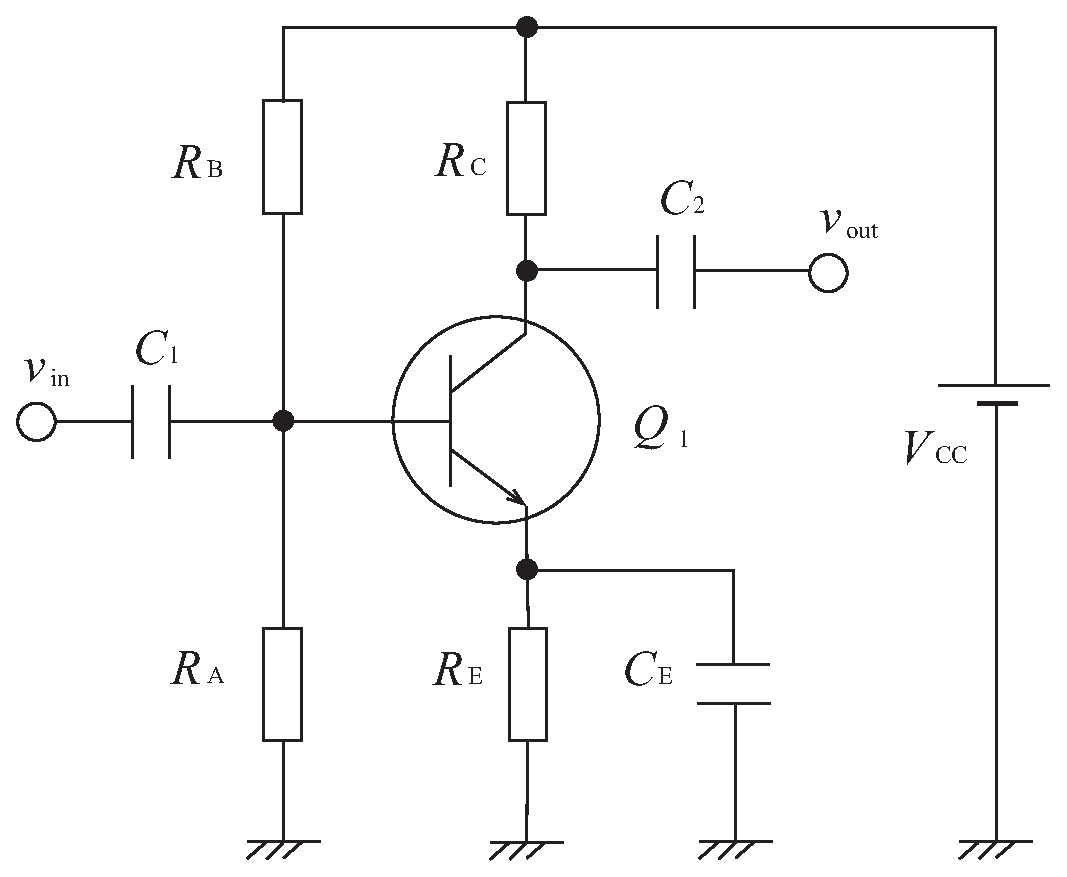
\includegraphics[keepaspectratio, scale=0.3, angle=0]
                  {figs/eps/exp1.eps}
                  \caption{小信号増幅回路の製作}
                  \label{fig:8_1}
  \end{figure}

  \begin{figure}[H]
     \centering
      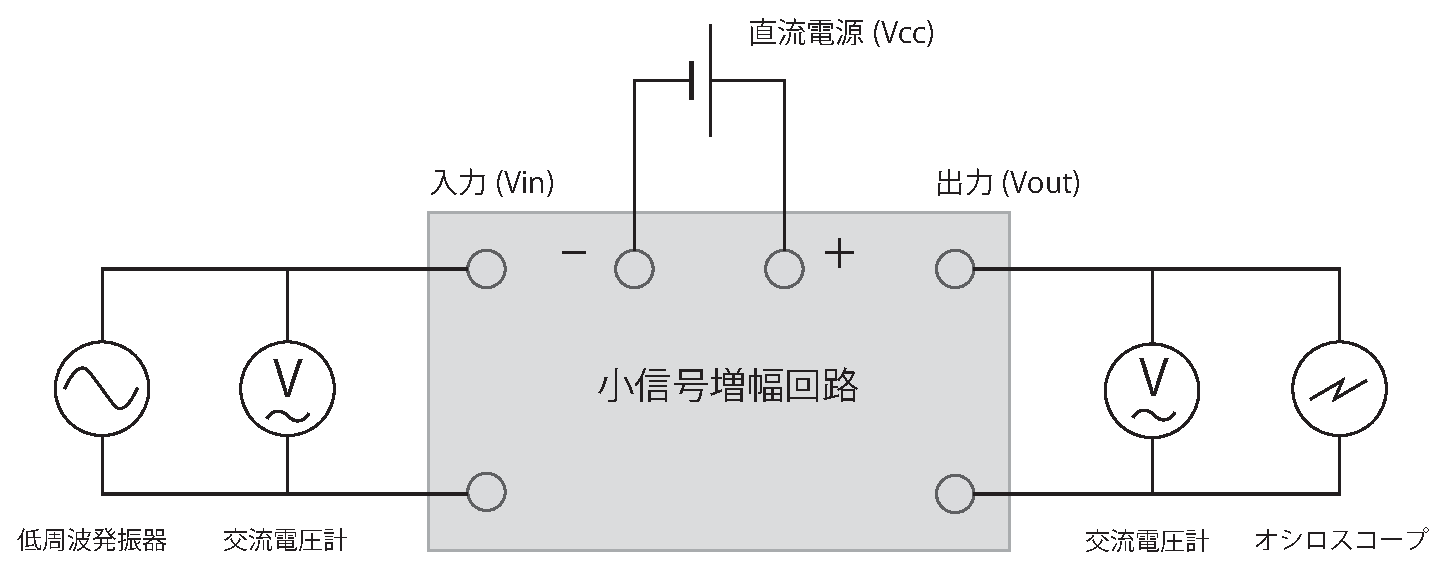
\includegraphics[keepaspectratio, scale=0.3, angle=0]
                {figs/eps/sokutei.eps}
                \caption{実験装置の構成}
                \label{fig:8_2}
  \end{figure}
\end{multicols}

%使用トランジスタの$h_{FE}$\footnote{回路計による実測値} : O=117、 Y=187、 GR=258、 BL=597

\subsection{教科書の回路モデルの製作}

\begin{table}[H]
\begin{center}
\caption{実教「電子回路」P99より}
\begin{tabular}{|c|l|l|l|l|} \hline
  \multicolumn{1}{|c|}{\textbf{項番}} & \multicolumn{1}{c|}{\textbf{項目}} & \multicolumn{1}{c|}{\textbf{属性}} & \multicolumn{1}{c|}{\textbf{表記}} & \multicolumn{1}{c|}{\textbf{備考}} \\ \hline
  1 & 半固定抵抗器($R_E$) & 〜$2\;k\Omega$($1.2\;k\Omega$) & 202 & $20\times 10^2\Omega$,直線性B \\
  2 & 抵抗器($R_C$) & $5.6\;k\Omega$ & 緑・青・赤 & $56\times 10^2\Omega$ \\
  3 & 抵抗器($R_{A}$) & $16\;k\Omega$ & 茶・青・橙 & $16\times 10^3\Omega$ \\
  4 & 抵抗器($R_{B}$) & $91\;k\Omega$ & 白・茶・橙 & $91\times 10^3\Omega$ \\
  5 & 電解コンデンサ($C_1$) & $10\;\mu$F、16V & & 結合コンデンサ \\
  6 & 電解コンデンサ($C_2$) & $10\;\mu$F、16V & & 結合コンデンサ \\
  7 & 電解コンデンサ($C_E$) & $330\;\mu$F、16V & & バイパスコンデンサ \\
  8 & トランジスタ($Q_1$) & npn、 $h_{FE}\fallingdotseq180$ & 2SC1815\footnotemark & エミッタ接地 \\ \hline
  9 & 直流電源($V_{CC}$) & DC 12V & DK-910 & Sunhayato \\
  10 & 発振器($V_{in}$) & 正弦波、10Hz〜1MHz & AG-204D & KENWOOD \\
  11 & AC電圧計($V_{in}$、$V_{out}$) & $V_{in}$は5mV(実効値)に & VT-187 & KENWOOD \\
  12 & オシロスコープ & CH1:$V_{in}$、CH2:$V_{out}$ & DS1054Z & RIGOL \\ \hline
\end{tabular}
\end{center}
\end{table}
\footnotetext{教科書では$h_{FE}\fallingdotseq 180$とされていることから、トランジスタには2SC1815Yの使用を想定している様に見える}

\subsection{LTspiceによるシミュレーション}

2SC1815Yを想定して周波数応答のシミュレーションを実施した。\\
以下のSPICE directiveを使った。(教科書では$R_E=1.2k\Omega$になっている)
\begin{verbatim}
  .ac dec 50 10 1MEG
  .step param R list 0.4k 0.46k 1.2k
\end{verbatim}

シミュレーションの結果と実機による測定データの間で、特に高域遮断周波数に乖離を生じることについて、
「実機では信号ケーブルと計測器の入力インピーダンスが加わるのが原因である」\footnote{トラ技SPECIAL「設計のためのLTspice回路解析101選」第1部第1章
「シミュレーション回路を実機に近づける」}ので、
ケーブルを含めた容量$85pF$と入力抵抗$1M\Omega$(オシロスコープのプローブが$\times 1$の場合)
を基本モデルに追加してシミュレーションをやり直し、実機に合わせるようにしてみた。\\

なお、LTspiceの標準ライブラリでは2SC1815を選べないので、
以下の様にしてポピュラーなトランジスタのデータを追加する操作をした。
\footnote{\url{https://qiita.com/exabugs/items/5bfb3a575ce05bb6cbde}}

LTSpiceの標準ライブラリの所在は、
\begin{verbatim}
  ~/Library/Application\ Support/LTspice/lib
\end{verbatim}
このフォルダの下には3つのフォルダがあって、それぞれのファオルダは次の様になっている。
\begin{table}[H]
  \begin{center}
  \caption{LTspiceライブラリの構成}
  \begin{tabular}{|c|l|} \hline
    \multicolumn{1}{|c|}{\textbf{フォルダ}} & \multicolumn{1}{c|}{\textbf{内容}} \\ \hline\hline
    cmp & ダイオードやトランジスタなどのパラメータ・モデルのデータ・ファイル \\ \hline
    sub & デバイスの回路情報がセットされたlibファイルやsubファイル \\ \hline
    sym & 回路図を作成する時のデバイスのシンボルのデータ \\ \hline
  \end{tabular}
  \end{center}
\end{table}
トランジスタはcmpフォルダに置かれることになっている様なので、
このcmpフォルダの中のファイル standard.bjt の最後に以下を追記する。(テキストエディタで編集可)

\begin{verbatim}
  *Low Noise Amp PC=0.4W Ic=0.15A Vcbo=60V Complementary 2SA1015
  .model 2SC1815 NPN(Is=2.04E-15 Xti=3 Eg=1.11 Vaf=100 Bf=300 Ne=1.5 Ise=0
  + Vceo=50 Icrating=150m mfg=TOSHIBA
  + Ikf=200m Xtb=1.5 Br=3.377 Nc=2 Isc=0 Ikr=0 Rc=1 Cjc=1p Mjc=.3333
  + Vjc=.75 Fc=.5 Cje=25p Mje=.3333 Vje=.75 Tr=450n Tf=20n Itf=0 Vtf=0 Xtf=0)
  
  .model 2SC1815-GR NPN(Is=2.04E-15 Xti=3 Eg=1.11 Vaf=100 Bf=300 Ne=1.5 Ise=0
  + Vceo=50 Icrating=150m mfg=TOSHIBA
  + Ikf=200m Xtb=1.5 Br=3.377 Nc=2 Isc=0 Ikr=0 Rc=1 Cjc=1p Mjc=.3333
  + Vjc=.75 Fc=.5 Cje=25p Mje=.3333 Vje=.75 Tr=450n Tf=20n Itf=0 Vtf=0 Xtf=0)
  
  .model 2SC1815-Y NPN(Is=2.04E-15 Xti=3 Eg=1.11 Vaf=100 Bf=200 Ne=1.5 Ise=0
  + Vceo=50 Icrating=150m mfg=TOSHIBA
  + Ikf=200m Xtb=1.5 Br=3.377 Nc=2 Isc=0 Ikr=0 Rc=1 Cjc=1p Mjc=.3333
  + Vjc=.75 Fc=.5 Cje=25p Mje=.3333 Vje=.75 Tr=450n Tf=20n Itf=0 Vtf=0 Xtf=0)
  
  *Low Noise Amp PC=0.4W Ic=0.15A Vcbo=50V Complementary 2SC1815
  .model 2SA1015 PNP(Is=295.1E-18 Xti=3 Eg=1.11 Vaf=100 Bf=300 Ne=1.5 Ise=0
  + Vceo=50 Icrating=150m mfg=TOSHIBA
  + Ikf=200m Xtb=1.5 Br=10.45 Nc=2 Isc=0 Ikr=0 Rc=15 Cjc=66.2p
  + Mjc=1.054 Vjc=.75 Fc=.5 Cje=5p Mje=.3333 Vje=.75 Tr=10n Tf=1.661n Itf=0 Vtf=0 Xtf=0)
  
  .model 2SA1015-GR PNP(Is=295.1E-18 Xti=3 Eg=1.11 Vaf=100 Bf=300 Ne=1.5 Ise=0
  + Vceo=50 Icrating=150m mfg=TOSHIBA
  + Ikf=200m Xtb=1.5 Br=10.45 Nc=2 Isc=0 Ikr=0 Rc=15 Cjc=66.2p
  + Mjc=1.054 Vjc=.75 Fc=.5 Cje=5p Mje=.3333 Vje=.75 Tr=10n Tf=1.661n Itf=0 Vtf=0 Xtf=0)
  
  .model 2SA1015-Y PNP(Is=295.1E-18 Xti=3 Eg=1.11 Vaf=100 Bf=200 Ne=1.5 Ise=0
  + Vceo=50 Icrating=150m mfg=TOSHIBA
  + Ikf=200m Xtb=1.5 Br=10.45 Nc=2 Isc=0 Ikr=0 Rc=15 Cjc=66.2p
  + Mjc=1.054 Vjc=.75 Fc=.5 Cje=5p Mje=.3333 Vje=.75 Tr=10n Tf=1.661n Itf=0 Vtf=0 Xtf=0)  
\end{verbatim}

このライブラリデータの根拠となるデータシートの所在は次の通り\\
\url{http://akizukidenshi.com/download/2sc1815-gr.pdf}\\
\url{http://akizukidenshi.com/download/2sa1015-gr.pdf}\\

\begin{spacing}{0.2}
  %\begin{multicols}{2}
  \begin{figure}[H]
    \centering
     \includegraphics[keepaspectratio, scale=0.19, angle=0]
                 {figs/jpg/DSC_0285.jpg}
                 \caption{実習装置}
                 \label{fig:pic1}
 \end{figure}

 \begin{figure}[H]
    \centering
     \includegraphics[keepaspectratio, scale=0.193, angle=0]
               {figs/jpg/DSC_0295x.jpg}
               \caption{周波数特性の測定}
               \label{fig:pic2}
 \end{figure}
  %\end{multicols}
\end{spacing}

\newpage

%\begin{spacing}{0.67}
%  \begin{multicols}{2}
    \begin{figure}[H]
       \centering
        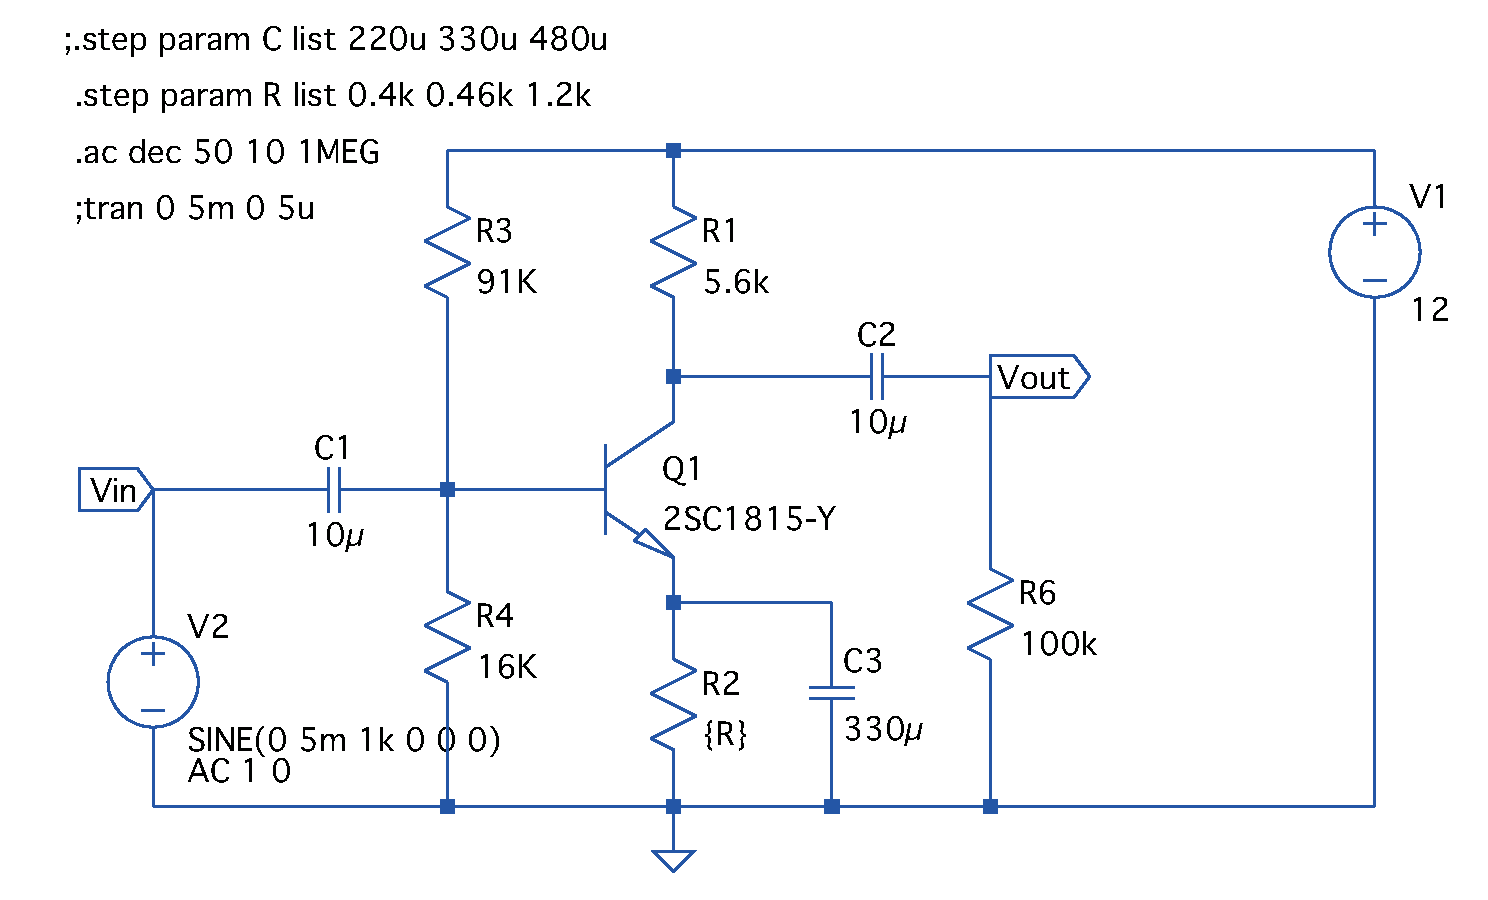
\includegraphics[keepaspectratio, scale=0.65, angle=0]
                    {figs/eps/kyokasyoM1Yalt.eps}
                    \caption{LTSpiceによるモデル化}
                    \label{fig:spice1}
    \end{figure}
  
    \begin{figure}[H]
       \centering
        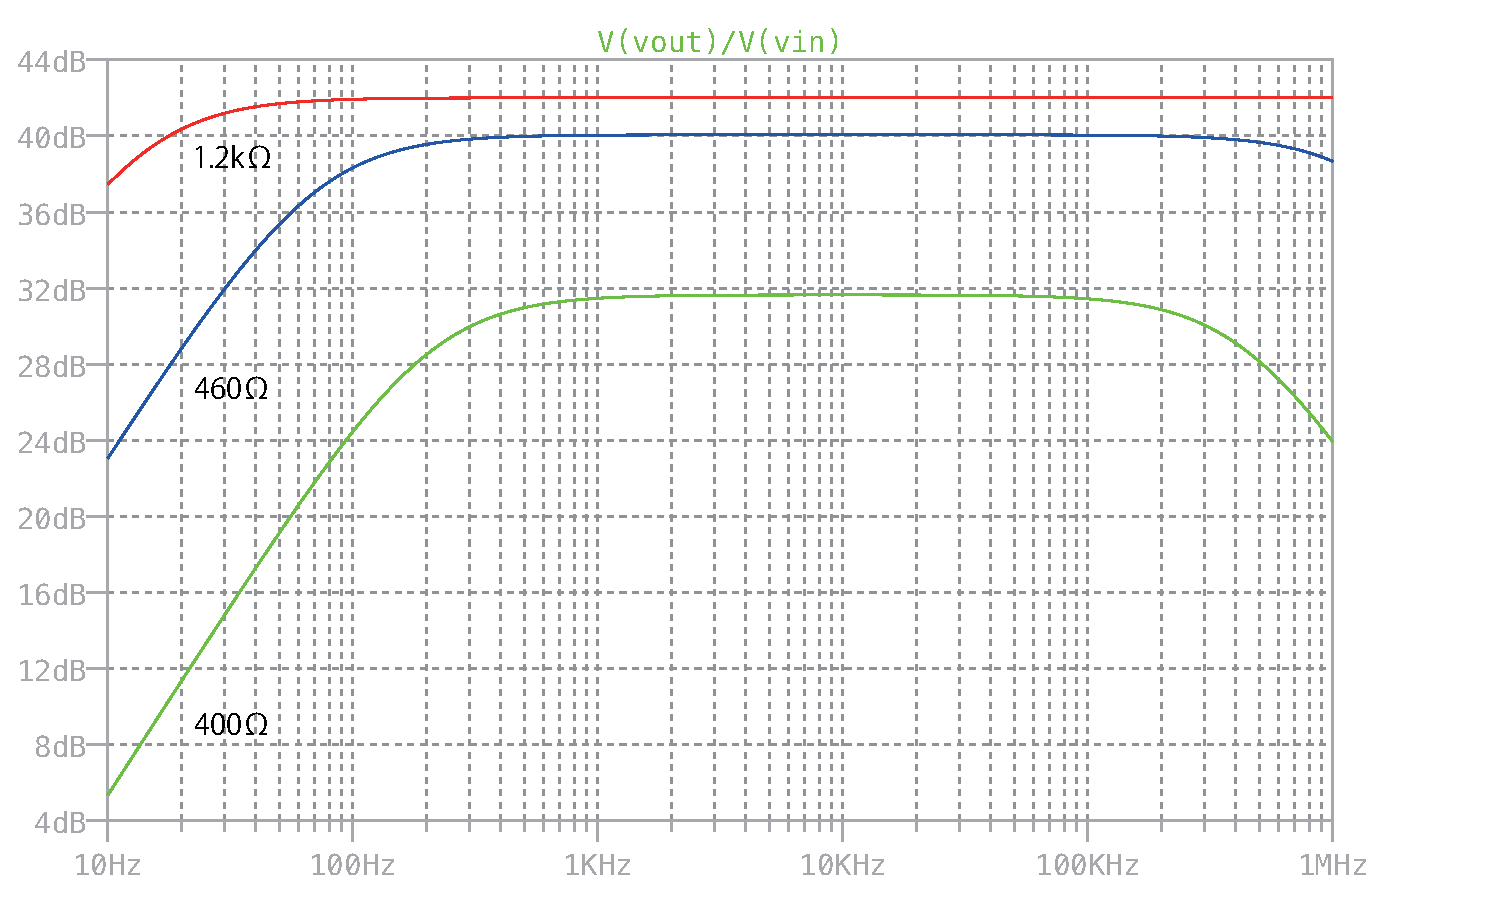
\includegraphics[keepaspectratio, scale=0.65, angle=0]
                  {figs/eps/_kyokasyoM1YaltFrqs.eps}
                  \caption{$R_E=1.2k\Omega$の特性が$f=1MHz$になってもフラットなままだが}
                  \label{fig:spice2}
    \end{figure}
%  \end{multicols}
%\end{spacing}

%\begin{spacing}{0.67}
%  \begin{multicols}{2}
    \begin{figure}[H]
       \centering
        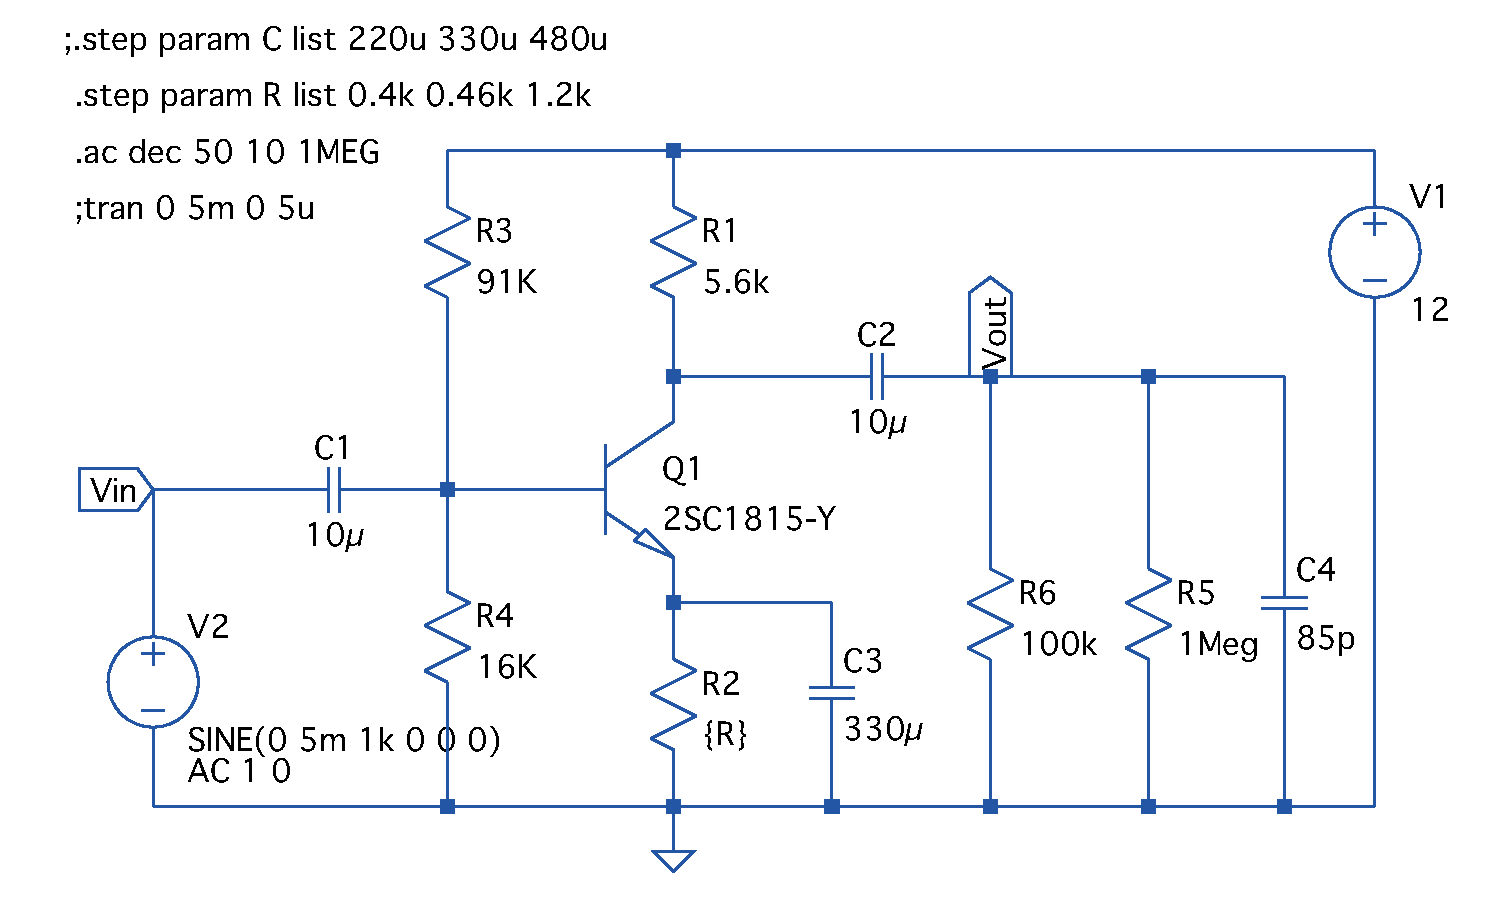
\includegraphics[keepaspectratio, scale=0.65, angle=0]
                    {figs/eps/kyokasyoM1Y.eps}
                    \caption{出力に、計測器とケーブルのCR(R5とC4)を追加して実機に合わせた}
                    \label{fig:spice3}
    \end{figure}
  
    \begin{figure}[H]
       \centering
        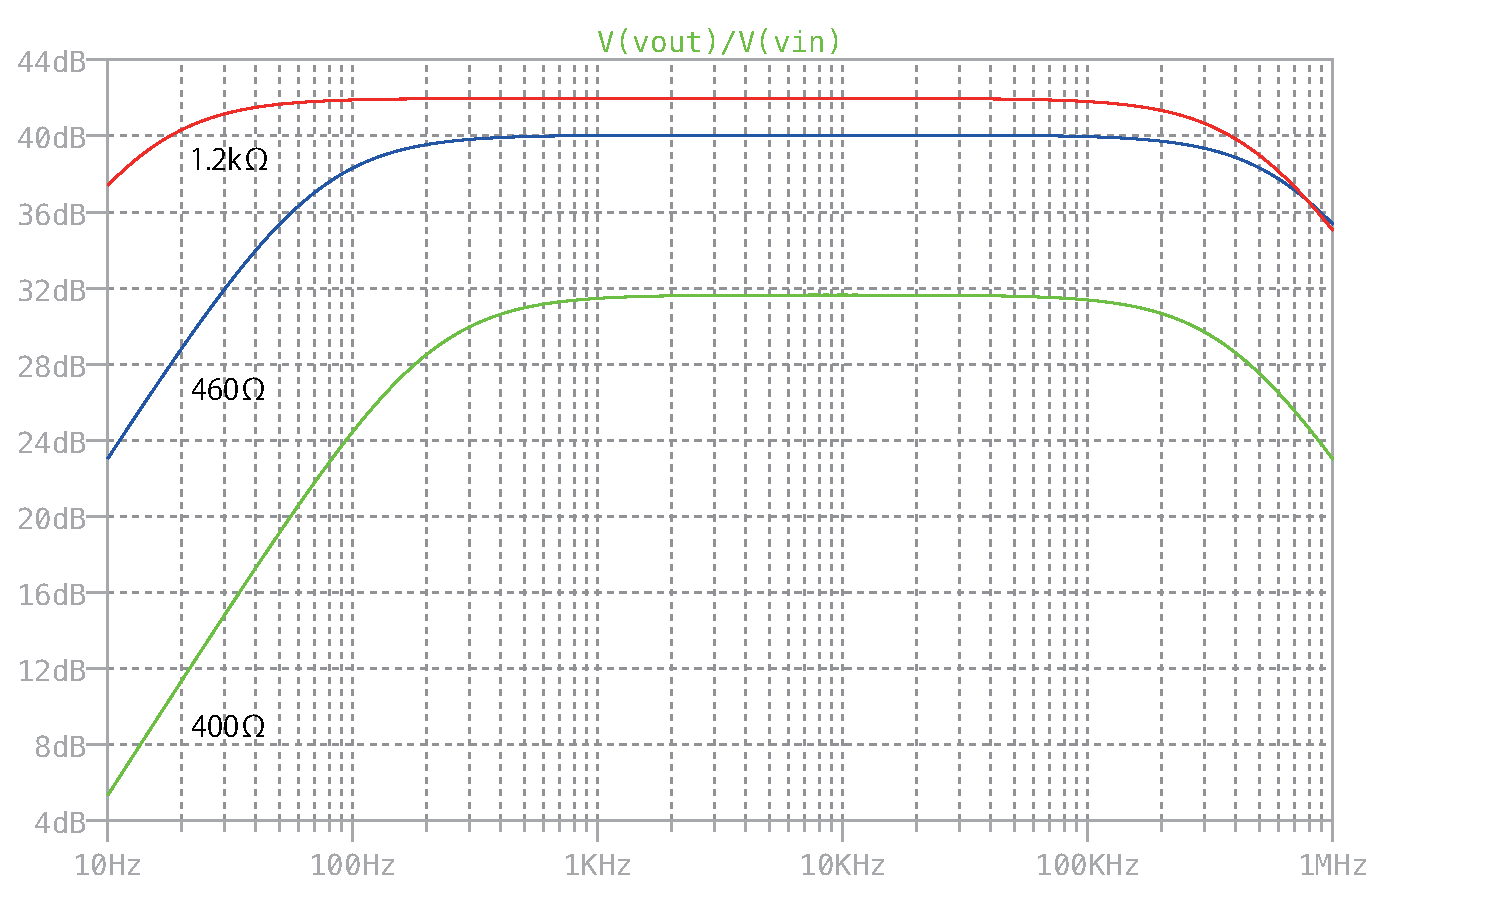
\includegraphics[keepaspectratio, scale=0.65, angle=0]
                  {figs/eps/_kyokasyoM1YFrqs.eps}
                  \caption{$R_E=1.2k\Omega$の特性が$f=100kHz$辺りから右肩が下がってきている}
                  \label{fig:spice4}
    \end{figure}
%  \end{multicols}
%\end{spacing}

\newpage

\subsection{実測データ:2SC1815Y}

%\vspace{-2mm}
\begin{table}[H]
  \begin{center}
  \caption{教科書の回路の回路計による実測値(目標とした設計時の値に近い値が出ている)}%\vspace{-1mm}
  \begin{tabular}{|c|l|r|l|} \hline
    \multicolumn{1}{|c|}{\textbf{項番}} & \multicolumn{1}{c|}{\textbf{項目}} & \multicolumn{1}{c|}{\textbf{実測値}} & \multicolumn{1}{c|}{\textbf{備考(公称値など)}} \\ \hline
    1 & $R_E$ & $1.201\;k\Omega$ & 半固定抵抗器VR$2k\Omega$(202)($1.2k\Omega$なら茶赤赤) \\
    2 & $R_C$ & $5.570\;k\Omega$ & 緑青赤、$56\times 10^2\Omega$ \\
    3 & $R_A$ & $15.90\;k\Omega$ & 茶青橙、$16\times 10^3\Omega$ \\
    4 & $R_B$ & $85.78\;k\Omega$ & $68k\Omega$(青灰黒赤)+ VR$50k\Omega$(503)($91k\Omega$なら白茶橙)\\
    5 & $V_{CC}$ & $12.32\;V$ & DC12V、SunhayatoのDK-910 \\
    6 & $h_{FE}$ & $174$ & 2SC1815Y(設計時$h_{FE}\fallingdotseq 180$)\\ \hline
    7 & $I_C$ & $999\;\mu A$ & 設計時の値\uwave{$\;1mA$に近づけるため$R_B=85.78k\Omega$に調整}\\
    8 & $I_B$ & $5.51\;\mu A$ & 設計時の計算値は、$5.6\;\mu A$\\
    9 & $I_E$ & $995\;\mu A$ & 厳密には$I_E=I_C+I_B$だが(設計時$I_E\fallingdotseq I_C$で概算) \\
    10 & $I_A$ & $115\;\mu A$ & 設計条件によるブリーダ電流は、$20\times I_B = 112\;\mu A$\\
    11 & $R_B$の電流 & $120.8\;\mu A$ & $I_A+I_B=115+5.51=120.51\;\mu A$\\
    12 & 全電流 & $1.118\;mA$ & $R_B$を流れる電流 + $I_C=120.8 + 999 =1.1198\;mA$ \\ \hline
    13 & $V_{RC}$ & $5.573\;V$ & 設計時の目標は、$V_{RC}\fallingdotseq V_{CE}=(V_{CC}-V_{RE})/2$\\
    14 & $V_{CE}$ & $5.535\;V$ & $V_{RC}\fallingdotseq V_{CE}$で最大値の大きな交流信号出力が得られる\\
    15 & $V_{BE}$ & $0.6436\;V$ & 設計時にはシリコンTrの値$0.6V$で計算している\\
    16 & $V_{RE}$ & $1.208\;V$ & 設計時の条件では、$V_{CC}$の$10\%$($12.32\times 0.1=1.231V$)\\
    17 & $V_B=V_{RA}$ & $1.85\;V$ & $V_{BE}+V_{RE}=0.6436+1.208=1.8516\;V$ \\
    18 & $V_C=V_{RE}+V_{CE}$ & $6.742\;V$ & $V_{CC}-V_{RC}=12.32-5.573=6.747V$ \\ \hline
  \end{tabular}
  \end{center}
\end{table}
\vspace{-2mm}
\begin{table}[H]
  \begin{center}
  \caption{教科書の回路における実測値(入出力特性:周波数$\;1\;kHz$一定)}\vspace{2mm}
  \begin{tabular}{|l|c|c|c|c|c|c|c|c|c|c|} \hline
    \rowcolor[rgb]{0.9, 0.9, 0.9}
    \multicolumn{1}{|l|}{\textbf{入力電圧 $V_i$[mV]}} & \multicolumn{1}{c|}{\textbf{0}} & \multicolumn{1}{c|}{\textbf{2}} & \multicolumn{1}{c|}{\textbf{4}} & \multicolumn{1}{c|}{\textbf{6}} & \multicolumn{1}{c|}{\textbf{8}} & \multicolumn{1}{c|}{\textbf{10}} & \multicolumn{1}{c|}{\textbf{15}} & \multicolumn{1}{c|}{\textbf{20}} & \multicolumn{1}{c|}{\textbf{25}} & \multicolumn{1}{c|}{\textbf{30}} \\ \hline
    \multicolumn{1}{|l|}{\cellcolor[rgb]{0.9, 0.9, 0.9}\textbf{出力電圧 $V_o$[mV]}} & 33.3 & 469.1 & 863.4 & 1244 & 1616 & 1982 & 2849 & 3540 & 3976 & 4263 \\ \hline \cline{2-11}
    %\rowcolor[rgb]{0.9, 0.9, 0.9} 
    \multicolumn{1}{c|}{} & \multicolumn{1}{c|}{\cellcolor[rgb]{0.9, 0.9, 0.9}\textbf{35}} & \multicolumn{1}{c|}{\cellcolor[rgb]{0.9, 0.9, 0.9}\textbf{40}} & \multicolumn{1}{c|}{\cellcolor[rgb]{0.9, 0.9, 0.9}\textbf{45}} & \multicolumn{1}{c|}{\cellcolor[rgb]{0.9, 0.9, 0.9}\textbf{50}} & \multicolumn{1}{c|}{\cellcolor[rgb]{0.9, 0.9, 0.9}\textbf{}} & \multicolumn{1}{c|}{\cellcolor[rgb]{0.9, 0.9, 0.9}\textbf{}} & \multicolumn{1}{c|}{\cellcolor[rgb]{0.9, 0.9, 0.9}\textbf{}} & \multicolumn{1}{c|}{\cellcolor[rgb]{0.9, 0.9, 0.9}\textbf{}} & \multicolumn{1}{c|}{\cellcolor[rgb]{0.9, 0.9, 0.9}\textbf{}} & \multicolumn{1}{c|}{\cellcolor[rgb]{0.9, 0.9, 0.9}\textbf{}} \\ \cline{2-11}
    \multicolumn{1}{c|}{} & 4464 & 4612 & 4719 & 4800 & & & & & & \\ \cline{2-11} \cline{2-11}
  \end{tabular}
  \end{center}
\end{table}
\vspace{-4mm}
\begin{table}[H]
  \begin{center}
  \caption{教科書の回路における実測値(周波数特性:入力電圧$\;V_i=5\;mV$一定)}\vspace{-2mm}
  \begin{tabular}{|l|c|c|c|c|c|c|c|c|c|c|} \hline
    \rowcolor[rgb]{0.9, 0.9, 0.9}
    \multicolumn{1}{|l|}{\textbf{周波数 f[Hz]}} & \multicolumn{1}{c|}{\textbf{15}} & \multicolumn{1}{c|}{\textbf{20}} & \multicolumn{1}{c|}{\textbf{30}} & \multicolumn{1}{c|}{\textbf{50}} & \multicolumn{1}{c|}{\textbf{70}} & \multicolumn{1}{c|}{\textbf{100}} & \multicolumn{1}{c|}{\textbf{200}} & \multicolumn{1}{c|}{\textbf{300}} & \multicolumn{1}{c|}{\textbf{500}} & \multicolumn{1}{c|}{\textbf{1k}} \\ \hline
    \multicolumn{1}{|l|}{\cellcolor[rgb]{0.9, 0.9, 0.9}\textbf{出力電圧 $V_o$[mV]}} & 515 & 619 & 748 & 862 & 908 & 939 & 960 & 964 & 966 & 980 \\ \hline \cline{2-11}
    %\rowcolor[rgb]{0.9, 0.9, 0.9} 
    \multicolumn{1}{c|}{} & \multicolumn{1}{c|}{\cellcolor[rgb]{0.9, 0.9, 0.9}\textbf{2k}} & \multicolumn{1}{c|}{\cellcolor[rgb]{0.9, 0.9, 0.9}\textbf{5k}} & \multicolumn{1}{c|}{\cellcolor[rgb]{0.9, 0.9, 0.9}\textbf{10k}} & \multicolumn{1}{c|}{\cellcolor[rgb]{0.9, 0.9, 0.9}\textbf{20k}} & \multicolumn{1}{c|}{\cellcolor[rgb]{0.9, 0.9, 0.9}\textbf{50k}} & \multicolumn{1}{c|}{\cellcolor[rgb]{0.9, 0.9, 0.9}\textbf{70k}} & \multicolumn{1}{c|}{\cellcolor[rgb]{0.9, 0.9, 0.9}\textbf{100k}} & \multicolumn{1}{c|}{\cellcolor[rgb]{0.9, 0.9, 0.9}\textbf{150k}} & \multicolumn{1}{c|}{\cellcolor[rgb]{0.9, 0.9, 0.9}\textbf{200k}} & \multicolumn{1}{c|}{\cellcolor[rgb]{0.9, 0.9, 0.9}\textbf{300k}} \\ \cline{2-11}
    \multicolumn{1}{c|}{} & 976 & 974 & 974 & 961 & 909 & 856 & 765 & 640 & 536 & 391 \\ \cline{2-11} \cline{2-11}
    %\rowcolor[rgb]{0.9, 0.9, 0.9} 
    \multicolumn{1}{c|}{} & \multicolumn{1}{c|}{\cellcolor[rgb]{0.9, 0.9, 0.9}\textbf{400k}} & \multicolumn{1}{c|}{\cellcolor[rgb]{0.9, 0.9, 0.9}\textbf{500k}} & \multicolumn{1}{c|}{\cellcolor[rgb]{0.9, 0.9, 0.9}\textbf{600k}} & \multicolumn{1}{c|}{\cellcolor[rgb]{0.9, 0.9, 0.9}\textbf{700k}} & \multicolumn{1}{c|}{\cellcolor[rgb]{0.9, 0.9, 0.9}\textbf{800k}} & \multicolumn{1}{c|}{\cellcolor[rgb]{0.9, 0.9, 0.9}\textbf{900k}} & \multicolumn{1}{c|}{\cellcolor[rgb]{0.9, 0.9, 0.9}\textbf{1M}} & & & \\ \cline{2-11}
    \multicolumn{1}{c|}{} & 301 & 227 & 191 & 166 & 146 & 130 & 118 & & & \\ \cline{2-11}
  \end{tabular}
  \end{center}
\end{table}

\newpage

\begin{figure}[H]
  \centering
   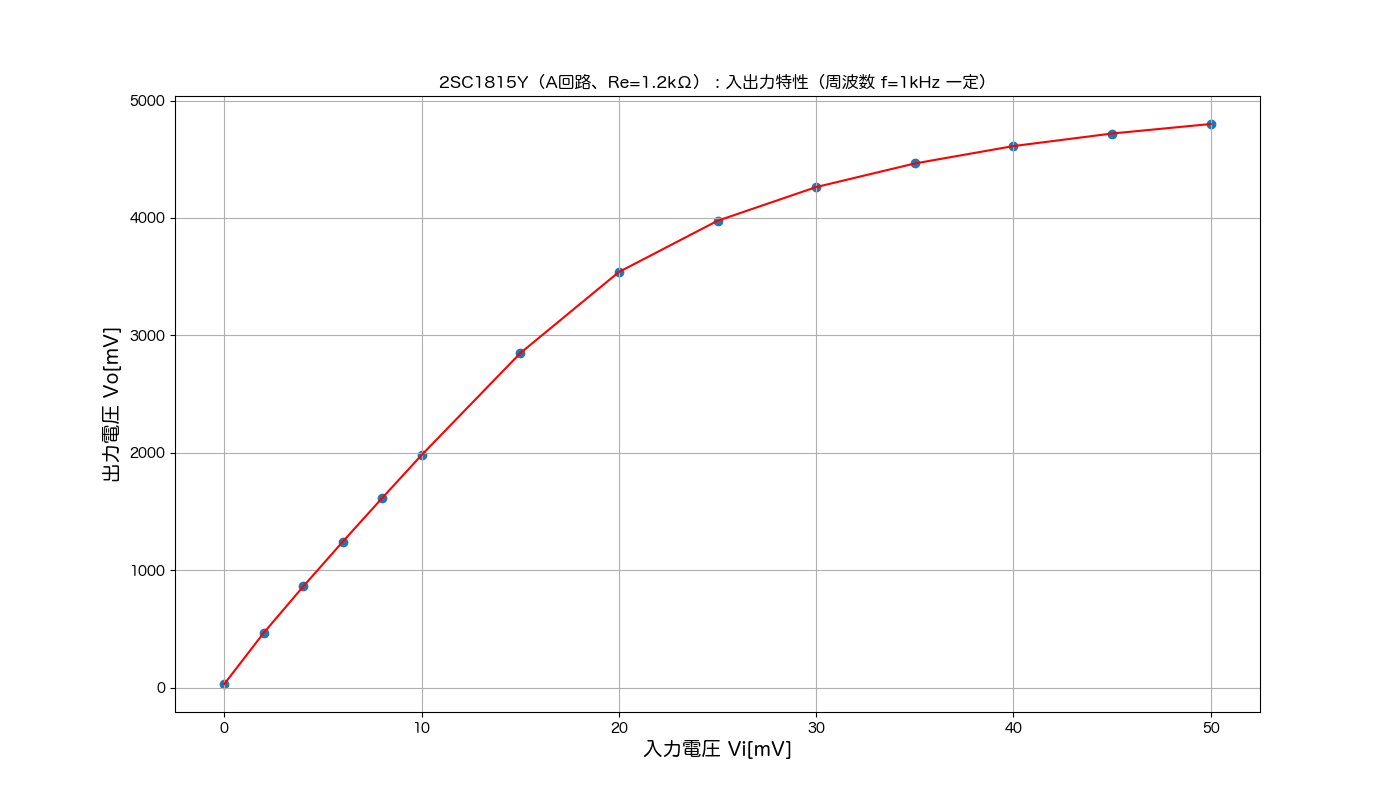
\includegraphics[keepaspectratio, scale=0.65, angle=90]
               {figs/png/iocharM1Y1_2kR.png}
               \caption{教科書モデルでの入出力特性の測定(2SC1815Y, $h_{FE}=174,\;R_E=1.2k\Omega,\;R_B=85.78k\Omega$)}
               \label{fig:9_2_1}
\end{figure}

\newpage

%【入出力特性:2SC1815Y,$h_{FE}=174,\;R_E=1.2k\Omega,\;R_B=85.78k\Omega$】

\begin{spacing}{0.71}
\begin{multicols}{2}
  \begin{figure}[H]
     \centering
      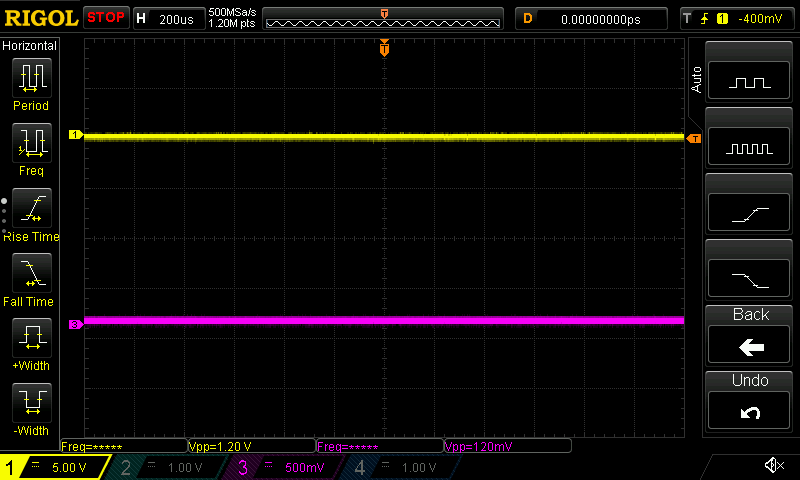
\includegraphics[keepaspectratio, scale=0.28, angle=0]
                  {rigol/figs/IOCharM1Y1_2kR/0mV.png}
                  \caption{$V_i=0\;mV$}
                  \label{fig:ioc0}
  \end{figure}

  \begin{figure}[H]
     \centering
      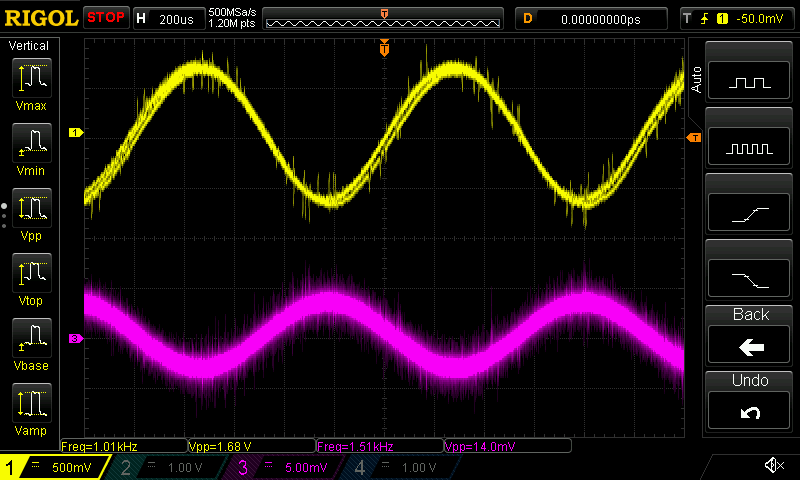
\includegraphics[keepaspectratio, scale=0.28, angle=0]
                {rigol/figs/IOCharM1Y1_2kR/2mV.png}
                \caption{$V_i=2\;mV$}
                \label{fig:ioc2}
  \end{figure}
\end{multicols}

\begin{multicols}{2}
  \begin{figure}[H]
     \centering
      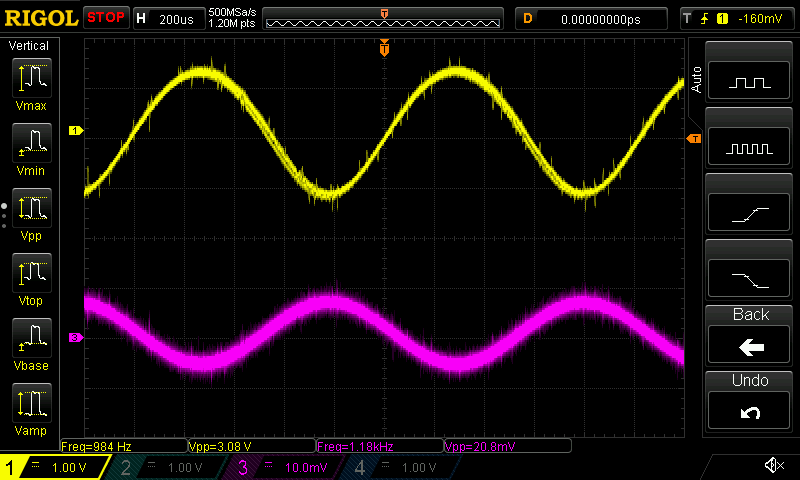
\includegraphics[keepaspectratio, scale=0.28, angle=0]
                  {rigol/figs/IOCharM1Y1_2kR/4mV.png}
                  \caption{$V_i=4\;mV$}
                  \label{fig:ioc4}
  \end{figure}

  \begin{figure}[H]
     \centering
      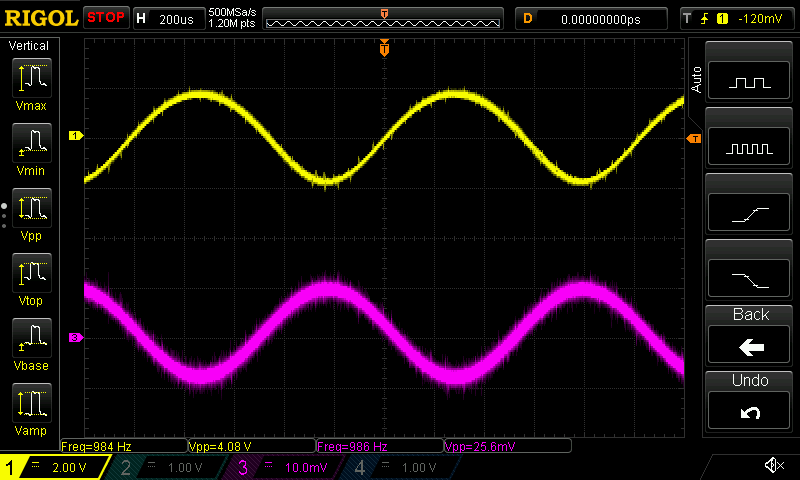
\includegraphics[keepaspectratio, scale=0.28, angle=0]
                {rigol/figs/IOCharM1Y1_2kR/6mV.png}
                \caption{$V_i=6\;mV$}
                \label{fig:ioc6}
  \end{figure}
\end{multicols}

\begin{multicols}{2}
  \begin{figure}[H]
     \centering
      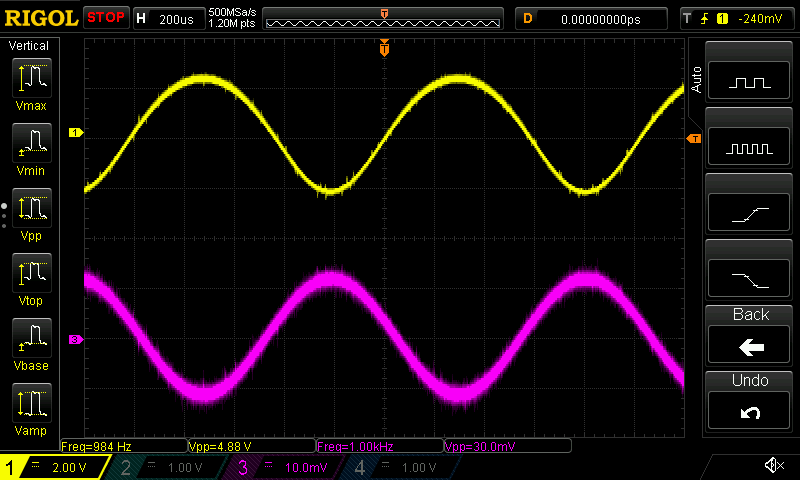
\includegraphics[keepaspectratio, scale=0.28, angle=0]
                  {rigol/figs/IOCharM1Y1_2kR/8mV.png}
                  \caption{$V_i=8\;mV$}
                  \label{fig:ioc8}
  \end{figure}

  \begin{figure}[H]
     \centering
      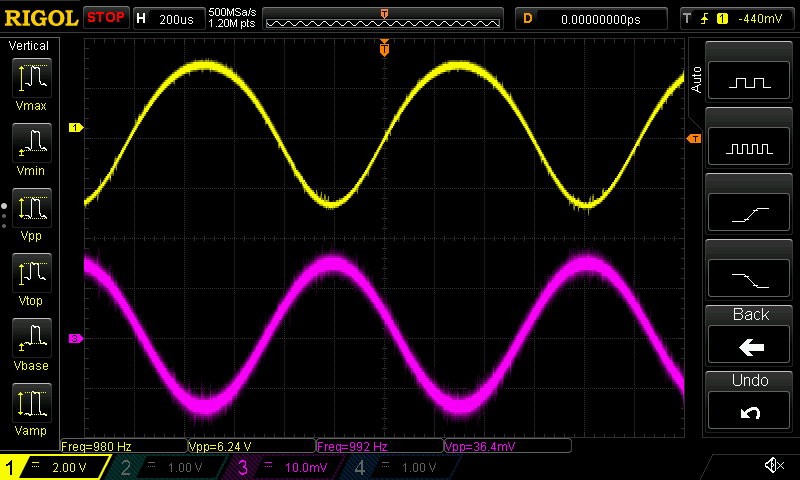
\includegraphics[keepaspectratio, scale=0.28, angle=0]
                {rigol/figs/IOCharM1Y1_2kR/10mV.png}
                \caption{$V_i=10\;mV$}
                \label{fig:ioc10}
  \end{figure}
\end{multicols}

\begin{multicols}{2}
  \begin{figure}[H]
     \centering
      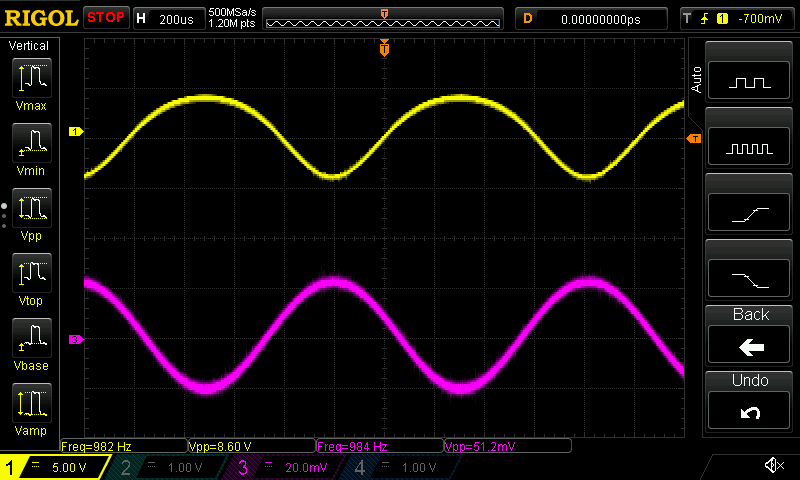
\includegraphics[keepaspectratio, scale=0.28, angle=0]
                  {rigol/figs/IOCharM1Y1_2kR/15mV.png}
                  \caption{$V_i=15\;mV$}
                  \label{fig:ioc15}
  \end{figure}

  \begin{figure}[H]
     \centering
      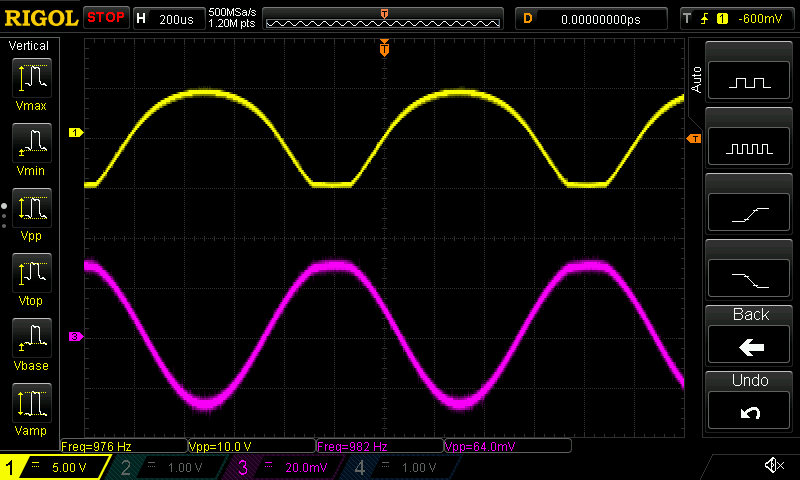
\includegraphics[keepaspectratio, scale=0.28, angle=0]
                {rigol/figs/IOCharM1Y1_2kR/20mV.png}
                \caption{$V_i=20\;mV$}
                \label{fig:ioc20}
  \end{figure}
\end{multicols}

\begin{multicols}{2}
  \begin{figure}[H]
     \centering
      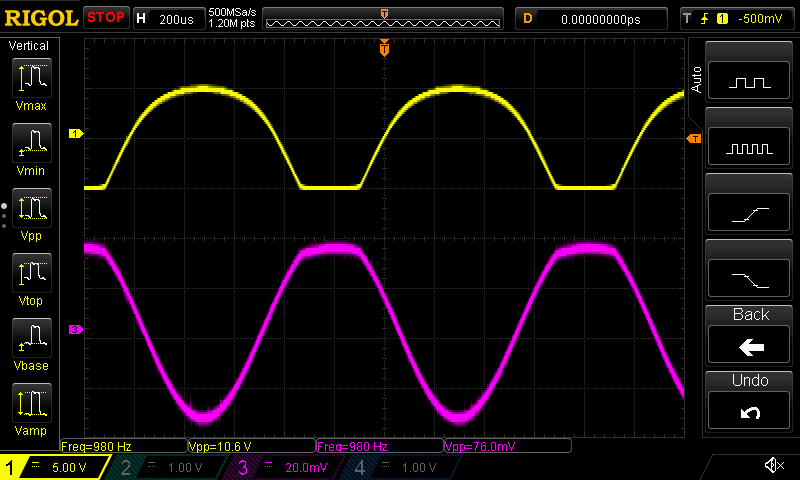
\includegraphics[keepaspectratio, scale=0.28, angle=0]
                  {rigol/figs/IOCharM1Y1_2kR/25mV.png}
                  \caption{$V_i=25\;mV$}
                  \label{fig:ioc25}
  \end{figure}

  \begin{figure}[H]
     \centering
      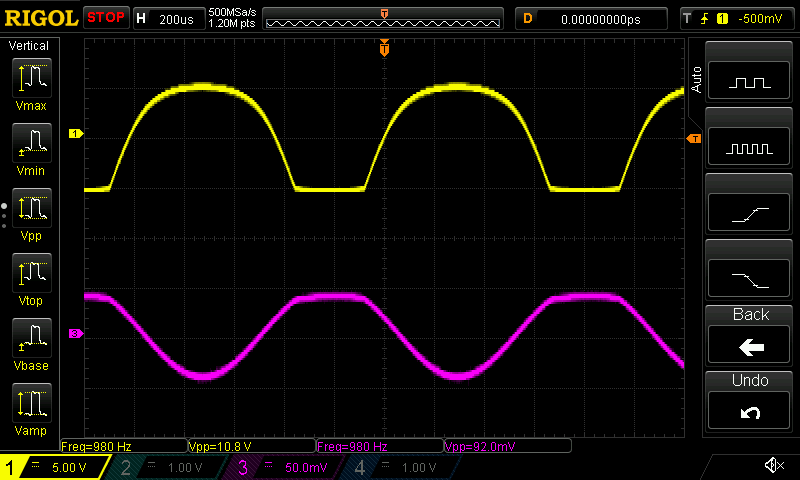
\includegraphics[keepaspectratio, scale=0.28, angle=0]
                {rigol/figs/IOCharM1Y1_2kR/30mV.png}
                \caption{$V_i=30\;mV$}
                \label{fig:ioc30}
  \end{figure}
\end{multicols}

\begin{multicols}{2}
  \begin{figure}[H]
     \centering
      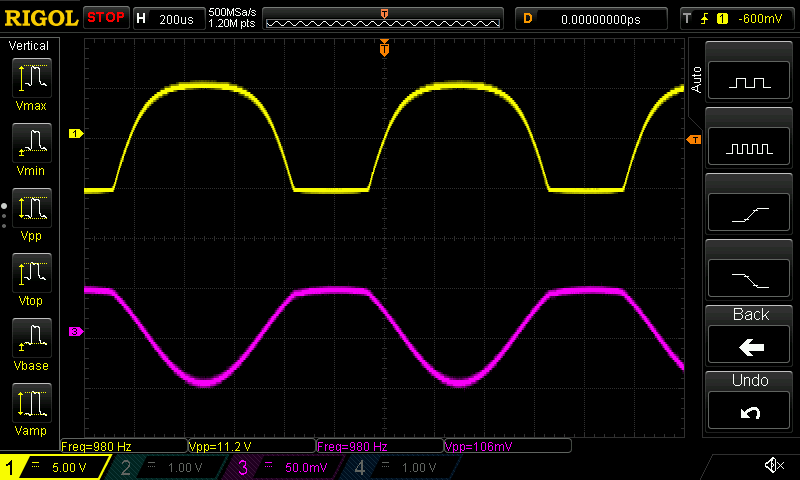
\includegraphics[keepaspectratio, scale=0.28, angle=0]
                  {rigol/figs/IOCharM1Y1_2kR/35mV.png}
                  \caption{$V_i=35\;mV$}
                  \label{fig:ioc35}
  \end{figure}

  \begin{figure}[H]
     \centering
      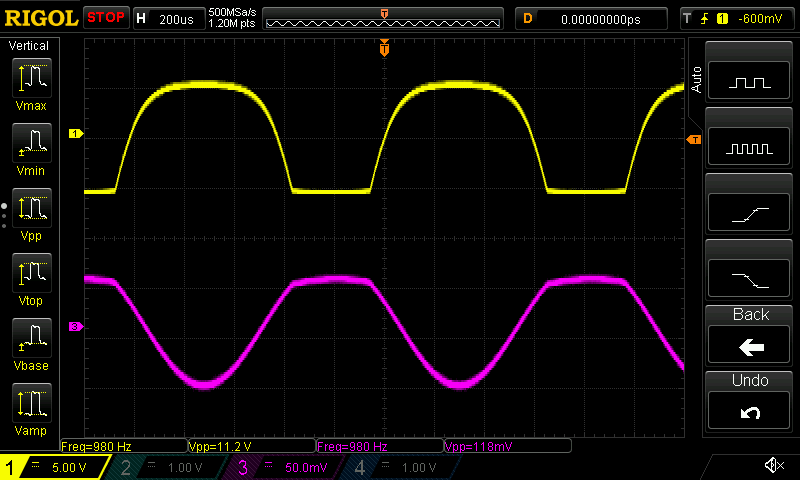
\includegraphics[keepaspectratio, scale=0.28, angle=0]
                {rigol/figs/IOCharM1Y1_2kR/40mV.png}
                \caption{$V_i=40\;mV$}
                \label{fig:ioc40}
  \end{figure}
\end{multicols}

\begin{multicols}{2}
  \begin{figure}[H]
     \centering
      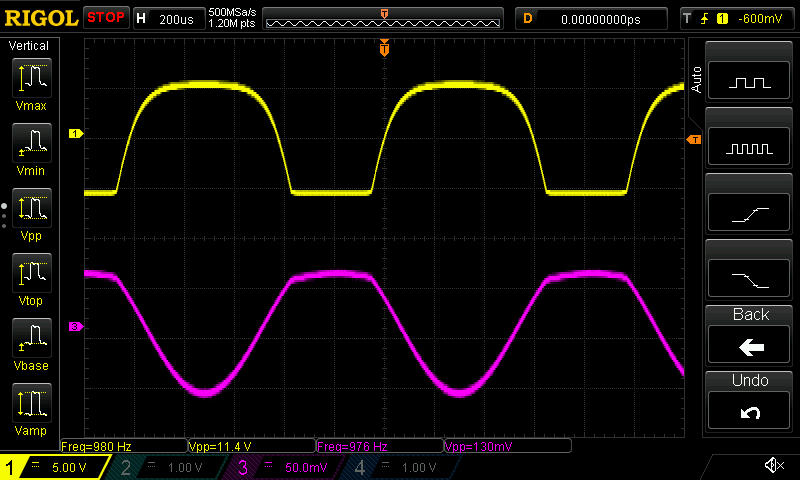
\includegraphics[keepaspectratio, scale=0.28, angle=0]
                  {rigol/figs/IOCharM1Y1_2kR/45mV.png}
                  \caption{$V_i=45\;mV$}
                  \label{fig:ioc45}
  \end{figure}

  \begin{figure}[H]
     \centering
      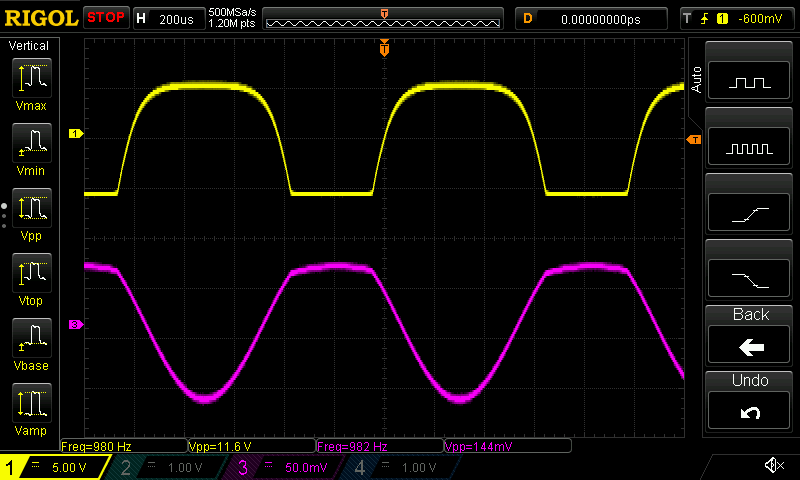
\includegraphics[keepaspectratio, scale=0.28, angle=0]
                {rigol/figs/IOCharM1Y1_2kR/50mV.png}
                \caption{$V_i=50\;mV$}
                \label{fig:ioc50}
  \end{figure}
\end{multicols}
\end{spacing}

\begin{enumerate}
\item[(1)] 入力電圧$V_i=10$[mV] を超えたあたりから波形が潰れ始めている\\
(従って、次の周波数応答の実験では、入力電圧を$5m$Vとして実施している)
\item[(2)] 入力電圧$V_i$と出力電圧$V_o$の波形から、位相が$\pi$[rad] だけずれているのが分かる
\end{enumerate}

\newpage

\begin{figure}[H]
  \centering
   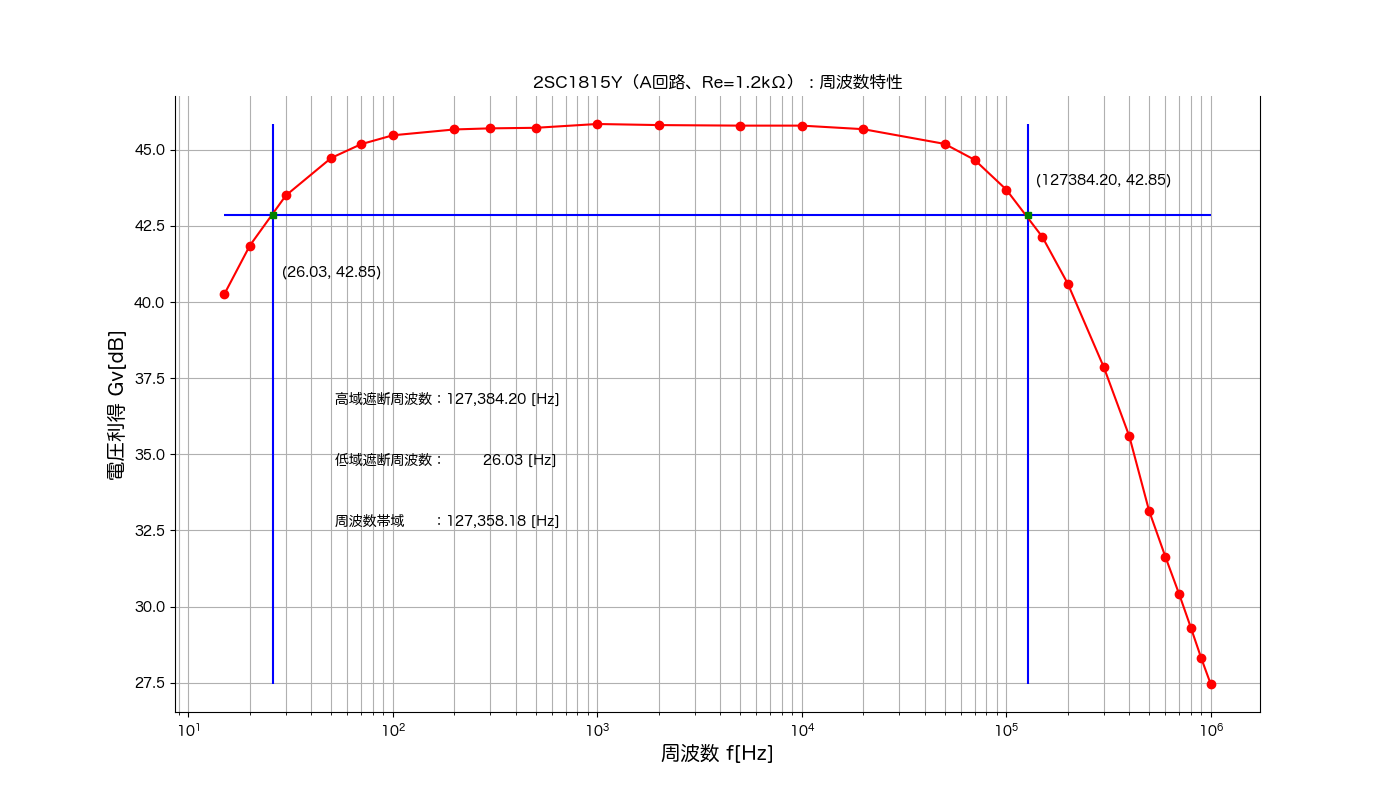
\includegraphics[keepaspectratio, scale=0.65, angle=90]
               {figs/png/freqcharM1Y1_2kR.png}
               \caption{教科書モデルでの周波数特性の測定(2SC1815Y, $h_{FE}=174,\;R_E=1.2k\Omega,\;R_B=85.78k\Omega$)}
               \label{fig:9_2_2}
\end{figure}

\newpage

%【周波数特性:2SC1815Y,$h_{FE}=174,\;R_E=1.2k\Omega,\;R_B=85.78k\Omega$】

\begin{spacing}{0.67}
  \begin{multicols}{2}
    \begin{figure}[H]
       \centering
        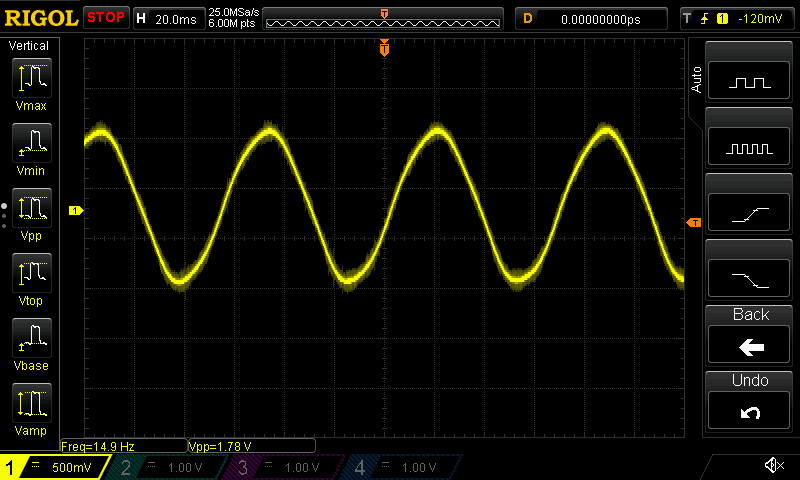
\includegraphics[keepaspectratio, scale=0.28, angle=0]
                    {rigol/figs/FrqCharM1Y1_2kR/15hz.png}
                    \caption{$f=15\;Hz$}
                    \label{fig:frq15}
    \end{figure}
  
    \begin{figure}[H]
       \centering
        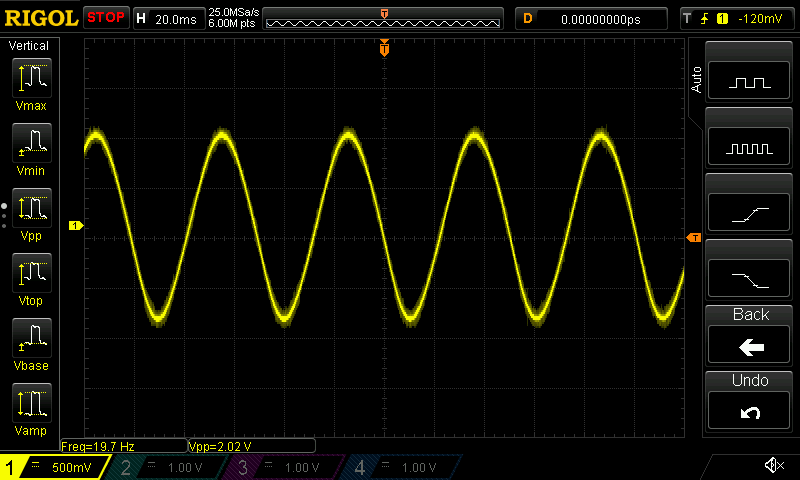
\includegraphics[keepaspectratio, scale=0.28, angle=0]
                  {rigol/figs/FrqCharM1Y1_2kR/20hz.png}
                  \caption{$f=20\;Hz$}
                  \label{fig:frq20}
    \end{figure}
  \end{multicols}

  \begin{multicols}{2}
    \begin{figure}[H]
       \centering
        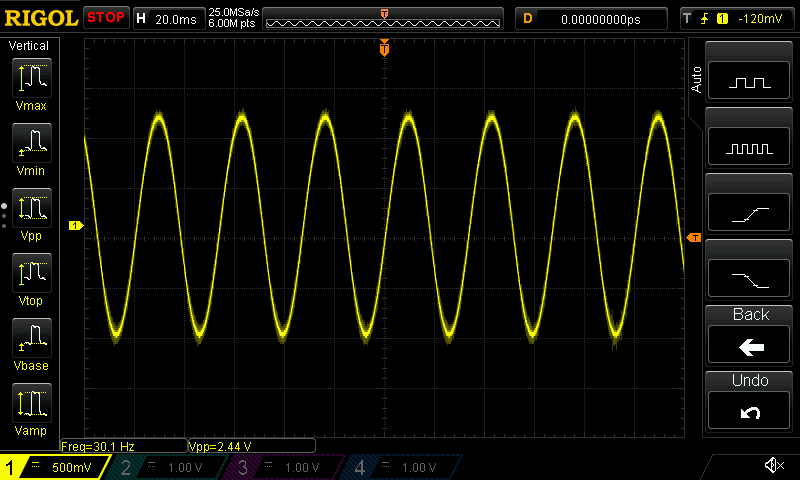
\includegraphics[keepaspectratio, scale=0.28, angle=0]
                    {rigol/figs/FrqCharM1Y1_2kR/30hz.png}
                    \caption{$f=30\;Hz$}
                    \label{fig:frq30}
    \end{figure}
  
    \begin{figure}[H]
       \centering
        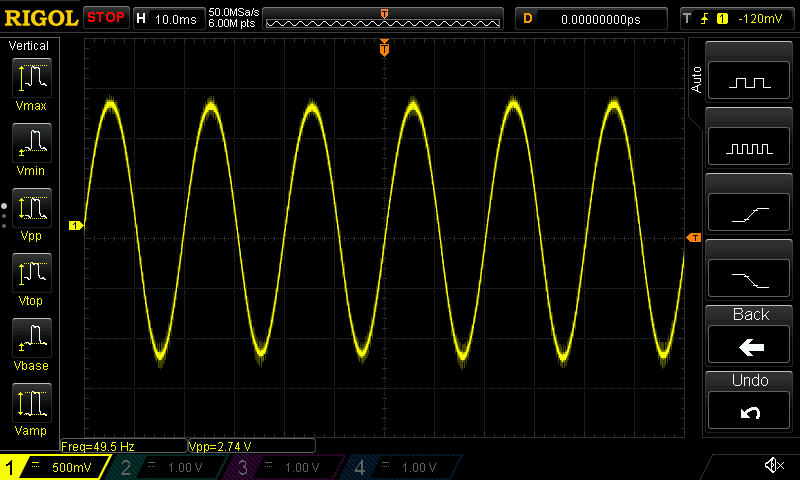
\includegraphics[keepaspectratio, scale=0.28, angle=0]
                  {rigol/figs/FrqCharM1Y1_2kR/50hz.png}
                  \caption{$f=50\;Hz$}
                  \label{fig:frq50}
    \end{figure}
  \end{multicols}

  \begin{multicols}{2}
    \begin{figure}[H]
       \centering
        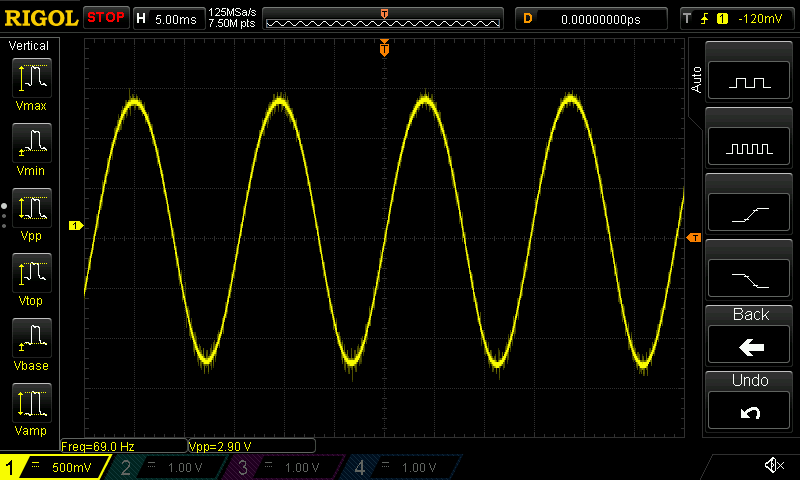
\includegraphics[keepaspectratio, scale=0.28, angle=0]
                    {rigol/figs/FrqCharM1Y1_2kR/70hz.png}
                    \caption{$f=70\;Hz$}
                    \label{fig:frq70}
    \end{figure}
  
    \begin{figure}[H]
       \centering
        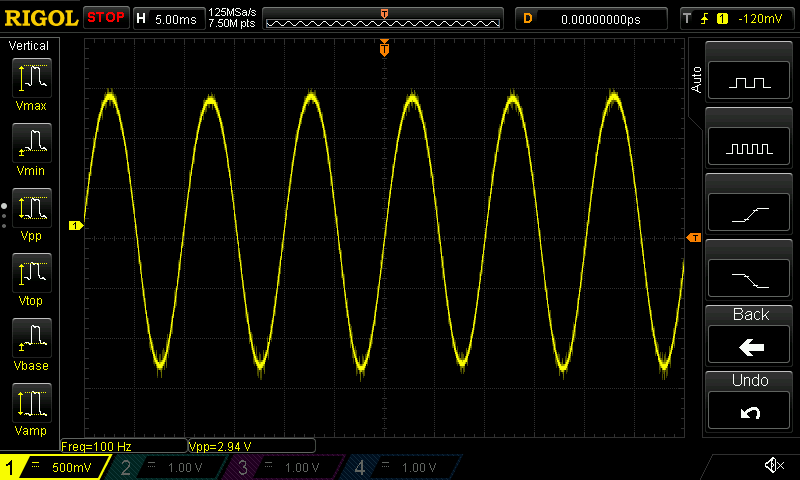
\includegraphics[keepaspectratio, scale=0.28, angle=0]
                  {rigol/figs/FrqCharM1Y1_2kR/100hz.png}
                  \caption{$f=100\;Hz$}
                  \label{fig:frq100}
    \end{figure}
  \end{multicols}

  \begin{multicols}{2}
    \begin{figure}[H]
       \centering
        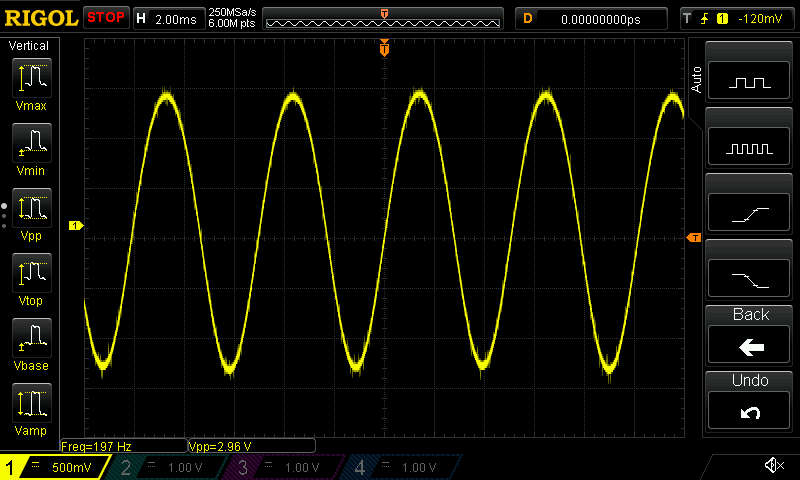
\includegraphics[keepaspectratio, scale=0.28, angle=0]
                    {rigol/figs/FrqCharM1Y1_2kR/200hz.png}
                    \caption{$f=200\;Hz$}
                    \label{fig:frq200}
    \end{figure}
  
    \begin{figure}[H]
       \centering
        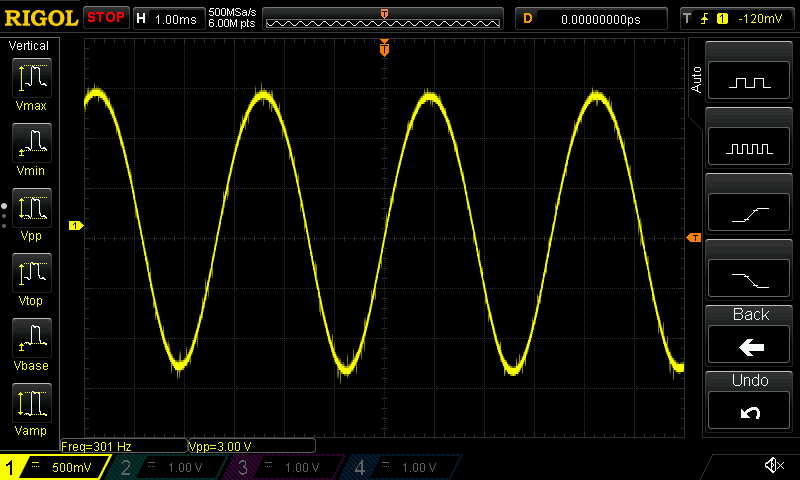
\includegraphics[keepaspectratio, scale=0.28, angle=0]
                  {rigol/figs/FrqCharM1Y1_2kR/300hz.png}
                  \caption{$f=300\;Hz$}
                  \label{fig:frq300}
    \end{figure}
  \end{multicols}

  \begin{multicols}{2}
    \begin{figure}[H]
       \centering
        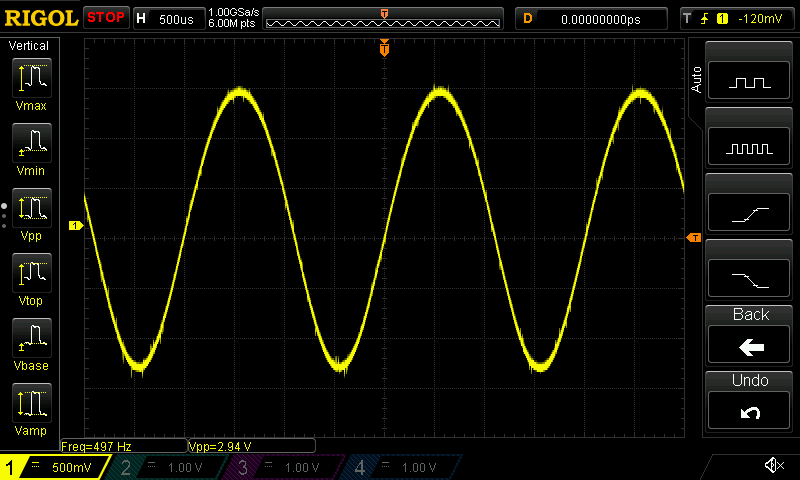
\includegraphics[keepaspectratio, scale=0.28, angle=0]
                    {rigol/figs/FrqCharM1Y1_2kR/500hz.png}
                    \caption{$f=500\;Hz$}
                    \label{fig:frq500}
    \end{figure}
  
    \begin{figure}[H]
       \centering
        \includegraphics[keepaspectratio, scale=0.28, angle=0]
                  {rigol/figs/FrqCharM1Y1_2kR/1khz.png}
                  \caption{$f=1\;kHz$}
                  \label{fig:frq1k}
    \end{figure}
  \end{multicols}

  \begin{multicols}{2}
    \begin{figure}[H]
       \centering
        \includegraphics[keepaspectratio, scale=0.28, angle=0]
                    {rigol/figs/FrqCharM1Y1_2kR/2khz.png}
                    \caption{$f=2\;kHz$}
                    \label{fig:frq2k}
    \end{figure}
  
    \begin{figure}[H]
       \centering
        \includegraphics[keepaspectratio, scale=0.28, angle=0]
                  {rigol/figs/FrqCharM1Y1_2kR/5khz.png}
                  \caption{$f=5\;kHz$}
                  \label{fig:frq5k}
    \end{figure}
  \end{multicols}

  \begin{multicols}{2}
    \begin{figure}[H]
       \centering
        \includegraphics[keepaspectratio, scale=0.28, angle=0]
                    {rigol/figs/FrqCharM1Y1_2kR/10khz.png}
                    \caption{$f=10\;kHz$}
                    \label{fig:frq10k}
    \end{figure}
  
    \begin{figure}[H]
       \centering
        \includegraphics[keepaspectratio, scale=0.28, angle=0]
                  {rigol/figs/FrqCharM1Y1_2kR/20khz.png}
                  \caption{$f=20\;kHz$}
                  \label{fig:frq20k}
    \end{figure}
  \end{multicols}

  \begin{multicols}{2}
    \begin{figure}[H]
       \centering
        \includegraphics[keepaspectratio, scale=0.28, angle=0]
                    {rigol/figs/FrqCharM1Y1_2kR/50khz.png}
                    \caption{$f=50\;kHz$}
                    \label{fig:frq50k}
    \end{figure}
  
    \begin{figure}[H]
       \centering
        \includegraphics[keepaspectratio, scale=0.28, angle=0]
                  {rigol/figs/FrqCharM1Y1_2kR/70khz.png}
                  \caption{$f=70\;kHz$}
                  \label{fig:frq70k}
    \end{figure}
  \end{multicols}

  \begin{multicols}{2}
    \begin{figure}[H]
       \centering
        \includegraphics[keepaspectratio, scale=0.28, angle=0]
                    {rigol/figs/FrqCharM1Y1_2kR/100khz.png}
                    \caption{$f=100\;kHz$}
                    \label{fig:frq100k}
    \end{figure}
  
    \begin{figure}[H]
       \centering
        \includegraphics[keepaspectratio, scale=0.28, angle=0]
                  {rigol/figs/FrqCharM1Y1_2kR/150khz.png}
                  \caption{$f=150\;kHz$}
                  \label{fig:frq150k}
    \end{figure}
  \end{multicols}

  \begin{multicols}{2}
    \begin{figure}[H]
       \centering
        \includegraphics[keepaspectratio, scale=0.28, angle=0]
                    {rigol/figs/FrqCharM1Y1_2kR/200khz.png}
                    \caption{$f=200\;kHz$}
                    \label{fig:frq200k}
    \end{figure}
  
    \begin{figure}[H]
       \centering
        \includegraphics[keepaspectratio, scale=0.28, angle=0]
                  {rigol/figs/FrqCharM1Y1_2kR/300khz.png}
                  \caption{$f=300\;kHz$}
                  \label{fig:frq300k}
    \end{figure}
  \end{multicols}

  \begin{multicols}{2}
    \begin{figure}[H]
       \centering
        \includegraphics[keepaspectratio, scale=0.28, angle=0]
                    {rigol/figs/FrqCharM1Y1_2kR/400khz.png}
                    \caption{$f=400\;kHz$}
                    \label{fig:frq400k}
    \end{figure}
  
    \begin{figure}[H]
       \centering
        \includegraphics[keepaspectratio, scale=0.28, angle=0]
                  {rigol/figs/FrqCharM1Y1_2kR/500khz.png}
                  \caption{$f=500\;kHz$}
                  \label{fig:frq500k}
    \end{figure}
  \end{multicols}

  \begin{multicols}{2}
    \begin{figure}[H]
       \centering
        \includegraphics[keepaspectratio, scale=0.28, angle=0]
                    {rigol/figs/FrqCharM1Y1_2kR/600khz.png}
                    \caption{$f=600\;kHz$}
                    \label{fig:frq600k}
    \end{figure}
  
    \begin{figure}[H]
       \centering
        \includegraphics[keepaspectratio, scale=0.28, angle=0]
                  {rigol/figs/FrqCharM1Y1_2kR/700khz.png}
                  \caption{$f=700\;kHz$}
                  \label{fig:frq700k}
    \end{figure}
  \end{multicols}

  \begin{multicols}{2}
    \begin{figure}[H]
       \centering
        \includegraphics[keepaspectratio, scale=0.28, angle=0]
                    {rigol/figs/FrqCharM1Y1_2kR/800khz.png}
                    \caption{$f=800\;kHz$}
                    \label{fig:frq800k}
    \end{figure}
  
    \begin{figure}[H]
       \centering
        \includegraphics[keepaspectratio, scale=0.28, angle=0]
                  {rigol/figs/FrqCharM1Y1_2kR/1Mhz.png}
                  \caption{$f=1\;MHz$}
                  \label{fig:frq1M}
    \end{figure}
  \end{multicols}
\end{spacing}  

\begin{enumerate}
  \item[(1)] 後半で振幅は少しづつ小さくなっていくのがわかる
  \item[(2)] 全周波数域(15Hz 〜 1MHz)で、波形が潰れることなく、きれいに出力されている\\
(動作点と入力電圧の設定が適切だった)
\end{enumerate}

\newpage

\subsection{代替トランジスタ}

4種類の 2SC1815 があるので、それぞれを使って特性を測定した。
測定に使った回路定数については、
表\ref{table:type}に示す$h_{FE}$と$R_B$の値以外は全て同じ($R_E=1.2k\Omega$など共通)にしている。

$R_B$の値は、4つの実験で共通して$I_C=1\;mA$となる様に半固定抵抗器
\footnote{$R_B$を調節する半固定抵抗器は、
$V_{BE}\fallingdotseq 0.6\;V$周辺のデリケートな領域を調整しなければならないので、
特に多回転半固定抵抗器(高精度25回転)を使用する。}
を使って調整した。

$R_B$を調節することによって、
$R_A$と$R_B$による$V_{CC}$の分圧で$V_B=$($V_{RA}$)が決まり、
それが$I_B$を変化させ、その$h_{FE}$倍である$I_C=1mA$が決定している。
$I_C=1\;mA$が決まれば、その電流による$R_C$での電圧降下が$(V_{CC}-V_E)/2$となるように$R_C$を決めていたのだから、
$V_{CE}\fallingdotseq V_{RC}$を実現できる。\footnote{$V_{CE}$を直接観測しながら、$V_{CE}=(V_{CC}-V_E)/2$となる様に$R_B$を調整する方法も考えられるが、$\cdots$}

表\ref{table:type}から分かる様に、$h_{FE}$の大きいトランジスタほど、
$I_B$が小さくなっている(何れも$I_C=1\;mA$となるために)のが分かる。
($h_{FE}\times I_B$を計算してみると、$938.34\mu A$、$957.44\mu A$、$980.2\mu A$、$954.73\mu A$)

\begin{table}[hbtp]
  \caption{代替トランジスタの実験}
  \label{table:type}
  \centering
  \begin{tabular}{c||l|r||l|r|rrr} \hline
    番号 & 種類 & $h_{FE}$の範囲 & 測定回路で使った値 & $I_B\;[\mu A]$ &$f_L$[Hz] & $f_H$[Hz] & $B$[Hz] \\ \hline \hline
    1 & Orange & 70〜140 & $h_{FE}=117, R_B=83.23k\Omega$ & 8.02 & $27.1$&$193.0k$&$193.0k$ \\
    2 & Yellow & 120〜240 & $h_{FE}=176, R_B=85.83k\Omega$ & 5.44 & $25.4$&$198.6k$&$198.6k$ \\
    3 & GReen & 200〜400 & $h_{FE}=260, R_B=87.42k\Omega$ & 3.77 & $24.7$&$199.5k$&$199.5k$ \\
    4 & BLue & 350〜700 & $h_{FE}=593, R_B=90.78k\Omega$ & 1.61 & $21.7$&$199.8k$&$199.7k$ \\ \hline
  \end{tabular}
\end{table}

実測結果のグラフを重ね合わせてみると、4つのグラフは概ね重なっている。

結論として、この実習においては$I_C=1mA$になる様に$R_B$を調整することによって、
どのトランジスタも代替となり得ることが分かる。実習装置には、
$R_B$の値を表\ref{table:type}の通りの調整範囲に含める様な半固定抵抗器を
用意する(例えば、$R_B$は抵抗器$68k\Omega$と半固定抵抗器$50k\Omega$の直列接続にする)ことと、
コレクタ電流$I_C$を測定できる端子を備える必要がある。

\vfill

\begin{enumerate}
\item $I_C=1\;mA$になる様に$R_B$を調整する手順
\begin{enumerate}
\item[(1)] 実習装置にはトランジスタがセットされた状態であることを確認する
\item[(2)] $I_C$測定端子を短絡しているショートピンを外す
\item[(3)] 露になった$I_C$測定端子に、鰐口クリップを付けたプローブを接続する
\item[(4)] プローブの鰐口クリップ側を回路計(電流計)に接続する
\item[(5)] 実習装置に接続した直流電源装置$E_C(V_{CC}=12V)$のOutputをOnにする
\item[(6)] 回路計(電流計)を読んで、$I_C=1\;mA$となる様に、$R_B$の半固定抵抗器を調整する
\item[(7)] 調整を終えたら、\\①$V_{CC}$をOFFにして、②$I_C$測定用プローブを取り外し、③ショートピンを元に戻す
\end{enumerate}

\vfill

\item $I_C$が$1\;mA$になった時の$R_B$の抵抗値を知るための手順
\begin{enumerate}
\item[(1)] トランジスタを実習装置から取り外す
\item[(2)] 電源装置が実習装置に接続されていないことを確認する\\
(電源装置のOutputがOFFであっても、とにかく実習装置に電源装置を接続しない)
\item[(3)] 回路計で$R_B$を測定する(トランジスタのベース端子と$V_{CC}$のプラス側端子の間で)
\end{enumerate}
\end{enumerate}

\newpage

\begin{spacing}{0.3}
  \begin{multicols}{2}
  \begin{figure}[H]
    %\centering
     \includegraphics[keepaspectratio, scale=0.24, angle=0]
                 {figs/jpg/DSC_0308x.jpg}
                 \caption{自作プローブ}
                 \label{fig:pic3}
  \end{figure}

  \begin{figure}[H]
    %\centering
     \includegraphics[keepaspectratio, scale=0.34, angle=0]
               {figs/jpg/DSC_0311x.jpg}
               \caption{ショートピンを外したところ}
               \label{fig:pic4}
  \end{figure}
  \end{multicols}
\end{spacing}

\begin{spacing}{1}
  %\begin{multicols}{2}
    \begin{figure}[H]
      \centering
       \includegraphics[keepaspectratio, scale=0.32, angle=0]
                 {figs/jpg/DSC_0296x.jpg}
                 \caption{$I_C$を測定して、$I_C=1$mAとなる様に$R_B$の半固定抵抗器を調整する}
                 \label{fig:pic5}
    \end{figure}

    %\begin{figure}[H]
    %\centering
    % \includegraphics[keepaspectratio, scale=0.25, angle=0]
    %             {figs/jpg/DSC_0309x.jpg}
    %             \caption{ショートピンを外している}
    %             \label{fig:pic6}
    %\end{figure}
  %\end{multicols}
\end{spacing}

\newpage

\subsubsection{2SC1815Orange}

\begingroup
\renewcommand{\arraystretch}{1.0}
\begin{table}[H]
  \begin{center}
  \caption{教科書の回路における実測値(回路計による)2SC1815O }\label{tblo}
  \begin{tabular}{|c|l|wr{1.8cm}|l|} \hline
    \multicolumn{1}{|c|}{\textbf{項番}} & \multicolumn{1}{c|}{\textbf{項目}} & \multicolumn{1}{c|}{\textbf{実測値}} & \multicolumn{1}{c|}{\textbf{備考}} \\ \hline
    1 & $R_E$ & $1.200\;k\Omega$ & エミッタ端子とGND端子の間で測定\footnotemark\\
    2 & $R_C$ & $5.571\;k\Omega$ & コレクタ端子と$V_{CC}$の+端子の間で測定\\
    3 & $R_A$ & $15.90\;k\Omega$ & ベース端子とGND端子の間で測定\\
    4 & $R_B$ & $83.23\;k\Omega$ & ベース端子と$V_{CC}$の+端子の間で測定\\
    5 & $V_{CC}$ & $12.30\;V$ & DC12V \\
    6 & $h_{FE}$ & $117$ & 2SC1815-O\\ \hline
    7 & $I_C$ & $1000.0\mu A$ & $I_C=1mA$になるように$R_B$を調整した\\
    8 & $I_B$ & $8.02\mu A$ & \\
    9 & $I_E$ & $578.5\mu A$ & ? \\
    10 & $I_A$ & $115.9\mu A$ & ($20\times I_B=20\times 8.02=160.4\;\mu A$)\\
    11 & $R_B$の電流 & $124.3\mu A$ & $I_A+I_B=115.9+8.02=123.92\;\mu A$ \\
    12 & 全電流 & $1.124mA$ & $I_A+I_B+I_C=115.9+8.02+1000=1.12392\;mA$\\ \hline
    13 & $V_{RC}$ & $5.571\;V$ & 設計時の目標は$V_{RC}\fallingdotseq V_{CE}=(V_{CC}-V_{RE})/2$\\
    14 & $V_{CE}$ & $5.529\;V$ & $V_{RC}\fallingdotseq V_{CE}$で最大値の大きな交流信号を出力できる\\
    15 & $V_{BE}$ & $0.6561\;V$ & シリコンTrの値\\
    16 & $V_{RE}$ & $1.212\;V$ & 設計時の条件は、$V_{CC}$の$10\%=$( 1.23 )V\\
    17 & $V_B=V_{RA}$ & $1.866\;V$ & $V_{BE}+V_{RE}=0.6561+1.212=$( 1.8681 )V \\
    18 & $V_C=V_{RE}+V_{CE}$ & $6.737\;V$ & $V_{CC}-V_{RC}=12.3-5.571=$( 6.729 )V \\ \hline
  \end{tabular}
  \end{center}
\end{table}
\footnotetext{抵抗値の測定ではトランジスタを実習装置から取り外す}
\endgroup

\vspace{-4mm}

\begin{table}[H]
  \begin{center}
  \caption{教科書の回路における実測値(入出力特性:周波数$\;1\;kHz$一定)}
  \begin{tabular}{|l|c|c|c|c|c|c|c|c|c|c|} \hline
    \rowcolor[rgb]{0.9, 0.9, 0.9}
    \multicolumn{1}{|l|}{\textbf{入力電圧 $V_i$[mV]}} & \multicolumn{1}{c|}{\textbf{0}} & \multicolumn{1}{c|}{\textbf{2}} & \multicolumn{1}{c|}{\textbf{4}} & \multicolumn{1}{c|}{\textbf{6}} & \multicolumn{1}{c|}{\textbf{8}} & \multicolumn{1}{c|}{\textbf{10}} & \multicolumn{1}{c|}{\textbf{15}} & \multicolumn{1}{c|}{\textbf{20}} & \multicolumn{1}{c|}{\textbf{25}} & \multicolumn{1}{c|}{\textbf{30}} \\ \hline
    \multicolumn{1}{|l|}{\cellcolor[rgb]{0.9, 0.9, 0.9}\textbf{出力電圧 $V_o$[mV]}} & 38.6 & 471.8 & 851.7 & 1249 & 1635 & 2007 & 2861 & 3557 & 3988 & 4275 \\ \hline \cline{2-11}
    %\rowcolor[rgb]{0.9, 0.9, 0.9} 
    \multicolumn{1}{c|}{} & \multicolumn{1}{c|}{\cellcolor[rgb]{0.9, 0.9, 0.9}\textbf{35}} & \multicolumn{1}{c|}{\cellcolor[rgb]{0.9, 0.9, 0.9}\textbf{40}} & \multicolumn{1}{c|}{\cellcolor[rgb]{0.9, 0.9, 0.9}\textbf{45}} & \multicolumn{1}{c|}{\cellcolor[rgb]{0.9, 0.9, 0.9}\textbf{50}} & \multicolumn{1}{c|}{\cellcolor[rgb]{0.9, 0.9, 0.9}\textbf{}} & \multicolumn{1}{c|}{\cellcolor[rgb]{0.9, 0.9, 0.9}\textbf{}} & \multicolumn{1}{c|}{\cellcolor[rgb]{0.9, 0.9, 0.9}\textbf{}} & \multicolumn{1}{c|}{\cellcolor[rgb]{0.9, 0.9, 0.9}\textbf{}} & \multicolumn{1}{c|}{\cellcolor[rgb]{0.9, 0.9, 0.9}\textbf{}} & \multicolumn{1}{c|}{\cellcolor[rgb]{0.9, 0.9, 0.9}\textbf{}} \\ \cline{2-11}
    \multicolumn{1}{c|}{} & 4477 & 4621 & 4729 & 4808 & & & & & & \\ \cline{2-11} \cline{2-11}
  \end{tabular}
  \end{center}
\end{table}

\vspace{-4mm}

\begin{table}[H]
  \begin{center}
  \caption{教科書の回路における実測値(周波数特性:入力電圧$\;V_i=5\;mV$一定)}\vspace{-4mm}
  \begin{tabular}{|l|c|c|c|c|c|c|c|c|c|c|} \hline
    \rowcolor[rgb]{0.9, 0.9, 0.9}
    \multicolumn{1}{|l|}{\textbf{周波数 f[Hz]}} & \multicolumn{1}{c|}{\textbf{15}} & \multicolumn{1}{c|}{\textbf{20}} & \multicolumn{1}{c|}{\textbf{30}} & \multicolumn{1}{c|}{\textbf{50}} & \multicolumn{1}{c|}{\textbf{70}} & \multicolumn{1}{c|}{\textbf{100}} & \multicolumn{1}{c|}{\textbf{200}} & \multicolumn{1}{c|}{\textbf{300}} & \multicolumn{1}{c|}{\textbf{500}} & \multicolumn{1}{c|}{\textbf{1k}} \\ \hline
    \multicolumn{1}{|l|}{\cellcolor[rgb]{0.9, 0.9, 0.9}\textbf{出力電圧 $V_o$[mV]}} & 500 & 610 & 740 & 862 & 906 & 940 & 965 & 970 & 980 & 980 \\ \hline \cline{2-11}
    %\rowcolor[rgb]{0.9, 0.9, 0.9} 
    \multicolumn{1}{c|}{} & \multicolumn{1}{c|}{\cellcolor[rgb]{0.9, 0.9, 0.9}\textbf{2k}} & \multicolumn{1}{c|}{\cellcolor[rgb]{0.9, 0.9, 0.9}\textbf{5k}} & \multicolumn{1}{c|}{\cellcolor[rgb]{0.9, 0.9, 0.9}\textbf{10k}} & \multicolumn{1}{c|}{\cellcolor[rgb]{0.9, 0.9, 0.9}\textbf{20k}} & \multicolumn{1}{c|}{\cellcolor[rgb]{0.9, 0.9, 0.9}\textbf{50k}} & \multicolumn{1}{c|}{\cellcolor[rgb]{0.9, 0.9, 0.9}\textbf{70k}} & \multicolumn{1}{c|}{\cellcolor[rgb]{0.9, 0.9, 0.9}\textbf{100k}} & \multicolumn{1}{c|}{\cellcolor[rgb]{0.9, 0.9, 0.9}\textbf{150k}} & \multicolumn{1}{c|}{\cellcolor[rgb]{0.9, 0.9, 0.9}\textbf{200k}} & \multicolumn{1}{c|}{\cellcolor[rgb]{0.9, 0.9, 0.9}\textbf{300k}} \\ \cline{2-11}
    \multicolumn{1}{c|}{} & 989 & 979 & 980 & 971 & 945 & 920 & 870 & 780 & 688 & 539 \\ \cline{2-11} \cline{2-11}
    %\rowcolor[rgb]{0.9, 0.9, 0.9} 
    \multicolumn{1}{c|}{} & \multicolumn{1}{c|}{\cellcolor[rgb]{0.9, 0.9, 0.9}\textbf{400k}} & \multicolumn{1}{c|}{\cellcolor[rgb]{0.9, 0.9, 0.9}\textbf{500k}} & \multicolumn{1}{c|}{\cellcolor[rgb]{0.9, 0.9, 0.9}\textbf{600k}} & \multicolumn{1}{c|}{\cellcolor[rgb]{0.9, 0.9, 0.9}\textbf{700k}} & \multicolumn{1}{c|}{\cellcolor[rgb]{0.9, 0.9, 0.9}\textbf{800k}} & \multicolumn{1}{c|}{\cellcolor[rgb]{0.9, 0.9, 0.9}\textbf{900k}} & \multicolumn{1}{c|}{\cellcolor[rgb]{0.9, 0.9, 0.9}\textbf{1M}} & & & \\ \cline{2-11}
    \multicolumn{1}{c|}{} & 439 & 363 & 308 & 241 & 213 & 190 & 172 & & & \\ \cline{2-11}
  \end{tabular}
  \end{center}
\end{table}

\newpage

%\begin{spacing}{0.67}
%  \begin{multicols}{2}
  \begin{figure}[H]
    \centering
     \includegraphics[keepaspectratio, scale=0.48, angle=0]
                 {figs/png/iocharM1O.png}
                 \caption{入出力特性(2SC1815O:$h_{FE}=117,\;R_B=83.23k\Omega$)}
                 \label{fig:iocharM1O}
 \end{figure}

 \begin{figure}[H]
    \centering
     \includegraphics[keepaspectratio, scale=0.48, angle=0]
               {figs/png/freqcharM1O.png}
               \caption{周波数特性(2SC1815O:$h_{FE}=117,\;R_B=83.23k\Omega$)}
               \label{fig:freqcharM1O}
 \end{figure}
%  \end{multicols}
%\end{spacing}

\newpage

\subsubsection{2SC1815Yellow}

\begingroup
\renewcommand{\arraystretch}{1.0}
\begin{table}[H]
  \begin{center}
  \caption{教科書の回路における実測値(回路計による)2SC1815Y }\label{tbly}
  \begin{tabular}{|c|l|wr{1.8cm}|l|} \hline
    \multicolumn{1}{|c|}{\textbf{項番}} & \multicolumn{1}{c|}{\textbf{項目}} & \multicolumn{1}{c|}{\textbf{実測値}} & \multicolumn{1}{c|}{\textbf{備考}} \\ \hline
    1 & $R_E$ & $1.200\;k\Omega$ & エミッタ端子とGND端子の間で測定\\
    2 & $R_C$ & $5.571\;k\Omega$ & コレクタ端子と$V_{CC}$の+端子の間で測定\footnotemark\\
    3 & $R_A$ & $15.90\;k\Omega$ & ベース端子とGND端子の間で測定\\
    4 & $R_B$ & $85.83\;k\Omega$ & ベース端子と$V_{CC}$の+端子の間で測定\\
    5 & $V_{CC}$ & $12.30\;V$ & DC12V \\
    6 & $h_{FE}$ & $176$ & 2SC1815-Y\\ \hline
    7 & $I_C$ & $1000.1\mu A$ & $I_C=1mA$になるように$R_B$を調整した\\
    8 & $I_B$ & $5.44\mu A$ & \\
    9 & $I_E$ & $570.2\mu A$ & ? \\
    10 & $I_A$ & $114.6\mu A$ & ($20\times I_B=20\times 5.44=108.8\;\mu A$)\\
    11 & $R_B$の電流 & $120.3\mu A$ & $I_A+I_B=114.6+5.44=120.04\;\mu A$ \\
    12 & 全電流 & $1.121mA$ & $I_A+I_B+I_C=114.6+5.44+1000.1=1.12014\;mA$\\ \hline
    13 & $V_{RC}$ & $5.584\;V$ & 設計時の目標は$V_{RC}\fallingdotseq V_{CE}=(V_{CC}-V_{RE})/2$\\
    14 & $V_{CE}$ & $5.502\;V$ & $V_{RC}\fallingdotseq V_{CE}$で最大値の大きな交流信号を出力できる\\
    15 & $V_{BE}$ & $0.6372\;V$ & シリコンTrの値\\
    16 & $V_{RE}$ & $1.212\;V$ & 設計時の条件は、$V_{CC}$の$10\%=$( 1.23 )V\\
    17 & $V_B=V_{RA}$ & $1.848\;V$ & $V_{BE}+V_{RE}=0.6372+1.212=$( 1.8492 )V \\
    18 & $V_C=V_{RE}+V_{CE}$ & $6.712\;V$ & $V_{CC}-V_{RC}=12.3-5.584=$( 6.716 )V \\ \hline
  \end{tabular}
  \end{center}
\end{table}
\footnotetext{抵抗値の測定ではトランジスタを実習装置から取り外す}
\endgroup

\vspace{-4mm}

\begin{table}[H]
  \begin{center}
  \caption{教科書の回路における実測値(入出力特性:周波数$\;1\;kHz$一定)}
  \begin{tabular}{|l|c|c|c|c|c|c|c|c|c|c|} \hline
    \rowcolor[rgb]{0.9, 0.9, 0.9}
    \multicolumn{1}{|l|}{\textbf{入力電圧 $V_i$[mV]}} & \multicolumn{1}{c|}{\textbf{0}} & \multicolumn{1}{c|}{\textbf{2}} & \multicolumn{1}{c|}{\textbf{4}} & \multicolumn{1}{c|}{\textbf{6}} & \multicolumn{1}{c|}{\textbf{8}} & \multicolumn{1}{c|}{\textbf{10}} & \multicolumn{1}{c|}{\textbf{15}} & \multicolumn{1}{c|}{\textbf{20}} & \multicolumn{1}{c|}{\textbf{25}} & \multicolumn{1}{c|}{\textbf{30}} \\ \hline
    \multicolumn{1}{|l|}{\cellcolor[rgb]{0.9, 0.9, 0.9}\textbf{出力電圧 $V_o$[mV]}} & 29 & 469.4 & 836.1 & 1238 & 1622 & 1990 & 2857 & 3547 & 3982 & 4272 \\ \hline \cline{2-11}
    %\rowcolor[rgb]{0.9, 0.9, 0.9} 
    \multicolumn{1}{c|}{} & \multicolumn{1}{c|}{\cellcolor[rgb]{0.9, 0.9, 0.9}\textbf{35}} & \multicolumn{1}{c|}{\cellcolor[rgb]{0.9, 0.9, 0.9}\textbf{40}} & \multicolumn{1}{c|}{\cellcolor[rgb]{0.9, 0.9, 0.9}\textbf{45}} & \multicolumn{1}{c|}{\cellcolor[rgb]{0.9, 0.9, 0.9}\textbf{50}} & \multicolumn{1}{c|}{\cellcolor[rgb]{0.9, 0.9, 0.9}\textbf{}} & \multicolumn{1}{c|}{\cellcolor[rgb]{0.9, 0.9, 0.9}\textbf{}} & \multicolumn{1}{c|}{\cellcolor[rgb]{0.9, 0.9, 0.9}\textbf{}} & \multicolumn{1}{c|}{\cellcolor[rgb]{0.9, 0.9, 0.9}\textbf{}} & \multicolumn{1}{c|}{\cellcolor[rgb]{0.9, 0.9, 0.9}\textbf{}} & \multicolumn{1}{c|}{\cellcolor[rgb]{0.9, 0.9, 0.9}\textbf{}} \\ \cline{2-11}
    \multicolumn{1}{c|}{} & 4475 & 4624 & 4732 & 4813 & & & & & & \\ \cline{2-11} \cline{2-11}
  \end{tabular}
  \end{center}
\end{table}

\vspace{-4mm}

\begin{table}[H]
  \begin{center}
  \caption{教科書の回路における実測値(周波数特性:入力電圧$\;V_i=5\;mV$一定)}\vspace{-4mm}
  \begin{tabular}{|l|c|c|c|c|c|c|c|c|c|c|} \hline
    \rowcolor[rgb]{0.9, 0.9, 0.9}
    \multicolumn{1}{|l|}{\textbf{周波数 f[Hz]}} & \multicolumn{1}{c|}{\textbf{15}} & \multicolumn{1}{c|}{\textbf{20}} & \multicolumn{1}{c|}{\textbf{30}} & \multicolumn{1}{c|}{\textbf{50}} & \multicolumn{1}{c|}{\textbf{70}} & \multicolumn{1}{c|}{\textbf{100}} & \multicolumn{1}{c|}{\textbf{200}} & \multicolumn{1}{c|}{\textbf{300}} & \multicolumn{1}{c|}{\textbf{500}} & \multicolumn{1}{c|}{\textbf{1k}} \\ \hline
    \multicolumn{1}{|l|}{\cellcolor[rgb]{0.9, 0.9, 0.9}\textbf{出力電圧 $V_o$[mV]}} & 522 & 622 & 760 & 874 & 910 & 940 & 961 & 962 & 970 & 971 \\ \hline \cline{2-11}
    %\rowcolor[rgb]{0.9, 0.9, 0.9} 
    \multicolumn{1}{c|}{} & \multicolumn{1}{c|}{\cellcolor[rgb]{0.9, 0.9, 0.9}\textbf{2k}} & \multicolumn{1}{c|}{\cellcolor[rgb]{0.9, 0.9, 0.9}\textbf{5k}} & \multicolumn{1}{c|}{\cellcolor[rgb]{0.9, 0.9, 0.9}\textbf{10k}} & \multicolumn{1}{c|}{\cellcolor[rgb]{0.9, 0.9, 0.9}\textbf{20k}} & \multicolumn{1}{c|}{\cellcolor[rgb]{0.9, 0.9, 0.9}\textbf{50k}} & \multicolumn{1}{c|}{\cellcolor[rgb]{0.9, 0.9, 0.9}\textbf{70k}} & \multicolumn{1}{c|}{\cellcolor[rgb]{0.9, 0.9, 0.9}\textbf{100k}} & \multicolumn{1}{c|}{\cellcolor[rgb]{0.9, 0.9, 0.9}\textbf{150k}} & \multicolumn{1}{c|}{\cellcolor[rgb]{0.9, 0.9, 0.9}\textbf{200k}} & \multicolumn{1}{c|}{\cellcolor[rgb]{0.9, 0.9, 0.9}\textbf{300k}} \\ \cline{2-11}
    \multicolumn{1}{c|}{} & 978 & 972 & 970 & 968 & 942 & 920 & 872 & 782 & 690 & 537 \\ \cline{2-11} \cline{2-11}
    %\rowcolor[rgb]{0.9, 0.9, 0.9} 
    \multicolumn{1}{c|}{} & \multicolumn{1}{c|}{\cellcolor[rgb]{0.9, 0.9, 0.9}\textbf{400k}} & \multicolumn{1}{c|}{\cellcolor[rgb]{0.9, 0.9, 0.9}\textbf{500k}} & \multicolumn{1}{c|}{\cellcolor[rgb]{0.9, 0.9, 0.9}\textbf{600k}} & \multicolumn{1}{c|}{\cellcolor[rgb]{0.9, 0.9, 0.9}\textbf{700k}} & \multicolumn{1}{c|}{\cellcolor[rgb]{0.9, 0.9, 0.9}\textbf{800k}} & \multicolumn{1}{c|}{\cellcolor[rgb]{0.9, 0.9, 0.9}\textbf{900k}} & \multicolumn{1}{c|}{\cellcolor[rgb]{0.9, 0.9, 0.9}\textbf{1M}} & & & \\ \cline{2-11}
    \multicolumn{1}{c|}{} & 432 & 360 & 300 & 238 & 209 & 186 & 168 & & & \\ \cline{2-11}
  \end{tabular}
  \end{center}
\end{table}

\newpage

%\begin{spacing}{0.67}
%  \begin{multicols}{2}
  \begin{figure}[H]
    \centering
     \includegraphics[keepaspectratio, scale=0.48, angle=0]
                 {figs/png/iocharM1Y.png}
                 \caption{入出力特性(2SC1815Y:$h_{FE}=176,\;R_B=85.83k\Omega$)}
                 \label{fig:iocharM1Y}
 \end{figure}

 \begin{figure}[H]
    \centering
     \includegraphics[keepaspectratio, scale=0.48, angle=0]
               {figs/png/freqcharM1Y.png}
               \caption{周波数特性(2SC1815Y:$h_{FE}=176,\;R_B=85.83k\Omega$)}
               \label{fig:freqcharM1Y}
 \end{figure}
%  \end{multicols}
%\end{spacing}

\newpage

\subsubsection{2SC1815GReen}

\begingroup
\renewcommand{\arraystretch}{1.0}
\begin{table}[H]
  \begin{center}
  \caption{教科書の回路における実測値(回路計による)2SC1815GR }\label{tblg}
  \begin{tabular}{|c|l|wr{1.8cm}|l|} \hline
    \multicolumn{1}{|c|}{\textbf{項番}} & \multicolumn{1}{c|}{\textbf{項目}} & \multicolumn{1}{c|}{\textbf{実測値}} & \multicolumn{1}{c|}{\textbf{備考}} \\ \hline
    1 & $R_E$ & $1.200\;k\Omega$ & エミッタ端子とGND端子の間で測定\footnotemark\\
    2 & $R_C$ & $5.571\;k\Omega$ & コレクタ端子と$V_{CC}$の+端子の間で測定\\
    3 & $R_A$ & $15.90\;k\Omega$ & ベース端子とGND端子の間で測定\\
    4 & $R_B$ & $87.42\;k\Omega$ & ベース端子と$V_{CC}$の+端子の間で測定\\
    5 & $V_{CC}$ & $12.30\;V$ & DC12V \\
    6 & $h_{FE}$ & $260$ & 2SC1815-GR\\ \hline
    7 & $I_C$ & $1000.1\mu A$ & $I_C=1mA$になるように$R_B$を調整した\\
    8 & $I_B$ & $3.77\mu A$ & \\
    9 & $I_E$ & $994\mu A$ & \\
    10 & $I_A$ & $115\mu A$ & ($20\times I_B=20\times 3.77=75.4\;\mu A$)\\
    11 & $R_B$の電流 & $119\mu A$ & $I_A+I_B=115+3.77=118.77\;\mu A$ \\
    12 & 全電流 & $1.118mA$ & $I_A+I_B+I_C=114.6+5.44+1000.1=1.11877\;mA$\\ \hline
    13 & $V_{RC}$ & $5.581\;V$ & 設計時の目標は$V_{RC}\fallingdotseq V_{CE}=(V_{CC}-V_{RE})/2$\\
    14 & $V_{CE}$ & $5.504\;V$ & $V_{RC}\fallingdotseq V_{CE}$で最大値の大きな交流信号を出力できる\\
    15 & $V_{BE}$ & $0.6327\;V$ & シリコンTrの値\\
    16 & $V_{RE}$ & $1.210\;V$ & 設計時の条件は、$V_{CC}$の$10\%=$( 1.23 )V\\
    17 & $V_B=V_{RA}$ & $1.841\;V$ & $V_{BE}+V_{RE}=0.6327+1.21=$( 1.8427 )V \\
    18 & $V_C=V_{RE}+V_{CE}$ & $6.711\;V$ & $V_{CC}-V_{RC}=12.3-5.581=$( 6.719 )V \\ \hline
  \end{tabular}
  \end{center}
\end{table}
\footnotetext{抵抗値の測定ではトランジスタを実習装置から取り外す}
\endgroup

\vspace{-4mm}

\begin{table}[H]
  \begin{center}
  \caption{教科書の回路における実測値(入出力特性:周波数$\;1\;kHz$一定)}
  \begin{tabular}{|l|c|c|c|c|c|c|c|c|c|c|} \hline
    \rowcolor[rgb]{0.9, 0.9, 0.9}
    \multicolumn{1}{|l|}{\textbf{入力電圧 $V_i$[mV]}} & \multicolumn{1}{c|}{\textbf{0}} & \multicolumn{1}{c|}{\textbf{2}} & \multicolumn{1}{c|}{\textbf{4}} & \multicolumn{1}{c|}{\textbf{6}} & \multicolumn{1}{c|}{\textbf{8}} & \multicolumn{1}{c|}{\textbf{10}} & \multicolumn{1}{c|}{\textbf{15}} & \multicolumn{1}{c|}{\textbf{20}} & \multicolumn{1}{c|}{\textbf{25}} & \multicolumn{1}{c|}{\textbf{30}} \\ \hline
    \multicolumn{1}{|l|}{\cellcolor[rgb]{0.9, 0.9, 0.9}\textbf{出力電圧 $V_o$[mV]}} & 29.2 & 482.1 & 852.1 & 1251 & 1643 & 2007 & 2888 & 3573 & 3999 & 4285 \\ \hline \cline{2-11}
    %\rowcolor[rgb]{0.9, 0.9, 0.9} 
    \multicolumn{1}{c|}{} & \multicolumn{1}{c|}{\cellcolor[rgb]{0.9, 0.9, 0.9}\textbf{35}} & \multicolumn{1}{c|}{\cellcolor[rgb]{0.9, 0.9, 0.9}\textbf{40}} & \multicolumn{1}{c|}{\cellcolor[rgb]{0.9, 0.9, 0.9}\textbf{45}} & \multicolumn{1}{c|}{\cellcolor[rgb]{0.9, 0.9, 0.9}\textbf{50}} & \multicolumn{1}{c|}{\cellcolor[rgb]{0.9, 0.9, 0.9}\textbf{}} & \multicolumn{1}{c|}{\cellcolor[rgb]{0.9, 0.9, 0.9}\textbf{}} & \multicolumn{1}{c|}{\cellcolor[rgb]{0.9, 0.9, 0.9}\textbf{}} & \multicolumn{1}{c|}{\cellcolor[rgb]{0.9, 0.9, 0.9}\textbf{}} & \multicolumn{1}{c|}{\cellcolor[rgb]{0.9, 0.9, 0.9}\textbf{}} & \multicolumn{1}{c|}{\cellcolor[rgb]{0.9, 0.9, 0.9}\textbf{}} \\ \cline{2-11}
    \multicolumn{1}{c|}{} & 4490 & 4636 & 4746 & 4827 & & & & & & \\ \cline{2-11} \cline{2-11}
  \end{tabular}
  \end{center}
\end{table}

\vspace{-4mm}

\begin{table}[H]
  \begin{center}
  \caption{教科書の回路における実測値(周波数特性:入力電圧$\;V_i=5\;mV$一定)}\vspace{-4mm}
  \begin{tabular}{|l|c|c|c|c|c|c|c|c|c|c|} \hline
    \rowcolor[rgb]{0.9, 0.9, 0.9}
    \multicolumn{1}{|l|}{\textbf{周波数 f[Hz]}} & \multicolumn{1}{c|}{\textbf{15}} & \multicolumn{1}{c|}{\textbf{20}} & \multicolumn{1}{c|}{\textbf{30}} & \multicolumn{1}{c|}{\textbf{50}} & \multicolumn{1}{c|}{\textbf{70}} & \multicolumn{1}{c|}{\textbf{100}} & \multicolumn{1}{c|}{\textbf{200}} & \multicolumn{1}{c|}{\textbf{300}} & \multicolumn{1}{c|}{\textbf{500}} & \multicolumn{1}{c|}{\textbf{1k}} \\ \hline
    \multicolumn{1}{|l|}{\cellcolor[rgb]{0.9, 0.9, 0.9}\textbf{出力電圧 $V_o$[mV]}} & 540 & 640 & 778 & 881 & 925 & 960 & 980 & 985 & 989 & 989 \\ \hline \cline{2-11}
    %\rowcolor[rgb]{0.9, 0.9, 0.9} 
    \multicolumn{1}{c|}{} & \multicolumn{1}{c|}{\cellcolor[rgb]{0.9, 0.9, 0.9}\textbf{2k}} & \multicolumn{1}{c|}{\cellcolor[rgb]{0.9, 0.9, 0.9}\textbf{5k}} & \multicolumn{1}{c|}{\cellcolor[rgb]{0.9, 0.9, 0.9}\textbf{10k}} & \multicolumn{1}{c|}{\cellcolor[rgb]{0.9, 0.9, 0.9}\textbf{20k}} & \multicolumn{1}{c|}{\cellcolor[rgb]{0.9, 0.9, 0.9}\textbf{50k}} & \multicolumn{1}{c|}{\cellcolor[rgb]{0.9, 0.9, 0.9}\textbf{70k}} & \multicolumn{1}{c|}{\cellcolor[rgb]{0.9, 0.9, 0.9}\textbf{100k}} & \multicolumn{1}{c|}{\cellcolor[rgb]{0.9, 0.9, 0.9}\textbf{150k}} & \multicolumn{1}{c|}{\cellcolor[rgb]{0.9, 0.9, 0.9}\textbf{200k}} & \multicolumn{1}{c|}{\cellcolor[rgb]{0.9, 0.9, 0.9}\textbf{300k}} \\ \cline{2-11}
    \multicolumn{1}{c|}{} & 990 & 990 & 982 & 972 & 959 & 940 & 885 & 800 & 700 & 541 \\ \cline{2-11} \cline{2-11}
    %\rowcolor[rgb]{0.9, 0.9, 0.9} 
    \multicolumn{1}{c|}{} & \multicolumn{1}{c|}{\cellcolor[rgb]{0.9, 0.9, 0.9}\textbf{400k}} & \multicolumn{1}{c|}{\cellcolor[rgb]{0.9, 0.9, 0.9}\textbf{500k}} & \multicolumn{1}{c|}{\cellcolor[rgb]{0.9, 0.9, 0.9}\textbf{600k}} & \multicolumn{1}{c|}{\cellcolor[rgb]{0.9, 0.9, 0.9}\textbf{700k}} & \multicolumn{1}{c|}{\cellcolor[rgb]{0.9, 0.9, 0.9}\textbf{800k}} & \multicolumn{1}{c|}{\cellcolor[rgb]{0.9, 0.9, 0.9}\textbf{900k}} & \multicolumn{1}{c|}{\cellcolor[rgb]{0.9, 0.9, 0.9}\textbf{1M}} & & & \\ \cline{2-11}
    \multicolumn{1}{c|}{} & 440 & 362 & 308 & 270 & 238 & 189 & 172 & & & \\ \cline{2-11}
  \end{tabular}
  \end{center}
\end{table}

\newpage

%\begin{spacing}{0.67}
%  \begin{multicols}{2}
  \begin{figure}[H]
    \centering
     \includegraphics[keepaspectratio, scale=0.48, angle=0]
                 {figs/png/iocharM1G.png}
                 \caption{入出力特性(2SC1815GR:$h_{FE}=260,\;R_B=87.42k\Omega$)}
                 \label{fig:iocharM1G}
 \end{figure}

 \begin{figure}[H]
    \centering
     \includegraphics[keepaspectratio, scale=0.48, angle=0]
               {figs/png/freqcharM1G.png}
               \caption{周波数特性(2SC1815GR:$h_{FE}=260,\;R_B=87.42k\Omega$)}
               \label{fig:freqcharM1G}
 \end{figure}
%  \end{multicols}
%\end{spacing}

\newpage

\subsubsection{2SC1815BLue}

\begingroup
\renewcommand{\arraystretch}{1.0}
\begin{table}[H]
  \begin{center}
  \caption{教科書の回路における実測値(回路計による)2SC1815BL }\label{tblb}
  \begin{tabular}{|c|l|wr{1.8cm}|l|} \hline
    \multicolumn{1}{|c|}{\textbf{項番}} & \multicolumn{1}{c|}{\textbf{項目}} & \multicolumn{1}{c|}{\textbf{実測値}} & \multicolumn{1}{c|}{\textbf{備考}} \\ \hline
    1 & $R_E$ & $1.200\;k\Omega$ & エミッタ端子とGND端子の間で測定\\
    2 & $R_C$ & $5.571\;k\Omega$ & コレクタ端子と$V_{CC}$の+端子の間で測定\\
    3 & $R_A$ & $15.90\;k\Omega$ & ベース端子とGND端子の間で測定\\
    4 & $R_B$ & $90.78\;k\Omega$ & ベース端子と$V_{CC}$の+端子の間で測定\footnotemark\\
    5 & $V_{CC}$ & $12.30\;V$ & DC12V \\
    6 & $h_{FE}$ & $593$ & 2SC1815-BL\\ \hline
    7 & $I_C$ & $1000\mu A$ & $I_C=1mA$になるように$R_B$を調整した\\
    8 & $I_B$ & $1.61\mu A$ & \\
    9 & $I_E$ & $558.9\mu A$ & ? \\
    10 & $I_A$ & $113.0\mu A$ & ($20\times I_B=20\times 1.61=32.2\;\mu A$)\\
    11 & $R_B$の電流 & $114.7\mu A$ & $I_A+I_B=113+1.61=114.6\;\mu A$ \\
    12 & 全電流 & $1.114mA$ & $I_A+I_B+I_C=114.6+5.44+1000.1=1.11461\;mA$\\ \hline
    13 & $V_{RC}$ & $5.569\;V$ & 設計時の目標は$V_{RC}\fallingdotseq V_{CE}=(V_{CC}-V_{RE})/2$\\
    14 & $V_{CE}$ & $5.534\;V$ & $V_{RC}\fallingdotseq V_{CE}$で最大値の大きな交流信号を出力できる\\
    15 & $V_{BE}$ & $0.6097\;V$ & シリコンTrの値\\
    16 & $V_{RE}$ & $1.205\;V$ & 設計時の条件は、$V_{CC}$の$10\%=$( 1.23 )V\\
    17 & $V_B=V_{RA}$ & $1.812\;V$ & $V_{BE}+V_{RE}=0.6097+1.205=$( 1.8147 )V \\
    18 & $V_C=V_{RE}+V_{CE}$ & $6.734\;V$ & $V_{CC}-V_{RC}=12.3-5.569=$( 6.731 )V \\ \hline
  \end{tabular}
  \end{center}
\end{table}
\footnotetext{抵抗値の測定ではトランジスタを実習装置から取り外す}
\endgroup

\vspace{-4mm}

\begin{table}[H]
  \begin{center}
  \caption{教科書の回路における実測値(入出力特性:周波数$\;1\;kHz$一定)}
  \begin{tabular}{|l|c|c|c|c|c|c|c|c|c|c|} \hline
    \rowcolor[rgb]{0.9, 0.9, 0.9}
    \multicolumn{1}{|l|}{\textbf{入力電圧 $V_i$[mV]}} & \multicolumn{1}{c|}{\textbf{0}} & \multicolumn{1}{c|}{\textbf{2}} & \multicolumn{1}{c|}{\textbf{4}} & \multicolumn{1}{c|}{\textbf{6}} & \multicolumn{1}{c|}{\textbf{8}} & \multicolumn{1}{c|}{\textbf{10}} & \multicolumn{1}{c|}{\textbf{15}} & \multicolumn{1}{c|}{\textbf{20}} & \multicolumn{1}{c|}{\textbf{25}} & \multicolumn{1}{c|}{\textbf{30}} \\ \hline
    \multicolumn{1}{|l|}{\cellcolor[rgb]{0.9, 0.9, 0.9}\textbf{出力電圧 $V_o$[mV]}} & 36.0 & 459.1 & 837.2 & 1215 & 1594 & 1950 & 2797 & 3501 & 3941 & 4238 \\ \hline \cline{2-11}
    %\rowcolor[rgb]{0.9, 0.9, 0.9} 
    \multicolumn{1}{c|}{} & \multicolumn{1}{c|}{\cellcolor[rgb]{0.9, 0.9, 0.9}\textbf{35}} & \multicolumn{1}{c|}{\cellcolor[rgb]{0.9, 0.9, 0.9}\textbf{40}} & \multicolumn{1}{c|}{\cellcolor[rgb]{0.9, 0.9, 0.9}\textbf{45}} & \multicolumn{1}{c|}{\cellcolor[rgb]{0.9, 0.9, 0.9}\textbf{50}} & \multicolumn{1}{c|}{\cellcolor[rgb]{0.9, 0.9, 0.9}\textbf{}} & \multicolumn{1}{c|}{\cellcolor[rgb]{0.9, 0.9, 0.9}\textbf{}} & \multicolumn{1}{c|}{\cellcolor[rgb]{0.9, 0.9, 0.9}\textbf{}} & \multicolumn{1}{c|}{\cellcolor[rgb]{0.9, 0.9, 0.9}\textbf{}} & \multicolumn{1}{c|}{\cellcolor[rgb]{0.9, 0.9, 0.9}\textbf{}} & \multicolumn{1}{c|}{\cellcolor[rgb]{0.9, 0.9, 0.9}\textbf{}} \\ \cline{2-11}
    \multicolumn{1}{c|}{} & 4452 & 4614 & 4727 & 4816 & & & & & & \\ \cline{2-11} \cline{2-11}
  \end{tabular}
  \end{center}
\end{table}

\vspace{-4mm}

\begin{table}[H]
  \begin{center}
  \caption{教科書の回路における実測値(周波数特性:入力電圧$\;V_i=5\;mV$一定)}\vspace{-4mm}
  \begin{tabular}{|l|c|c|c|c|c|c|c|c|c|c|} \hline
    \rowcolor[rgb]{0.9, 0.9, 0.9}
    \multicolumn{1}{|l|}{\textbf{周波数 f[Hz]}} & \multicolumn{1}{c|}{\textbf{15}} & \multicolumn{1}{c|}{\textbf{20}} & \multicolumn{1}{c|}{\textbf{30}} & \multicolumn{1}{c|}{\textbf{50}} & \multicolumn{1}{c|}{\textbf{70}} & \multicolumn{1}{c|}{\textbf{100}} & \multicolumn{1}{c|}{\textbf{200}} & \multicolumn{1}{c|}{\textbf{300}} & \multicolumn{1}{c|}{\textbf{500}} & \multicolumn{1}{c|}{\textbf{1k}} \\ \hline
    \multicolumn{1}{|l|}{\cellcolor[rgb]{0.9, 0.9, 0.9}\textbf{出力電圧 $V_o$[mV]}} & 554 & 655 & 781 & 879 & 905 & 922 & 943 & 950 & 951 & 952 \\ \hline \cline{2-11}
    %\rowcolor[rgb]{0.9, 0.9, 0.9} 
    \multicolumn{1}{c|}{} & \multicolumn{1}{c|}{\cellcolor[rgb]{0.9, 0.9, 0.9}\textbf{2k}} & \multicolumn{1}{c|}{\cellcolor[rgb]{0.9, 0.9, 0.9}\textbf{5k}} & \multicolumn{1}{c|}{\cellcolor[rgb]{0.9, 0.9, 0.9}\textbf{10k}} & \multicolumn{1}{c|}{\cellcolor[rgb]{0.9, 0.9, 0.9}\textbf{20k}} & \multicolumn{1}{c|}{\cellcolor[rgb]{0.9, 0.9, 0.9}\textbf{50k}} & \multicolumn{1}{c|}{\cellcolor[rgb]{0.9, 0.9, 0.9}\textbf{70k}} & \multicolumn{1}{c|}{\cellcolor[rgb]{0.9, 0.9, 0.9}\textbf{100k}} & \multicolumn{1}{c|}{\cellcolor[rgb]{0.9, 0.9, 0.9}\textbf{150k}} & \multicolumn{1}{c|}{\cellcolor[rgb]{0.9, 0.9, 0.9}\textbf{200k}} & \multicolumn{1}{c|}{\cellcolor[rgb]{0.9, 0.9, 0.9}\textbf{300k}} \\ \cline{2-11}
    \multicolumn{1}{c|}{} & 954 & 953 & 945 & 950 & 929 & 898 & 849 & 762 & 675 & 528 \\ \cline{2-11} \cline{2-11}
    %\rowcolor[rgb]{0.9, 0.9, 0.9} 
    \multicolumn{1}{c|}{} & \multicolumn{1}{c|}{\cellcolor[rgb]{0.9, 0.9, 0.9}\textbf{400k}} & \multicolumn{1}{c|}{\cellcolor[rgb]{0.9, 0.9, 0.9}\textbf{500k}} & \multicolumn{1}{c|}{\cellcolor[rgb]{0.9, 0.9, 0.9}\textbf{600k}} & \multicolumn{1}{c|}{\cellcolor[rgb]{0.9, 0.9, 0.9}\textbf{700k}} & \multicolumn{1}{c|}{\cellcolor[rgb]{0.9, 0.9, 0.9}\textbf{800k}} & \multicolumn{1}{c|}{\cellcolor[rgb]{0.9, 0.9, 0.9}\textbf{900k}} & \multicolumn{1}{c|}{\cellcolor[rgb]{0.9, 0.9, 0.9}\textbf{1M}} & & & \\ \cline{2-11}
    \multicolumn{1}{c|}{} & 428 & 357 & 276 & 234 & 209 & 185 & 167 & & & \\ \cline{2-11}
  \end{tabular}
  \end{center}
\end{table}

\newpage

%\begin{spacing}{0.67}
%  \begin{multicols}{2}
  \begin{figure}[H]
    \centering
     \includegraphics[keepaspectratio, scale=0.48, angle=0]
                 {figs/png/iocharM1B.png}
                 \caption{入出力特性(2SC1815BL:$h_{FE}=593,\;R_B=90.78k\Omega$)}
                 \label{fig:iocharM1B}
 \end{figure}

 \begin{figure}[H]
    \centering
     \includegraphics[keepaspectratio, scale=0.48, angle=0]
               {figs/png/freqcharM1B.png}
               \caption{周波数特性(2SC1815BL:$h_{FE}=593,\;R_B=90.78k\Omega$)}
               \label{fig:freqcharM1B}
 \end{figure}
%  \end{multicols}
%\end{spacing}

\newpage

\section{プログラム}

\subsection{主プログラム}

\lstinputlisting[caption=主プログラム,label=prog01]{python/main.py}

\newpage

\subsection{静特性}

\lstinputlisting[caption=静特性,label=prog02]{python/quadrant.py}

\subsection{静特性用データ}

\lstinputlisting[caption=静特性用データ,label=prog03]{python/data_static.py}

\newpage

\subsection{周波数特性}

\lstinputlisting[caption=周波数特性,label=prog04]{python/frequency.py}

\subsection{周波数特性用データ}

\lstinputlisting[caption=周波数特性用データ,label=prog05]{python/data_freq.py}

\subsection{データ補間}

\lstinputlisting[caption=データ補間,label=prog01]{python/interpolate.py}

\newpage

\subsection{表示可能フォントの確認}

\lstinputlisting[caption=フォント確認,label=prog01]{python/fontsck.py}

%\newpage

\subsection{片対数方眼紙(5decades)}

\lstinputlisting[caption=片対数方眼紙(5decades),label=prog10]{python/logscale.py}

\newpage

\begin{figure}[H]
	\centering
	\includegraphics[keepaspectratio, scale=0.76, angle=90]
	{figs/eps/logscale.eps}
	\caption{周波数特性の片対数記録用紙}
	\label{fig:xx}
\end{figure}

\part{実習のための配布資料}

\chapter{トランジスタの静特性}

\section{実習の目的}

トランジスタの電極間の電圧や各電極に流れる電流を測定することによって、
電気的な特性を理解し、加えてその用途・役割について学習する。

\section{使用する機器}

\begin{itemize}
\item 回路計
\item トランジスタ(2SC1815-O、2SC1815-Y、2SC1815-GR)\footnote{except for BL}
\item 直流電流計2台(mA及び$\mu$A)
\item 直流電圧計2台
\item 直流安定化電源装置2台($V_{CC}$用と、$V_{BB}$用)
\end{itemize}

\section{実習}

実習する項目
\begin{enumerate}
\item[(1)] 実習装置について調べる
\item[(2)] $V_{CE}\;-\;I_C$特性(出力特性)を調べて、第1象限グラフを作成する
\item[(3)] $I_B\;-\;I_C$特性を調べて、第2象限グラフを作成する
\item[(4)] $V_{BE}\;-\;I_B$特性(入力特性)を調べて、第3象限グラフを作成する
\item[(5)] 直流負荷線について調べて、第1象限グラフに重ねて作図する
\end{enumerate}

\newpage

\subsection{実習装置について調べる}

実習装置の抵抗器(固定抵抗器2つ、半固定抵抗器1つ)の表示を記録して、
その抵抗器の公称値を調べる。また、回路計を使ってそれぞれの抵抗値を実測し、
公称値と比較する。

\begingroup
\renewcommand{\arraystretch}{1.4}
\begin{table}[H]
  \begin{center}
  \caption{装置の抵抗について調べる}%\label{tbl:t1}\vspace{2mm}
  \begin{tabular}{|c|l|c|wc{2cm}|wc{2cm}|wc{2cm}|} \hline
  項番 & \multicolumn{1}{c|}{項目} & カラーコード等の表示 & 公称値 & 実測値 \\ \hline
  1 & コレクタ側の固定抵抗器 & & & \\
  2 & ベース側の固定抵抗器 & & & \\
  3 & ベース側の半固定抵抗器 & & & \\ \hline 
  \end{tabular}
  \end{center}
\end{table}
\endgroup

\begin{figure}[H]
  \centering
   \includegraphics[keepaspectratio, scale=0.4, angle=0]
               {figs/eps/ex0.eps}
               \caption{実習装置}
               \label{fig:ex0}
\end{figure}

実習装置で使っているトランジスタの外観、及び名盤の表記をスケッチし、
トランジスタの図記号、端子の名称、各端子を流れる電流の呼称と表記、
端子間電圧の呼称と表記について調べて記録する。\\

\begin{comment}
\begingroup
\renewcommand{\arraystretch}{1.4}
\begin{table}[H]
  \begin{center}
  \caption{トランジスタについて調べる(外観、端子、名称)}%\label{tbl:t1}\vspace{2mm}
  \begin{tabular}{|wl{6cm}|wl{6cm}|} \hline
  外観のスケッチ & トランジスタの名称\\
    & \\
    & 左の端子の名称\\
    & \\
    & 真ん中の端子の名称\\
    & \\
    & 右の端子の名称\\
    & \\ \hline
  \end{tabular}
  \end{center}
\end{table}
\endgroup
\end{comment}

\begin{figure}[H]
	\centering
	\includegraphics[keepaspectratio, scale=0.6, angle=0]
	{figs/eps/illust.eps}
	%\caption{}
	\label{fig:illust}
\end{figure}

\newpage

\subsection{出力特性:$V_{CE}\;-\;I_C$($I_B$一定):第1象限グラフ}

$V_{CE}-I_C$特性は出力特性とも呼ばれ、
ベース電流$I_B$一定の状態で、コレクタ-エミッタ間の電圧$V_{CE}$を変化させた時、
コレクタ電流$I_C$がどの様な変化をするかを示すもの。実験の手順は次の通り。
\begin{enumerate}
%\item[(1)] $V_{CE}=0.2$V にする(直流電源装置$E_C$を調節して)
\item[(1)] $V_{CE}=0.2$V、$I_B=20\;\mu$A に調節する(直流電源装置$E_C$、$E_B$、及び半固定抵抗器VRを操作)
%コレクタ電流$I_C$を測定し、記録する
%\item[(2)] $V_{CE}=0.2$Vに調整して、この時のコレクタ電流$I_C$を測定し、記録する
\item[(2)] $I_B=20;\mu$A のまま、$V_{CE}$を$0.4$〜$10.0$V に変えて、その都度$I_C$を測定して記録する
\item[(3)] $V_{CE}=0.2$V に戻し、$I_B$を$40,\;60,\;80\;\mu$A と変えて、それぞれの場合に上の手順2を実施する    
\end{enumerate}
横軸にコレクタ-エミッタ間の電圧$V_{CE}$、縦軸にコレクタ電流$I_C$をとって、第1象限のグラフを作図する

\vfill

\begin{figure}[H]
  \centering
   \includegraphics[keepaspectratio, scale=0.45, angle=0]
               {figs/eps/ex1.eps}
               \caption{出力特性$V_{CE}\;-\;I_C$($I_B$一定)}
               \label{fig:ex1}
\end{figure}

\vfill

\begingroup
\renewcommand{\arraystretch}{1.4}
\begin{table}[H]
  \begin{center}
  \caption{2SC1815:$V_{CE}\;-\;I_C$特性:$I_B$一定}%\label{tbl:t1}\vspace{2mm}
  \begin{tabular}{|r|wr{2.5cm}|wr{2.5cm}|wr{2.5cm}|wr{2.5cm}|} \hline
    \rowcolor[rgb]{0.9, 0.9, 0.9}
    &\multicolumn{4}{c|}{\textbf{コレクタ電流 $I_C$[mA] (2SC1815)}} \\ \hline
    \rowcolor[rgb]{0.9, 0.9, 0.9}
    \multicolumn{1}{|r|}{\textbf{$V_{CE}$[V]}} & \multicolumn{1}{c|}{\textbf{$I_B=20\mu$A}} & \multicolumn{1}{c|}{\textbf{$I_B=40\mu$A}} & \multicolumn{1}{c|}{\textbf{$I_B=60\mu$A}} & \multicolumn{1}{c|}{\textbf{$I_B=80\mu$A}} \\ \hline
    \multicolumn{1}{|r|}{\cellcolor[rgb]{0.9, 0.9, 0.9}\textbf{0.2}} & & & & \\ \hline
    \multicolumn{1}{|r|}{\cellcolor[rgb]{0.9, 0.9, 0.9}\textbf{0.4}} & & & & \\ \hline
    \multicolumn{1}{|r|}{\cellcolor[rgb]{0.9, 0.9, 0.9}\textbf{0.6}} & & & & \\ \hline
    \multicolumn{1}{|r|}{\cellcolor[rgb]{0.9, 0.9, 0.9}\textbf{0.8}} & & & & \\ \hline
    \multicolumn{1}{|r|}{\cellcolor[rgb]{0.9, 0.9, 0.9}\textbf{1.0}} & & & & \\ \hline
    \multicolumn{1}{|r|}{\cellcolor[rgb]{0.9, 0.9, 0.9}\textbf{2.0}} & & & & \\ \hline
    \multicolumn{1}{|r|}{\cellcolor[rgb]{0.9, 0.9, 0.9}\textbf{5.0}} & & & & \\ \hline
    \multicolumn{1}{|r|}{\cellcolor[rgb]{0.9, 0.9, 0.9}\textbf{8.0}} & & & & \\ \hline
    \multicolumn{1}{|r|}{\cellcolor[rgb]{0.9, 0.9, 0.9}\textbf{10.0}} & & & & \\ \hline
  \end{tabular}
  \end{center}
\end{table}
\endgroup

\newpage

\begin{figure}[H]
  \centering
   \includegraphics[keepaspectratio, scale=0.45, angle=0]
               {figs/png/x1static.png}
               \caption{グラフ作成例:出力特性及び直流負荷線(2SC1815Y)}
               \label{fig:iocharM1Yd}
\end{figure}

【結果の検討】

\begin{enumerate}
\item[(1)] $V_{CE}\;-\;I_C$特性のグラフより、$V_{CE}=5$V、$I_B=40\mu$A の時の$I_C$の値を読み取る\\
\item[(2)] この時の直流電流増幅率$h_{FE}=I_C/I_B$を求める\\
\item[(3)] このグラフから分かること(出力特性、$V_{CE}-I_C$特性)についてまとめる
\end{enumerate}

\newpage

\subsection{$I_B\;-\;I_C$特性($V_{CE}=5V$一定):第2象限グラフ}

$I_B\;-\;I_C$特性は、コレクタ-エミッタ間の電圧$V_{CE}$を一定にした状態で、
ベース電流$I_B$を変化させた時に、コレクタ電流$I_C$がどの様に変化するかを示すもの

この特性の傾き$I_C/I_B$は、直流電流増幅率$h_{FE}$と呼ばれる\\

実験の手順は次の通り

\begin{enumerate}
\item[(1)] $V_{CE}=5$V となるように$E_C$を調整し、測定中はこの値を維持する
\item[(2)] $E_B$(と必要に応じて可変抵抗器)を調整して、ベース電流$I_B$を$0$〜$80\;\mu$A まで$10\;\mu$A ずつ変化させ、
その都度コレクタ電流$I_C$を測定して記録する 
\end{enumerate}

測定を終えたら、横軸にベース電流$I_B$、縦軸にコレクタ電流$I_C$をとって、第2象限のグラフを作図し、
直流電流増幅率を求める

\vfill

\begin{figure}[H]
  \centering
   \includegraphics[keepaspectratio, scale=0.45, angle=0]
               {figs/eps/ex1.eps}
               \caption{$I_B\;-\;I_C$特性($V_{CE}=5$V 一定)}
               \label{fig:ex2}
\end{figure}

\vfill

\begingroup
\renewcommand{\arraystretch}{1.6}
\begin{table}[H]
  \begin{center}
  \caption{2SC1815:$I_{B}\;-\;I_C$特性:$V_{CE}=5$V一定}%\label{tbl:t5}\vspace{2mm}
  \begin{tabular}{|r|wr{1cm}|wr{1cm}|wr{1cm}|wr{1cm}|wr{1cm}|wr{1cm}|wr{1cm}|wr{1cm}|wr{1cm}|} \hline
    \rowcolor[rgb]{0.9, 0.9, 0.9}
    \multicolumn{1}{|r|}{\textbf{$I_B$[$\mu$A]}} & \multicolumn{1}{c|}{\textbf{0}} & \multicolumn{1}{c|}{\textbf{10}} & \multicolumn{1}{c|}{\textbf{20}} & \multicolumn{1}{c|}{\textbf{30}} & \multicolumn{1}{c|}{\textbf{40}} & \multicolumn{1}{c|}{\textbf{50}} & \multicolumn{1}{c|}{\textbf{60}} & \multicolumn{1}{c|}{\textbf{70}} & \multicolumn{1}{c|}{\textbf{80}}\\ \hline
    \multicolumn{1}{|r|}{\cellcolor[rgb]{0.9, 0.9, 0.9}\textbf{$I_C$[mA]}} & & & & & & & & & \\ \hline
  \end{tabular}
  \end{center}
\end{table}
\endgroup

\vfill

\newpage

\begin{figure}[H]
  \centering
   \includegraphics[keepaspectratio, scale=0.45, angle=0]
               {figs/png/x2static.png}
               \caption{グラフ作成例:$I_B\;-\;I_C$特性(2SC1815Y)}
               \label{fig:iocharM1Yd}
\end{figure}

【結果の検討】

\begin{enumerate}
\item[(1)] $I_B\;-\;I_C$特性のグラフより、$I_B=40\mu$A の時の$I_C$の値を読み取る\\
\item[(2)] この時の直流電流増幅率$h_{FE}=I_C/I_B$を求める\\
\item[(3)] $I_B=40\mu$A、$V_{CE}=5$V の点から、$I_B$を+方向に$20\mu$A だけ変化させた時の$I_C$の値をグラフから読み取る\\
\item[(4)] この時読み取った$I_C$の変化量から、この時の電流増幅率$h_{fe}=\Delta I_C/\Delta I_B$を求める\\
\item[(5)] このグラフから分かること($I_B-I_C$特性)についてまとめる
\end{enumerate}

\newpage

\subsection{入力特性$V_{BE}\;-\;I_B$($V_{CE}=5V$一定):第3象限グラフ}

$V_{BE}\;-\;I_B$特性は入力特性とも呼ばれ、コレクタ-エミッタ間の電圧$V_{CE}$を一定にした状態で、
ベース-エミッタ間の電圧$V_{BE}$を変化させた時、ベース電流$I_B$がどの様に変わるかを示すもの

この特性は、ダイオードの順方向特性とほぼ同じになる\\

実験の手順は次の通り

\begin{enumerate}
\item[(1)] $V_{CC}=5$V となる様に$E_C$を調整し、測定中はこの値を維持する
\item[(2)] $E_B$(必要に応じて可変抵抗器)を調整して、ベース-エミッタ間の電圧$V_{BE}$を変化させ、その都度ベース電流$I_B$を測定し記録する
\end{enumerate}

測定を終えたら、横軸にベース電流を、縦軸にベースエミッタ間の電圧をとって、
第3象限のグラフを作図する

\vfill

\begin{figure}[H]
  \centering
   \includegraphics[keepaspectratio, scale=0.45, angle=0]
               {figs/eps/ex3.eps}
               \caption{入力特性$V_{BE}\;-\;I_B$($V_{CE}=5$V 一定)}
               \label{fig:ex3}
\end{figure}

\vfill

\begingroup
\renewcommand{\arraystretch}{1.6}
\begin{table}[H]
  \begin{center}
  \caption{2SC1815:$V_{BE}\;-\;I_B$特性:$V_{CE}=5$V一定}%\label{tbl:t9}\vspace{2mm}
  \begin{tabular}{|r|wr{1cm}|wr{1cm}|wr{1cm}|wr{1cm}|wr{1cm}|wr{1cm}|wr{1cm}|wr{1cm}|wr{1cm}|} \hline
    \multicolumn{1}{|r|}{\cellcolor[rgb]{0.9, 0.9, 0.9}\textbf{$V_{BE}$[V]}} & \multicolumn{1}{c|}{\cellcolor[rgb]{0.9, 0.9, 0.9}\textbf{0.2}} & \multicolumn{1}{c|}{\cellcolor[rgb]{0.9, 0.9, 0.9}\textbf{0.3}} & \multicolumn{1}{c|}{\cellcolor[rgb]{0.9, 0.9, 0.9}\textbf{0.4}} & \multicolumn{1}{c|}{\cellcolor[rgb]{0.9, 0.9, 0.9}\textbf{0.5}} & \multicolumn{1}{c|}{\cellcolor[rgb]{0.9, 0.9, 0.9}\textbf{0.6}} & & & & \\ \hline
    \multicolumn{1}{|r|}{\cellcolor[rgb]{0.9, 0.9, 0.9}\textbf{$I_B$[$\mu$A]}} & & & & & & \multicolumn{1}{c|}{\cellcolor[rgb]{0.9, 0.9, 0.9}\textbf{10.0}} & \multicolumn{1}{c|}{\cellcolor[rgb]{0.9, 0.9, 0.9}\textbf{20.0}} & \multicolumn{1}{c|}{\cellcolor[rgb]{0.9, 0.9, 0.9}\textbf{50.0}} & \multicolumn{1}{c|}{\cellcolor[rgb]{0.9, 0.9, 0.9}\textbf{80.0}}\\ \hline
  \end{tabular}
  \end{center}
\end{table}
\endgroup

\vfill

\newpage

\begin{figure}[H]
  \centering
   \includegraphics[keepaspectratio, scale=0.45, angle=0]
               {figs/png/x3static.png}
               \caption{グラフ作成例:入力特性(2SC1815Y)}
               \label{fig:iocharM1Yd}
\end{figure}

【結果の検討】

\begin{enumerate}
	\item[(1)] このグラフから分かること(入力特性、$V_{BE}-I_B$特性)についてまとめる
\end{enumerate}

\newpage

\subsection{直流負荷線($E_C=9V,\;R_C=390\Omega$):第1象限グラフ}

直流負荷線は、トランジスタのコレクタに負荷抵抗$R_C$が接続されている時の、
コレクタ-エミッタ間の電圧$V_{CE}$とコレクタ電流$I_C$の関係を示している

%コレクタ電流$I_C$の増加に伴い、コレクタ-エミッタ間の電圧$V_{CE}$は低下する\\

負荷抵抗$R_C=390\Omega$を通したコレクタ電流$I_C$を測定できる様に接続を変更し、
その後の実験手順は次の通り行う

\begin{enumerate}
\item[(1)] ベース電流$I_B=0\;\mu$A になる様に$E_B$を調整する
\item[(2)] その状態でコレクタ-エミッタ間の電圧$V_{CE}=9$V となる様に$E_C$を調整する(これ以降$E_C$には触らない)
\item[(3)] コレクタ-エミッタ間の電圧$V_{CE}$を観察しながら、$E_B$(必要に応じて可変抵抗器)を調整して$V_{CE}$を変化させ、その都度コレクタ電流$I_C$測定し記録する  
\end{enumerate}

%測定を終えたら、第1象限に直流負荷線を作図する

%\vfill

\begin{figure}[H]
  \centering
   \includegraphics[keepaspectratio, scale=0.45, angle=0]
               {figs/eps/ex4.eps}
               \caption{直流負荷線}
               \label{fig:ex3}
\end{figure}

%\vfill

\begingroup
\renewcommand{\arraystretch}{1.6}
\begin{table}[H]
  \begin{center}
  \caption{2SC1815:直流負荷線:$E_{C}=9$V、$R_C=390\Omega$}%\label{tbl:t9}\vspace{2mm}
  \begin{tabular}{|r|wr{1cm}|wr{1cm}|wr{1cm}|wr{1cm}|wr{1cm}|wr{1cm}|wr{1cm}|wr{1cm}|wr{1cm}|} \hline
    \multicolumn{1}{|r|}{\cellcolor[rgb]{0.9, 0.9, 0.9}\textbf{$V_{CE}$[V]}} & \multicolumn{1}{c|}{\cellcolor[rgb]{0.9, 0.9, 0.9}\textbf{9.0}} & \multicolumn{1}{c|}{\cellcolor[rgb]{0.9, 0.9, 0.9}\textbf{8.0}} & \multicolumn{1}{c|}{\cellcolor[rgb]{0.9, 0.9, 0.9}\textbf{7.0}} & \multicolumn{1}{c|}{\cellcolor[rgb]{0.9, 0.9, 0.9}\textbf{6.0}} & \multicolumn{1}{c|}{\cellcolor[rgb]{0.9, 0.9, 0.9}\textbf{5.0}} & \multicolumn{1}{c|}{\cellcolor[rgb]{0.9, 0.9, 0.9}\textbf{4.0}} & \multicolumn{1}{c|}{\cellcolor[rgb]{0.9, 0.9, 0.9}\textbf{3.0}} & \multicolumn{1}{c|}{\cellcolor[rgb]{0.9, 0.9, 0.9}\textbf{2.0}} & \multicolumn{1}{c|}{\cellcolor[rgb]{0.9, 0.9, 0.9}\textbf{1.0}}\\ \hline
    \multicolumn{1}{|r|}{\cellcolor[rgb]{0.9, 0.9, 0.9}\textbf{$I_C$[mA]}} & & & & & & & & & \\ \hline
  \end{tabular}
  \end{center}
\end{table}
\endgroup

直流負荷線のグラフは、第1象限の出力特性グラフに重ねて作図する。\\

【結果の検討】

\begin{enumerate}
\item[(1)] 直流負荷線を2等分する点の$V_{CE}$と$I_C$をグラフから読み取る\\
\item[(2)] 読み取った点の印をグラフ上に書き込む\\
\item[(3)] このグラフから分かること(直流負荷線、$V_{CE}-I_C$特性)についてまとめる
\end{enumerate}

\vfill
\newpage

\begin{figure}[H]
  \centering
   \includegraphics[keepaspectratio, scale=0.7, angle=90]
               {figs/eps//statictate.eps}
               \caption{作図例:トランジスタの静特性(2SC1815Y)}
               \label{fig:staticexample}
\end{figure}

\newpage

\chapter{低周波増幅回路}

\section{実習の目的}

エミッタ接地CR結合低周波一段増幅回路の諸特性を測定することを通して、
トランジスタを用いた増幅回路の特性及び動作原理を理解する。

\section{使用する機器}

\begin{itemize}
\item 回路計
\item トランジスタ(2SC1815-O、2SC1815Y, 2SC1815-GR、2SC1815-BL)\footnote{$I_C=1m$A となる様に$R_B$を調整すれば、どれでもOk!}
\item 低周波発振器
\item オシロスコープ
\item 直流安定化電源装置($V_{CC}$用)
\item 電子電圧計2台
\end{itemize}

\section{実習}

実習する項目
\begin{enumerate}
\item[(1)] 回路定数の設計について学習する\footnote{実教出版株式会社「電子回路」新訂版、第2章第5節「トランジスタによる小信号増幅回路の設計」}
\item[(2)] 実習装置について調べる
\item[(3)] 入出力特性を測定し、グラフを作成して特性を理解する
\item[(4)] 周波数特性を測定し、グラフを作成して特性を理解する
\end{enumerate}

\newpage

\subsection{回路定数の設計}

\begin{enumerate}
  \item まず$R_E$を決める\\
  \begin{itembox}[l]{設計条件}
  (1) コレクタ電流$I_C$には、$1$mA を流すことにする。\\
  (2) $V_{CC}$は、直流電源装置からの$DC12V$とする。\\
  (3) エミッタ抵抗$R_E$における電圧降下$V_E=V_{RE}$は、$V_{CC}$の$10\%$になる様にする。
  \end{itembox}
  \begin{enumerate}
  \item[(1)] 設計条件の(2)と(3)より、$V_{RE}=V_{CC}\times 0.1=$(   )V
  \item[(2)] $R_E$に流れる電流は、$I_E=I_B+I_C$になるが、実際には$I_B\ll I_C$であるから、$I_E\fallingdotseq I_C$と概算する。
  従って$R_E$の電流$I_E$も、$I_C$と同じ(   )$mA\;$だと考えられる。
  その時の$R_E$における電圧降下は$V_{RE}=$(   )Vだったから、$R_E=\displaystyle\frac{V_{RE}}{I_E}=$(   )$k\Omega$
  \end{enumerate}
  \vfill
  \item 次に、$R_C$を決める\\
  \begin{itembox}[l]{設計条件}
  (4)$V_{CE}\fallingdotseq V_{RC}$となる様に設計する。これにより最大値の大きな交流信号が得られる。
  \end{itembox}
  \begin{enumerate}
  \item[(1)] $V_{CC}=V_{RC}+V_{CE}+V_{RE}$で、$V_{CE}=V_{RC}$とおけば、
  $V_{RC}=\displaystyle\frac{V_{CC}-V_{RE}}{2}=$(   )V
  \item[(2)] 抵抗$R_C$の端子間電圧が上記の通りであり、これに流れる電流$I_C$は設計条件(1)で決められているので、
  $R_C=\displaystyle\frac{V_{RC}}{I_C}=$(   )$k\Omega$だが、E系列\footnote{抵抗値と静電容量値には、いくつかの標準数列が規定され、推奨されている。標準数列のE24系列の数値は次の通り。\\
  $1.0\;\;1.1\;\;1.2\;\;1.3\;\;1.5\;\;1.6\;\;1.8\;\;2.0\;\;2.2\;\;2.4\;\;2.7\;\;3.0\;\;3.3\;\;3.6\;\;3.9\;\;4.3\;\;4.7\;\;5.1\;\;5.6\;\;6.2\;\;6.8\;\;7.5\;\;8.2\;\;9.1$}
  の数値から$R_C=5.6k\Omega$を選ぶ
  \end{enumerate}
  \vfill
  \item ブリーダ抵抗$R_A$を決める\\
  \begin{itembox}[l]{設計条件}
  (5) 使用するトランジスタの直流電流増幅率を$h_{FE}\fallingdotseq 180$とする。\\
  (6) このトランジスタのベース−エミッタ間の電圧は$V_{BE}\fallingdotseq 0.6V$とする。\\
  (7) $R_A$にはベース電流$I_B$の20倍の電流(ブリーダ電流$I_A$)を流すことにする。
  \end{itembox}
  \begin{enumerate}
  \item[(1)] コレクタ電流$I_C$に$1mA$を流す時のベース電流$I_B$は、
  $I_B=\displaystyle\frac{I_C}{h_{FE}}=$(    )$\mu A$
  \item[(2)] 設計条件(7)よりブリーダ電流は、$I_A=20\times I_B=$(    )$\mu A$
  %\item[(3)] $R_B$に流れる電流$I_B$は、$R_A$に流れる電流$I_A$とベースに流れる電流$I_B$の和になる
  \item[(3)] ベース電位は$V_B=V_{BE}+V_{RE}$であるから、$V_B=(   )+(   )$=(   )$V$
  \item[(4)] この値$V_B$は、$R_A$にブリーダ電流$I_A$が流れることによる電圧降下$V_{RA}$に等しいから、\\
  $R_A=\displaystyle\frac{V_{RA}}{I_A}=\frac{V_B}{I_A}=$(   )$k\Omega$
  \end{enumerate}
  \vfill
  \item 最後に、$R_B$を決める
  \begin{enumerate}
  \item[(1)] ブリーダ抵抗$R_A$と$R_B$は$V_{CC}$を分圧しているので、
  $V_{RB}=V_{CC}-V_{RA}=$(    )$V$
  \item[(2)] $R_B$にはブリーダ電流$I_A$とベース電流$I_B$の両方$I_A+I_B=$(    )$\mu A$が流れるので、
  $V_{RB}=R_B\cdot(I_A+I_B)$より、$R_B=\displaystyle\frac{V_{RB}}{I_A+I_B}\fallingdotseq$(    )$k\Omega$
  \item[(3)] E系列の数値から、$R_B=91k\Omega$を選ぶことにする
  %が、コレクタ電流を$I_C=1mA$に調整できる様にするため、\\
  %$R_B$には、E系列の$82k\Omega$に半固定抵抗の$50k\Omega$を直列に接続することも考えられる
  \end{enumerate}
\end{enumerate}

%\newpage

\begin{figure}[H]
  \centering
   \includegraphics[keepaspectratio, scale=0.45, angle=0]
               {figs/eps/p96fig3a.eps}
               \caption{回路定数を算出した時の値}
               \label{fig:11_2}
\end{figure}

\subsection{実習装置について調べる}

回路計を使って以下の手順で測定し、図\ref{fig:11_1}と表\ref{tbl1}に測定した値を記録する

\begin{enumerate}
\item[(1)] 表\ref{tbl1}の項番の1〜6を測定し記録する。(実習装置からTrは取り外し、電源装置も繋がない)
\item[(2)] Trの名前を読み取って記録し、そのトランジスタについて調査したことをレポートに報告する
\item[(3)] 抵抗器のカラーコードなどを読み取り、その抵抗器の公称値を調べ、実測値と比較する
\item[(4)] ここでTrを実習装置にセットし、また直流電源装置を12Vに設定して実習装置に給電する
\item[(5)] Trの3つの端子を使って、表\ref{tbl1}の項番7〜12の電圧を回路計で直接測定する
\item[(6)] 設計時の条件や目標値と、実際に測定した値とを比較する
\end{enumerate}

実習装置で使っているトランジスタの外観、及び名盤の表記をスケッチし、
トランジスタの図記号、端子の名称、各端子を流れる電流の呼称と表記、
端子間電圧の呼称と表記について調べて記録する。\\

\begin{figure}[H]
	\centering
	\includegraphics[keepaspectratio, scale=0.6, angle=0]
	{figs/eps/illust.eps}
	%\caption{}
	\label{fig:illust}
\end{figure}

\begin{comment}
\begingroup
\renewcommand{\arraystretch}{1.2}
\begin{table}[H]
  \begin{center}
  \caption{トランジスタについて調べる(外観、端子、名称)}%\label{tbl:t1}\vspace{2mm}
  \begin{tabular}{|wl{6cm}|wl{6cm}|} \hline
  外観のスケッチ & トランジスタの名称\\
    & \\
    & 左の端子の名称\\
    & \\
    & 真ん中の端子の名称\\
    & \\
    & 右の端子の名称\\
    & \\ \hline
  \end{tabular}
  \end{center}
\end{table}
\endgroup
\end{comment}

\newpage

\begingroup
\renewcommand{\arraystretch}{1.2}
\begin{table}[H]
  \begin{center}
  \caption{回路計による実測値}\label{tbl1}
  \begin{tabular}{|c|l|wr{2.2cm}|l|} \hline
    \multicolumn{1}{|c|}{\textbf{項番}} & \multicolumn{1}{c|}{\textbf{項目}} & \multicolumn{1}{c|}{\textbf{実測値}} & \multicolumn{1}{c|}{\textbf{備考(公称値など)}} \\ \hline
    1 & $R_E$ & $\;k\Omega$ & エミッタ端子とGND端子の間で測定\footnotemark\\
    2 & $R_C$ & $\;k\Omega$ & コレクタ端子と$V_{CC}$の+端子の間で測定\\
    3 & $R_A$ & $\;k\Omega$ & ベース端子とGND端子の間で測定\\
    4 & $R_B$ & $\;k\Omega$ & ベース端子と$V_{CC}$の+端子の間で測定\\
    5 & $V_{CC}$ & $\;V$ & 直流安定化電源装置(DC12V) \\
    6 & $h_{FE}$ & $\;$ & Trの名称は(          )\\ \hline
    7 & $V_{RC}$ & $\;V$ & 設計時の目標は$V_{RC}\fallingdotseq V_{CE}=(V_{CC}-V_{RE})/2$だけど?\\
    8 & $V_{CE}$ & $\;V$ & $V_{RC}\fallingdotseq V_{CE}$で最大値の大きな交流信号出力が得られる\\
    9 & $V_{BE}$ & $\;V$ & シリコンTrの値になっているかな?\\
    10 & $V_{RE}$ & $\;V$ & 設計時の条件、$V_{CC}$の$10\%=$(   )Vになってる?\\
    11 & $V_{RA}$ & $\;V$ & $V_{BE}+V_{RE}=$(     )Vと比べてどうかな? \\
    12 & $V_{RE}+V_{CE}$ & $\;V$ & $V_{CC}-V_{RC}=$(     )Vと比べてどうかな? \\ \hline
  \end{tabular}
  \end{center}
\end{table}
\footnotetext{抵抗値の測定ではトランジスタを実習装置から取り外す}
\endgroup

\vfill

\begin{figure}[H]
  \centering
   \includegraphics[keepaspectratio, scale=0.56, angle=0]
               {figs/eps/p96fig3b.eps}
               \caption{実際の回路で測定した時の値}
               \label{fig:11_1}
\end{figure}

\newpage

\subsection{入出力特性を測定する}

入出力特性(オシロスコープで入力波形および出力波形を観察、記録する)

\begin{enumerate}
\item[(1)] 電源電圧を$E_C(V_{CC})=12$Vとし、発振器の周波数を$1k$Hz 一定の正弦波とする
\item[(2)] 入力電圧$V_i$を増加させ、その時の出力電圧$V_o$の値を記録する
\item[(3)] 電圧増幅度($A_V=V_o/V_i$)を計算する
\item[(4)] 入出力特性(入力電圧ー出力電圧)をグラフに表す 
\item[(5)] グラフの直線部分を直線のまま延伸し、実測値と離れる時の入力電圧を読み取る
\item[(6)] その時の入力電圧の前後で、出力波形に歪みを生じ始めていることを確認する
\end{enumerate}

%\begin{spacing}{0.67}
%  \begin{multicols}{2}
  \begin{figure}[H]
    \centering
     \includegraphics[keepaspectratio, scale=0.48, angle=0]
               {figs/eps/exp0.eps}
               \caption{実習装置}
               \label{fig:exp0}
 \end{figure}
 
%入出力特性のグラフ作図例

 \begin{figure}[H]
    \centering
     \includegraphics[keepaspectratio, scale=0.55, angle=0]
                 {figs/eps/iocharM1YExample.eps}
                 \caption{入出力特性のグラフ作成例}
                 \label{fig:iocharM1Yd}
 \end{figure}
%  \end{multicols}
%\end{spacing}

\newpage

\begin{figure}[H]
  \centering
   \includegraphics[keepaspectratio, scale=0.76, angle=90]
               {figs/eps/iokiroku.eps}
               \caption{入出力特性の記録用紙}
               \label{fig:22_1}
\end{figure}

\newpage

【入出力特性:オシロスコープ画面の情報をスケッチせよ】

\begin{multicols}{2}
	\begin{figure}[H]
		\centering
		\includegraphics[keepaspectratio, scale=0.28, angle=0]
		{figs/eps/grid.eps}
		%\caption{オシロスコープの画面スケッチ}
		\label{fig:grid}
	\end{figure}
	
	\begin{spacing}{1.5}
		\begin{tabular}{|Wc{10mm}||Wc{10mm}|Wc{20mm}|Wc{20mm}|}
			\multicolumn{4}{l}{CH1:入力信号($f=1$kHz一定)$V_i=6$mV} \\ \hline
			項目 & DIV数 & 値/DIV & 値 \\ \hline \hline
			振幅pp & & & \\ \hline
			波長 & & & \\ \hline
			\multicolumn{4}{l}{CH2:その時の出力信号} \\ \hline
			振幅pp & & & \\ \hline
			波長 & & & \\ \hline
		\end{tabular}
	\end{spacing}
\end{multicols}

\vfill

\begin{multicols}{2}
	\begin{figure}[H]
		\centering
		\includegraphics[keepaspectratio, scale=0.28, angle=0]
		{figs/eps/grid.eps}
		%\caption{オシロスコープの画面スケッチ}
		\label{fig:grid}
	\end{figure}
	
	\begin{spacing}{1.5}
		\begin{tabular}{|Wc{10mm}||Wc{10mm}|Wc{20mm}|Wc{20mm}|}
			\multicolumn{4}{l}{CH1:入力信号($f=1$kHz一定)$V_I=10$mV} \\ \hline
			項目 & DIV数 & 値/DIV & 値 \\ \hline \hline
			振幅pp & & & \\ \hline
			波長 & & & \\ \hline
			\multicolumn{4}{l}{CH2:その時の出力信号} \\ \hline
			振幅pp & & & \\ \hline
			波長 & & & \\ \hline
		\end{tabular}
	\end{spacing}
	
\end{multicols}

\vfill

\begin{multicols}{2}
	\begin{figure}[H]
		\centering
		\includegraphics[keepaspectratio, scale=0.28, angle=0]
		{figs/eps/grid.eps}
		%\caption{オシロスコープの画面スケッチ}
		\label{fig:grid}
	\end{figure}
	
	\begin{spacing}{1.5}
		\begin{tabular}{|Wc{10mm}||Wc{10mm}|Wc{20mm}|Wc{20mm}|}
			\multicolumn{4}{l}{CH1:入力信号($f=1$kHz一定)$V_I=20$mV} \\ \hline
			項目 & DIV数 & 値/DIV & 値 \\ \hline \hline
			振幅pp & & & \\ \hline
			波長 & & & \\ \hline
			\multicolumn{4}{l}{CH2:その時の出力信号} \\ \hline
			振幅pp & & & \\ \hline
			波長 & & & \\ \hline
		\end{tabular}
	\end{spacing}
	
\end{multicols}

\vfill

\newpage

\begin{multicols}{2}
	\begin{figure}[H]
		\centering
		\includegraphics[keepaspectratio, scale=0.28, angle=0]
		{figs/eps/grid.eps}
		%\caption{オシロスコープの画面スケッチ}
		\label{fig:grid}
	\end{figure}
	\begin{spacing}{1.5}
		\begin{tabular}{|Wc{10mm}||Wc{10mm}|Wc{20mm}|Wc{20mm}|}
			\multicolumn{4}{l}{CH1:入力信号($f=1$kHz一定)$V_I=30$mV} \\ \hline
			項目 & DIV数 & 値/DIV & 値 \\ \hline \hline
			振幅pp & & & \\ \hline
			波長 & & & \\ \hline
			\multicolumn{4}{l}{CH2:その時の出力信号} \\ \hline
			振幅pp & & & \\ \hline
			波長 & & & \\ \hline
		\end{tabular}
	\end{spacing}
	
\end{multicols}

\vfill

\begin{multicols}{2}
	\begin{figure}[H]
		\centering
		\includegraphics[keepaspectratio, scale=0.28, angle=0]
		{figs/eps/grid.eps}
		%\caption{オシロスコープの画面スケッチ}
		\label{fig:grid}
	\end{figure}
	\begin{spacing}{1.5}
		\begin{tabular}{|Wc{10mm}||Wc{10mm}|Wc{20mm}|Wc{20mm}|}
			\multicolumn{4}{l}{CH1:入力信号($f=1$kHz一定)$V_I=40$mV} \\ \hline
			項目 & DIV数 & 値/DIV & 値 \\ \hline \hline
			振幅pp & & & \\ \hline
			波長 & & & \\ \hline
			\multicolumn{4}{l}{CH2:その時の出力信号} \\ \hline
			振幅pp & & & \\ \hline
			波長 & & & \\ \hline
		\end{tabular}
	\end{spacing}
	
\end{multicols}

\vfill

\begin{multicols}{2}
	\begin{figure}[H]
		\centering
		\includegraphics[keepaspectratio, scale=0.28, angle=0]
		{figs/eps/grid.eps}
		%\caption{オシロスコープの画面スケッチ}
		\label{fig:grid}
	\end{figure}
	\begin{spacing}{1.5}
		\begin{tabular}{|Wc{10mm}||Wc{10mm}|Wc{20mm}|Wc{20mm}|}
			\multicolumn{4}{l}{CH1:入力信号($f=1$kHz一定)$V_I=50$mV} \\ \hline
			項目 & DIV数 & 値/DIV & 値 \\ \hline \hline
			振幅pp & & & \\ \hline
			波長 & & & \\ \hline
			\multicolumn{4}{l}{CH2:その時の出力信号} \\ \hline
			振幅pp & & & \\ \hline
			波長 & & & \\ \hline
		\end{tabular}
	\end{spacing}
	
\end{multicols}

\vfill
\newpage

\subsection{周波数特性を測定する}

周波数特性(オシロスコープで出力波形を観察、記録する)

\begin{enumerate}
\item[(1)] 電源電圧を$E_C(V_{CC})=12$Vとし、入力電圧を$V_i=5m$V 一定の正弦波とする
\item[(2)] 入力の周波数を変えて、その都度出力電圧$V_o$を記録する($V_i=5m$V を一定を保つ)
\item[(3)] 電圧増幅度$A_v=V_o/V_i$、および電圧利得$G_v[dB]=20\log A_v$を計算する
\item[(4)] 周波数特性(周波数ー電圧利得)を、周波数を対数とする片対数グラフに表す
\item[(5)] 中域周波数での電圧利得$G_{vA}$を読み取り、そこから3[dB]低下した増幅度$G_{vA}-3$を求める
\item[(6)] 低域遮断周波数$f_L$[Hz]、高域遮断周波数$f_H$[Hz]、帯域幅$B$[Hz]$=f_H-f_L$をグラフから読み取る
\end{enumerate}

%\begin{spacing}{0.67}
%  \begin{multicols}{2}
\begin{figure}[H]
  \centering
   \includegraphics[keepaspectratio, scale=0.48, angle=0]
             {figs/eps/exp0.eps}
             \caption{実習装置}
             \label{fig:exp0}
\end{figure}

%周波数特性のグラフ作図例

\begin{figure}[H]
    \centering
     \includegraphics[keepaspectratio, scale=0.55, angle=0]
               {figs/eps/freqcharM1YExample.eps}
               \caption{周波数特性のグラフ作成例}
               \label{fig:freqcharM1Yd}
\end{figure}
%  \end{multicols}
%\end{spacing}

\newpage

\begin{figure}[H]
  \centering
   \includegraphics[keepaspectratio, scale=0.76, angle=90]
               {figs/eps/kiroku.eps}
               \caption{周波数特性の記録用紙}
               \label{fig:22_2}
\end{figure}

\newpage

【周波数特性:オシロスコープ画面の情報をスケッチせよ】

\begin{multicols}{2}
	\begin{figure}[H]
		\centering
		\includegraphics[keepaspectratio, scale=0.28, angle=0]
		{figs/eps/grid.eps}
		%\caption{オシロスコープの画面スケッチ}
		\label{fig:grid}
	\end{figure}
	
	\begin{spacing}{1.5}
		\begin{tabular}{|Wc{10mm}||Wc{10mm}|Wc{20mm}|Wc{20mm}|}
			\multicolumn{4}{l}{CH1:入力信号($V_i=5$mV一定) $f=20$Hz} \\ \hline
			項目 & DIV数 & 値/DIV & 値 \\ \hline \hline
			振幅pp & & & \\ \hline
			波長 & & & \\ \hline
			\multicolumn{4}{l}{CH2:その時の出力信号} \\ \hline
			振幅pp & & & \\ \hline
			波長 & & & \\ \hline
		\end{tabular}
	\end{spacing}
\end{multicols}

\vfill

\begin{multicols}{2}
	\begin{figure}[H]
		\centering
		\includegraphics[keepaspectratio, scale=0.28, angle=0]
		{figs/eps/grid.eps}
		%\caption{オシロスコープの画面スケッチ}
		\label{fig:grid}
	\end{figure}
	
	\begin{spacing}{1.5}
		\begin{tabular}{|Wc{10mm}||Wc{10mm}|Wc{20mm}|Wc{20mm}|}
			\multicolumn{4}{l}{CH1:入力信号($V_i=5$mV一定) $f=30$Hz} \\ \hline
			項目 & DIV数 & 値/DIV & 値 \\ \hline \hline
			振幅pp & & & \\ \hline
			波長 & & & \\ \hline
			\multicolumn{4}{l}{CH2:その時の出力信号} \\ \hline
			振幅pp & & & \\ \hline
			波長 & & & \\ \hline
		\end{tabular}
	\end{spacing}
	
\end{multicols}

\vfill

\begin{multicols}{2}
	\begin{figure}[H]
		\centering
		\includegraphics[keepaspectratio, scale=0.28, angle=0]
		{figs/eps/grid.eps}
		%\caption{オシロスコープの画面スケッチ}
		\label{fig:grid}
	\end{figure}
	
	\begin{spacing}{1.5}
		\begin{tabular}{|Wc{10mm}||Wc{10mm}|Wc{20mm}|Wc{20mm}|}
			\multicolumn{4}{l}{CH1:入力信号($V_i=5$mV一定) $f=50$Hz} \\ \hline
			項目 & DIV数 & 値/DIV & 値 \\ \hline \hline
			振幅pp & & & \\ \hline
			波長 & & & \\ \hline
			\multicolumn{4}{l}{CH2:その時の出力信号} \\ \hline
			振幅pp & & & \\ \hline
			波長 & & & \\ \hline
		\end{tabular}
	\end{spacing}
	
\end{multicols}

\vfill

\newpage

\begin{multicols}{2}
	\begin{figure}[H]
		\centering
		\includegraphics[keepaspectratio, scale=0.28, angle=0]
		{figs/eps/grid.eps}
		%\caption{オシロスコープの画面スケッチ}
		\label{fig:grid}
	\end{figure}
	\begin{spacing}{1.5}
		\begin{tabular}{|Wc{10mm}||Wc{10mm}|Wc{20mm}|Wc{20mm}|}
			\multicolumn{4}{l}{CH1:入力信号($V_i=5$mV一定) $f=100$Hz} \\ \hline
			項目 & DIV数 & 値/DIV & 値 \\ \hline \hline
			振幅pp & & & \\ \hline
			波長 & & & \\ \hline
			\multicolumn{4}{l}{CH2:その時の出力信号} \\ \hline
			振幅pp & & & \\ \hline
			波長 & & & \\ \hline
		\end{tabular}
	\end{spacing}
	
\end{multicols}

\vfill

\begin{multicols}{2}
	\begin{figure}[H]
		\centering
		\includegraphics[keepaspectratio, scale=0.28, angle=0]
		{figs/eps/grid.eps}
		%\caption{オシロスコープの画面スケッチ}
		\label{fig:grid}
	\end{figure}
	\begin{spacing}{1.5}
		\begin{tabular}{|Wc{10mm}||Wc{10mm}|Wc{20mm}|Wc{20mm}|}
			\multicolumn{4}{l}{CH1:入力信号($V_i=5$mV一定) $f=1$kHz} \\ \hline
			項目 & DIV数 & 値/DIV & 値 \\ \hline \hline
			振幅pp & & & \\ \hline
			波長 & & & \\ \hline
			\multicolumn{4}{l}{CH2:その時の出力信号} \\ \hline
			振幅pp & & & \\ \hline
			波長 & & & \\ \hline
		\end{tabular}
	\end{spacing}
	
\end{multicols}

\vfill

\begin{multicols}{2}
	\begin{figure}[H]
		\centering
		\includegraphics[keepaspectratio, scale=0.28, angle=0]
		{figs/eps/grid.eps}
		%\caption{オシロスコープの画面スケッチ}
		\label{fig:grid}
	\end{figure}
	\begin{spacing}{1.5}
		\begin{tabular}{|Wc{10mm}||Wc{10mm}|Wc{20mm}|Wc{20mm}|}
			\multicolumn{4}{l}{CH1:入力信号($V_i=5$mV一定) $f=10$kHz} \\ \hline
			項目 & DIV数 & 値/DIV & 値 \\ \hline \hline
			振幅pp & & & \\ \hline
			波長 & & & \\ \hline
			\multicolumn{4}{l}{CH2:その時の出力信号} \\ \hline
			振幅pp & & & \\ \hline
			波長 & & & \\ \hline
		\end{tabular}
	\end{spacing}
	
\end{multicols}

\newpage

\begin{multicols}{2}
	\begin{figure}[H]
		\centering
		\includegraphics[keepaspectratio, scale=0.28, angle=0]
		{figs/eps/grid.eps}
		%\caption{オシロスコープの画面スケッチ}
		\label{fig:grid}
	\end{figure}
	
	\begin{spacing}{1.5}
		\begin{tabular}{|Wc{10mm}||Wc{10mm}|Wc{20mm}|Wc{20mm}|}
			\multicolumn{4}{l}{CH1:入力信号($V_i=5$mV一定) $f=50$kHz} \\ \hline
			項目 & DIV数 & 値/DIV & 値 \\ \hline \hline
			振幅pp & & & \\ \hline
			波長 & & & \\ \hline
			\multicolumn{4}{l}{CH2:その時の出力信号} \\ \hline
			振幅pp & & & \\ \hline
			波長 & & & \\ \hline
		\end{tabular}
	\end{spacing}
\end{multicols}

\vfill

\begin{multicols}{2}
	\begin{figure}[H]
		\centering
		\includegraphics[keepaspectratio, scale=0.28, angle=0]
		{figs/eps/grid.eps}
		%\caption{オシロスコープの画面スケッチ}
		\label{fig:grid}
	\end{figure}
	
	\begin{spacing}{1.5}
		\begin{tabular}{|Wc{10mm}||Wc{10mm}|Wc{20mm}|Wc{20mm}|}
			\multicolumn{4}{l}{CH1:入力信号($V_i=5$mV一定) $f=70$kHz} \\ \hline
			項目 & DIV数 & 値/DIV & 値 \\ \hline \hline
			振幅pp & & & \\ \hline
			波長 & & & \\ \hline
			\multicolumn{4}{l}{CH2:その時の出力信号} \\ \hline
			振幅pp & & & \\ \hline
			波長 & & & \\ \hline
		\end{tabular}
	\end{spacing}
	
\end{multicols}

\vfill

\begin{multicols}{2}
	\begin{figure}[H]
		\centering
		\includegraphics[keepaspectratio, scale=0.28, angle=0]
		{figs/eps/grid.eps}
		%\caption{オシロスコープの画面スケッチ}
		\label{fig:grid}
	\end{figure}
	
	\begin{spacing}{1.5}
		\begin{tabular}{|Wc{10mm}||Wc{10mm}|Wc{20mm}|Wc{20mm}|}
			\multicolumn{4}{l}{CH1:入力信号($V_i=5$mV一定) $f=100$kHz} \\ \hline
			項目 & DIV数 & 値/DIV & 値 \\ \hline \hline
			振幅pp & & & \\ \hline
			波長 & & & \\ \hline
			\multicolumn{4}{l}{CH2:その時の出力信号} \\ \hline
			振幅pp & & & \\ \hline
			波長 & & & \\ \hline
		\end{tabular}
	\end{spacing}
	
\end{multicols}

\vfill

\newpage

\begin{multicols}{2}
	\begin{figure}[H]
		\centering
		\includegraphics[keepaspectratio, scale=0.28, angle=0]
		{figs/eps/grid.eps}
		%\caption{オシロスコープの画面スケッチ}
		\label{fig:grid}
	\end{figure}
	\begin{spacing}{1.5}
		\begin{tabular}{|Wc{10mm}||Wc{10mm}|Wc{20mm}|Wc{20mm}|}
			\multicolumn{4}{l}{CH1:入力信号($V_i=5$mV一定) $f=200$kHz} \\ \hline
			項目 & DIV数 & 値/DIV & 値 \\ \hline \hline
			振幅pp & & & \\ \hline
			波長 & & & \\ \hline
			\multicolumn{4}{l}{CH2:その時の出力信号} \\ \hline
			振幅pp & & & \\ \hline
			波長 & & & \\ \hline
		\end{tabular}
	\end{spacing}
	
\end{multicols}

\vfill

\begin{multicols}{2}
	\begin{figure}[H]
		\centering
		\includegraphics[keepaspectratio, scale=0.28, angle=0]
		{figs/eps/grid.eps}
		%\caption{オシロスコープの画面スケッチ}
		\label{fig:grid}
	\end{figure}
	\begin{spacing}{1.5}
		\begin{tabular}{|Wc{10mm}||Wc{10mm}|Wc{20mm}|Wc{20mm}|}
			\multicolumn{4}{l}{CH1:入力信号($V_i=5$mV一定) $f=300$kHz} \\ \hline
			項目 & DIV数 & 値/DIV & 値 \\ \hline \hline
			振幅pp & & & \\ \hline
			波長 & & & \\ \hline
			\multicolumn{4}{l}{CH2:その時の出力信号} \\ \hline
			振幅pp & & & \\ \hline
			波長 & & & \\ \hline
		\end{tabular}
	\end{spacing}
	
\end{multicols}

\vfill

\begin{multicols}{2}
	\begin{figure}[H]
		\centering
		\includegraphics[keepaspectratio, scale=0.28, angle=0]
		{figs/eps/grid.eps}
		%\caption{オシロスコープの画面スケッチ}
		\label{fig:grid}
	\end{figure}
	\begin{spacing}{1.5}
		\begin{tabular}{|Wc{10mm}||Wc{10mm}|Wc{20mm}|Wc{20mm}|}
			\multicolumn{4}{l}{CH1:入力信号($V_i=5$mV一定) $f=400$kHz} \\ \hline
			項目 & DIV数 & 値/DIV & 値 \\ \hline \hline
			振幅pp & & & \\ \hline
			波長 & & & \\ \hline
			\multicolumn{4}{l}{CH2:その時の出力信号} \\ \hline
			振幅pp & & & \\ \hline
			波長 & & & \\ \hline
		\end{tabular}
	\end{spacing}
\end{multicols}

\part{配布用作業用紙}

\begin{multicols}{2}
	\begin{figure}[H]
		\centering
		\includegraphics[keepaspectratio, scale=0.28, angle=0]
		{figs/eps/grid.eps}
		%\caption{オシロスコープの画面スケッチ}
		\label{fig:grid}
	\end{figure}
	
	\begin{spacing}{1.5}
	\begin{tabular}{|Wc{10mm}||Wc{10mm}|Wc{20mm}|Wc{20mm}|}
		\multicolumn{4}{l}{CH1:} \\ \hline
		項目 & DIV数 & 値/DIV & 値 \\ \hline \hline
		振幅pp & & & \\ \hline
		波長 & & & \\ \hline
		\multicolumn{4}{l}{CH2:} \\ \hline
		振幅pp & & & \\ \hline
		波長 & & & \\ \hline
	\end{tabular}
	\end{spacing}
\end{multicols}

\vfill

\begin{multicols}{2}
	\begin{figure}[H]
		\centering
		\includegraphics[keepaspectratio, scale=0.28, angle=0]
		{figs/eps/grid.eps}
		%\caption{オシロスコープの画面スケッチ}
		\label{fig:grid}
	\end{figure}
	
	\begin{spacing}{1.5}
	\begin{tabular}{|Wc{10mm}||Wc{10mm}|Wc{20mm}|Wc{20mm}|}
		\multicolumn{4}{l}{CH1:} \\ \hline
		項目 & DIV数 & 値/DIV & 値 \\ \hline \hline
		振幅pp & & & \\ \hline
		波長 & & & \\ \hline
		\multicolumn{4}{l}{CH2:} \\ \hline
		振幅pp & & & \\ \hline
		波長 & & & \\ \hline
	\end{tabular}
\end{spacing}

\end{multicols}

\vfill

\begin{multicols}{2}
	\begin{figure}[H]
		\centering
		\includegraphics[keepaspectratio, scale=0.28, angle=0]
		{figs/eps/grid.eps}
		%\caption{オシロスコープの画面スケッチ}
		\label{fig:grid}
	\end{figure}
	
	\begin{spacing}{1.5}
	\begin{tabular}{|Wc{10mm}||Wc{10mm}|Wc{20mm}|Wc{20mm}|}
		\multicolumn{4}{l}{CH1:} \\ \hline
		項目 & DIV数 & 値/DIV & 値 \\ \hline \hline
		振幅pp & & & \\ \hline
		波長 & & & \\ \hline
		\multicolumn{4}{l}{CH2:} \\ \hline
		振幅pp & & & \\ \hline
		波長 & & & \\ \hline
	\end{tabular}
\end{spacing}

\end{multicols}

\vfill

\newpage

\begin{multicols}{2}
	\begin{figure}[H]
		\centering
		\includegraphics[keepaspectratio, scale=0.28, angle=0]
		{figs/eps/grid.eps}
		%\caption{オシロスコープの画面スケッチ}
		\label{fig:grid}
	\end{figure}
	\begin{spacing}{1.5}
	\begin{tabular}{|Wc{10mm}||Wc{10mm}|Wc{20mm}|Wc{20mm}|}
		\multicolumn{4}{l}{CH1:} \\ \hline
		項目 & DIV数 & 値/DIV & 値 \\ \hline \hline
		振幅pp & & & \\ \hline
		波長 & & & \\ \hline
		\multicolumn{4}{l}{CH2:} \\ \hline
		振幅pp & & & \\ \hline
		波長 & & & \\ \hline
	\end{tabular}
\end{spacing}

\end{multicols}

\vfill

\begin{multicols}{2}
	\begin{figure}[H]
		\centering
		\includegraphics[keepaspectratio, scale=0.28, angle=0]
		{figs/eps/grid.eps}
		%\caption{オシロスコープの画面スケッチ}
		\label{fig:grid}
	\end{figure}
	\begin{spacing}{1.5}
	\begin{tabular}{|Wc{10mm}||Wc{10mm}|Wc{20mm}|Wc{20mm}|}
		\multicolumn{4}{l}{CH1:} \\ \hline
		項目 & DIV数 & 値/DIV & 値 \\ \hline \hline
		振幅pp & & & \\ \hline
		波長 & & & \\ \hline
		\multicolumn{4}{l}{CH2:} \\ \hline
		振幅pp & & & \\ \hline
		波長 & & & \\ \hline
	\end{tabular}
\end{spacing}

\end{multicols}

\vfill

\begin{multicols}{2}
\begin{figure}[H]
	\centering
	\includegraphics[keepaspectratio, scale=0.28, angle=0]
	{figs/eps/grid.eps}
	%\caption{オシロスコープの画面スケッチ}
	\label{fig:grid}
\end{figure}
	\begin{spacing}{1.5}
	\begin{tabular}{|Wc{10mm}||Wc{10mm}|Wc{20mm}|Wc{20mm}|}
		\multicolumn{4}{l}{CH1:} \\ \hline
		項目 & DIV数 & 値/DIV & 値 \\ \hline \hline
		振幅pp & & & \\ \hline
		波長 & & & \\ \hline
		\multicolumn{4}{l}{CH2:} \\ \hline
		振幅pp & & & \\ \hline
		波長 & & & \\ \hline
	\end{tabular}
\end{spacing}

\end{multicols}

\newpage

\begin{figure}[H]
	\centering
	\includegraphics[keepaspectratio, scale=0.76, angle=90]
	{figs/eps/logscale.eps}
	\caption{周波数特性の片対数記録用紙}
	\label{fig:xx}
\end{figure}
%
%\section*{謝辞}
\addcontentsline{toc}{chapter}{謝辞}
%
\appendix
%
\begin{thebibliography}{99}
\bibitem{1} 高木茂孝、鈴木憲次「電子回路」新訂版、実教出版株式会社
\bibitem{2} 遠坂俊昭「シミュレータを使った回路設計ステップ1・2・3」トランジスタ技術SPECIAL(No.156)設計のためのLTspice回路解析101選
\bibitem{3} \url{https://qiita.com/exabugs/items/5bfb3a575ce05bb6cbde}
\end{thebibliography}
%
% END DOCUMENT
\end{document}
%